%==============================================================================
% tento soubor pouzijte jako zaklad
% this file should be used as a base for the thesis
% Autoři / Authors: 2008 Michal Bidlo, 2019 Jaroslav Dytrych
% Kontakt pro dotazy a připomínky: sablona@fit.vutbr.cz
% Contact for questions and comments: sablona@fit.vutbr.cz
%==============================================================================
% kodovani: UTF-8 (zmena prikazem iconv, recode nebo cstocs)
% encoding: UTF-8 (you can change it by command iconv, recode or cstocs)
%------------------------------------------------------------------------------
% zpracování / processing: make, make pdf, make clean
%==============================================================================
% Soubory, které je nutné upravit nebo smazat: / Files which have to be edited or deleted:
%   projekt-20-literatura-bibliography.bib - literatura / bibliography
%   projekt-01-kapitoly-chapters.tex - obsah práce / the thesis content
%   projekt-01-kapitoly-chapters-en.tex - obsah práce v angličtině / the thesis content in English
%   projekt-30-prilohy-appendices.tex - přílohy / appendices
%   projekt-30-prilohy-appendices-en.tex - přílohy v angličtině / appendices in English
%==============================================================================
%\documentclass[]{fitthesis} % bez zadání - pro začátek práce, aby nebyl problém s překladem
%\documentclass[english]{fitthesis} % without assignment - for the work start to avoid compilation problem
\documentclass[zadani]{fitthesis} % odevzdani do wisu a/nebo tisk s barevnými odkazy - odkazy jsou barevné
%\documentclass[english,zadani]{fitthesis} % for submission to the IS FIT and/or print with color links - links are color
%\documentclass[zadani,print]{fitthesis} % pro černobílý tisk - odkazy jsou černé
%\documentclass[english,zadani,print]{fitthesis} % for the black and white print - links are black
%\documentclass[zadani,cprint]{fitthesis} % pro barevný tisk - odkazy jsou černé, znak VUT barevný
%\documentclass[english,zadani,cprint]{fitthesis} % for the print - links are black, logo is color
% * Je-li práce psaná v anglickém jazyce, je zapotřebí u třídy použít 
%   parametr english následovně:
%   If thesis is written in English, it is necessary to use 
%   parameter english as follows:
%      \documentclass[english]{fitthesis}
% * Je-li práce psaná ve slovenském jazyce, je zapotřebí u třídy použít 
%   parametr slovak následovně:
%   If the work is written in the Slovak language, it is necessary 
%   to use parameter slovak as follows:
%      \documentclass[slovak]{fitthesis}
% * Je-li práce psaná v anglickém jazyce se slovenským abstraktem apod., 
%   je zapotřebí u třídy použít parametry english a enslovak následovně:
%   If the work is written in English with the Slovak abstract, etc., 
%   it is necessary to use parameters english and enslovak as follows:
%      \documentclass[english,enslovak]{fitthesis}

% Základní balíčky jsou dole v souboru šablony fitthesis.cls
% Basic packages are at the bottom of template file fitthesis.cls
% zde můžeme vložit vlastní balíčky / you can place own packages here

% Kompilace po částech (rychlejší, ale v náhledu nemusí být vše aktuální)
% Compilation piecewise (faster, but not all parts in preview will be up-to-date)
% \usepackage{subfiles}

% Nastavení cesty k obrázkům
% Setting of a path to the pictures
%\graphicspath{{obrazky-figures/}{./obrazky-figures/}}
%\graphicspath{{obrazky-figures/}{../obrazky-figures/}}

%---rm---------------
\renewcommand{\rmdefault}{lmr}%zavede Latin Modern Roman jako rm / set Latin Modern Roman as rm
%---sf---------------
\renewcommand{\sfdefault}{qhv}%zavede TeX Gyre Heros jako sf
%---tt------------
\renewcommand{\ttdefault}{lmtt}% zavede Latin Modern tt jako tt

% vypne funkci šablony, která automaticky nahrazuje uvozovky,
% aby nebyly prováděny nevhodné náhrady v popisech API apod.
% disables function of the template which replaces quotation marks
% to avoid unnecessary replacements in the API descriptions etc.
\csdoublequotesoff



\usepackage{url}


% =======================================================================
% balíček "hyperref" vytváří klikací odkazy v pdf, pokud tedy použijeme pdflatex
% problém je, že balíček hyperref musí být uveden jako poslední, takže nemůže
% být v šabloně
% "hyperref" package create clickable links in pdf if you are using pdflatex.
% Problem is that this package have to be introduced as the last one so it 
% can not be placed in the template file.
\ifWis
\ifx\pdfoutput\undefined % nejedeme pod pdflatexem / we are not using pdflatex
\else
  \usepackage{color}
  \usepackage[unicode,colorlinks,hyperindex,plainpages=false,pdftex]{hyperref}
  \definecolor{hrcolor-ref}{RGB}{223,52,30}
  \definecolor{hrcolor-cite}{HTML}{2F8F00}
  \definecolor{hrcolor-urls}{HTML}{092EAB}
  \hypersetup{
	linkcolor=hrcolor-ref,
	citecolor=hrcolor-cite,
	filecolor=magenta,
	urlcolor=hrcolor-urls
  }
  \def\pdfBorderAttrs{/Border [0 0 0] }  % bez okrajů kolem odkazů / without margins around links
  \pdfcompresslevel=9
\fi
\else % pro tisk budou odkazy, na které se dá klikat, černé / for the print clickable links will be black
\ifx\pdfoutput\undefined % nejedeme pod pdflatexem / we are not using pdflatex
\else
  \usepackage{color}
  \usepackage[unicode,colorlinks,hyperindex,plainpages=false,pdftex,urlcolor=black,linkcolor=black,citecolor=black]{hyperref}
  \definecolor{links}{rgb}{0,0,0}
  \definecolor{anchors}{rgb}{0,0,0}
  \def\AnchorColor{anchors}
  \def\LinkColor{links}
  \def\pdfBorderAttrs{/Border [0 0 0] } % bez okrajů kolem odkazů / without margins around links
  \pdfcompresslevel=9
\fi
\fi
% Řešení problému, kdy klikací odkazy na obrázky vedou za obrázek
% This solves the problems with links which leads after the picture
\usepackage[all]{hypcap}

% Informace o práci/projektu / Information about the thesis
%---------------------------------------------------------------------------
\projectinfo{
  %Prace / Thesis
  project={BP},            %typ práce BP/SP/DP/DR  / thesis type (SP = term project)
  year={2020},             % rok odevzdání / year of submission
  date=\today,             % datum odevzdání / submission date
  %Nazev prace / thesis title
  title.cs={Separace mluvčích v časové doméně},  % název práce v češtině či slovenštině (dle zadání) / thesis title in czech language (according to assignment)
  title.en={Time domain audio separation}, % název práce v angličtině / thesis title in english
  %title.length={14.5cm}, % nastavení délky bloku s titulkem pro úpravu zalomení řádku (lze definovat zde nebo níže) / setting the length of a block with a thesis title for adjusting a line break (can be defined here or below)
  %sectitle.length={14.5cm}, % nastavení délky bloku s druhým titulkem pro úpravu zalomení řádku (lze definovat zde nebo níže) / setting the length of a block with a second thesis title for adjusting a line break (can be defined here or below)
  %Autor / Author
  author.name={Jiří},   % jméno autora / author name
  author.surname={Peška},   % příjmení autora / author surname 
  %author.title.p={Bc.}, % titul před jménem (nepovinné) / title before the name (optional)
  %author.title.a={Ph.D.}, % titul za jménem (nepovinné) / title after the name (optional)
  %Ustav / Department
  department={UPGM}, % doplňte příslušnou zkratku dle ústavu na zadání: UPSY/UIFS/UITS/UPGM / fill in appropriate abbreviation of the department according to assignment: UPSY/UIFS/UITS/UPGM
  % Školitel / supervisor
  supervisor.name={Kateřina},   % jméno školitele / supervisor name 
  supervisor.surname={Žmolíková},   % příjmení školitele / supervisor surname
  supervisor.title.p={ing.},   %titul před jménem (nepovinné) / title before the name (optional)
  supervisor.title.a={},    %titul za jménem (nepovinné) / title after the name (optional)
  % Klíčová slova / keywords
  keywords.cs={neuronové sítě, zpracování řeči, konvoluční neuronová síť, autoenkodér, separace mluvčích, strojové učení, tasnet, feed forward, hluboké učení}, % klíčová slova v českém či slovenském jazyce / keywords in czech or slovak language
  keywords.en={artificial neural networks, speech processing, convolutional neural networks, autoencoder, speech separation, machine learning, tasnet, feed forward, deep learning}, % klíčová slova v anglickém jazyce / keywords in english
  %keywords.en={Here, individual keywords separated by commas will be written in English.},
  % Abstrakt / Abstract
  abstract.cs={Práce se zabývá využitím konvolučních neuronových sítí pro automatickou separaci mluvčích v akustickém prostředí. Cílem je implementovat neuronovou síť podle architektury TasNet za použití frameworku PyTorch, natrénovat síť s různými hodnotami hyperparametrů a porovnat kvalitu separací vzhledem k velikosti síťě.

  Architektura oproti dosavadním metodám, které převáděly vstupní směs do časově--frekvenční reprezentace, používá konvoluční autoenkodér, který vstupní směs převádí do nezáporné reprezentace, která je optimalizovaná pro extrakci jednotlivých mluvčích. Samotné separace je docíleno aplikací masek, které jsou odhadnuty v separačním modulu. Modul tvoří opakující se posloupnost konvolučních bloků se zvyšující se dilatací, která napomáhá k modelování časových závislostí ve zpracovávané směsi.

  K vyhodnocení přesnosti bylo použita metrika Signal to Distortion Ratio (SDR), která určuje poměr zastoupení šumu a zvuku v nahrávce. Vyhodnocování proběhlo na množině směsí dvou mluvčích, která byla vygenerována náhodnou kombinací mluvčích z Wall Street Journal datasetu (WSJ0). Natrénováním několika modelů s různými hodnotami hyperparametrů bylo možno pozorovat závislost mezi velikostí sítě a hodnotou SDR. Zatímco menší síť dosahovala, po X epochách trénování, přesnosti XY, větší síť dosahovala až XX.

  \todo {Doplnit SDR presnost do odstavce vyse. Jeste 4. cast?}
}, % abstrakt v českém či slovenském jazyce / abstract in czech or slovak language
  abstract.en={
\todo{Prelozit do anglictiny CZ abstrakt}
Thesis is about usage of convolutional neural networks for automational speech separation in acoustic environment. The goal is to implement neural network by following TasNet architecture in pytorch framework, train this network with various values of hyper parameters and to compare the quality of separation based on the size of the network.

In contrast to older architectures, that transformed input mixture into time--frequency representation, this architecture use convolutional autoencoder, which transforms input mixture into non--negative representation optimized for speaker extraction. Separation is achieved by applying the masks, which are estimated in the separation module. This module consists of stacked convolutional blocks with increasing dilation, which helps with modelling of long--term time dependencies in the processed speech.

For evaluation of preci. Ye.
}, % abstrakt v anglickém jazyce / abstract in english
  %abstract.en={An abstract of the work in English will be written in this paragraph.},
  % Prohlášení (u anglicky psané práce anglicky, u slovensky psané práce slovensky) / Declaration (for thesis in english should be in english)
  declaration={Prohlašuji, že jsem tuto bakalářskou práci vypracoval samostatně pod vedením ing. Kateřiny Žmolíkové.
Další informace mi poskytli...
Uvedl jsem všechny literární prameny, publikace a další zdroje, ze kterých jsem čerpal.},
  %declaration={I hereby declare that this Bachelor's thesis was prepared as an original work by the author under the supervision of Mr. X
% The supplementary information was provided by Mr. Y
% I have listed all the literary sources, publications and other sources, which were used during the preparation of this thesis.},
  % Poděkování (nepovinné, nejlépe v jazyce práce) / Acknowledgement (optional, ideally in the language of the thesis)
  acknowledgment={V této sekci je možno uvést poděkování vedoucímu práce a těm, kteří poskytli odbornou pomoc
(externí zadavatel, konzultant apod.).},
  %acknowledgment={Here it is possible to express thanks to the supervisor and to the people which provided professional help
%(external submitter, consultant, etc.).},
  % Rozšířený abstrakt (cca 3 normostrany) - lze definovat zde nebo níže / Extended abstract (approximately 3 standard pages) - can be defined here or below
  %extendedabstract={Do tohoto odstavce bude zapsán rozšířený výtah (abstrakt) práce v českém (slovenském) jazyce.},
  %faculty={FIT}, % FIT/FEKT/FSI/FA/FCH/FP/FAST/FAVU/USI/DEF
  faculty.cs={Fakulta informačních technologií}, % Fakulta v češtině - pro využití této položky výše zvolte fakultu DEF / Faculty in Czech - for use of this entry select DEF above
  faculty.en={Faculty of Information Technology}, % Fakulta v angličtině - pro využití této položky výše zvolte fakultu DEF / Faculty in English - for use of this entry select DEF above
  department.cs={Ústav počítačové grafiky a multimédií}, % Ústav v češtině - pro využití této položky výše zvolte ústav DEF nebo jej zakomentujte / Department in Czech - for use of this entry select DEF above or comment it out
  department.en={Department of Computer Graphics and Multimedia} % Ústav v angličtině - pro využití této položky výše zvolte ústav DEF nebo jej zakomentujte / Department in English - for use of this entry select DEF above or comment it out
}

% Rozšířený abstrakt (cca 3 normostrany) - lze definovat zde nebo výše / Extended abstract (approximately 3 standard pages) - can be defined here or above
%\extendedabstract{Do tohoto odstavce bude zapsán výtah (abstrakt) práce v českém (slovenském) jazyce.}

% nastavení délky bloku s titulkem pro úpravu zalomení řádku - lze definovat zde nebo výše / setting the length of a block with a thesis title for adjusting a line break - can be defined here or above
%\titlelength{14.5cm}
% nastavení délky bloku s druhým titulkem pro úpravu zalomení řádku - lze definovat zde nebo výše / setting the length of a block with a second thesis title for adjusting a line break - can be defined here or above
%\sectitlelength{14.5cm}

% řeší první/poslední řádek odstavce na předchozí/následující stránce
% solves first/last row of the paragraph on the previous/next page
\clubpenalty=10000
\widowpenalty=10000

% checklist
\newlist{checklist}{itemize}{1}
\setlist[checklist]{label=$\square$}

\begin{document}
  % Vysazeni titulnich stran / Typesetting of the title pages
  % ----------------------------------------------
  \maketitle
  % Obsah
  % ----------------------------------------------
  \setlength{\parskip}{0pt}

  {\hypersetup{hidelinks}\tableofcontents}
  
  % Seznam obrazku a tabulek (pokud prace obsahuje velke mnozstvi obrazku, tak se to hodi)
  % List of figures and list of tables (if the thesis contains a lot of pictures, it is good)
  \ifczech
    \renewcommand\listfigurename{Seznam obrázků}
  \fi
  \ifslovak
    \renewcommand\listfigurename{Zoznam obrázkov}
  \fi
  % {\hypersetup{hidelinks}\listoffigures}
  
  \ifczech
    \renewcommand\listtablename{Seznam tabulek}
  \fi
  \ifslovak
    \renewcommand\listtablename{Zoznam tabuliek}
  \fi
  % {\hypersetup{hidelinks}\listoftables}

  \ifODSAZ
    \setlength{\parskip}{0.5\bigskipamount}
  \else
    \setlength{\parskip}{0pt}
  \fi

  % vynechani stranky v oboustrannem rezimu
  % Skip the page in the two-sided mode
  \iftwoside
    \cleardoublepage
  \fi

  % Text prace / Thesis text
  % ----------------------------------------------
  \ifenglish
    %=========================================================================
% (c) Michal Bidlo, Bohuslav Křena, Jaroslav Dytrych 2015

\chapter{Introduction}

This text serves as example content of this template and as a recap of the most important information from regulations, it also provides additional useful information, that you will need when you write a technical report for your academic work. Check out appendix \ref{jak} before you use this template as it contains vital information on how to use it.

Even though some students only need to know and comply with the official formal requirements stated in regulations as well as typographical principles to write a good diploma thesis (bachelor's thesis is a diploma thesis too -- you get a diploma for it), it is never a~bad idea to familiarize yourself with some of the well-established procedures for writing a~technical text and make things easier for yourself. Some supervisors had prepared breakdowns of proven procedures that have lead to tens of successfully presented academic works. A~selection of the most interesting procedures available to the authors of this work at the time of writing can be found in chaptes below. If your supervisor has their own web page with recommended procedures, you can skip these chapters and follow their instructions instead. If that is not the case, you should read the respective chapters proir to consulting your supervisor about the structure and contents of your academic work.

Diploma thesis is an extensive work and the technical report should reflect it. It is not easy for everyone to sit down and simply write it. You need to know where to begin and how to progress. One of many viable approaches is to start with keywords and abstract, this helps you establish what the most important part of your work is. More on that in~chapter~\ref{abstrakt}.

Once the abstract is finished, you can start with the text of the technical report. The first thing you should do is create a structure for your work, that you'll later fill with text. Chapter \ref{struktura} provides basic information and hints on writing a technical text, that can help you avoid mistakes beginners make, create chapter titles and figure out what the approximate length of individual chapters should be. The chapter concludes with an approach that should make writing a thesis much easier.

Diploma theses in the field of information technology have a specific  structure. The introduction is followed by a chapter or chapters dealing with the summary of the current state. The next chapter should evaluate the current state and provide a solution, that will be implemented and tested. The conclusion should contain evaluated results and ideas for future development. Even though the chapter titles and their length may differ from other theses, you can always find chapters that correspond with this structure. Chapter \ref{kapitoly} deals with the contents of chapters that commonly occur in dimploma theses in the field of information technology. Most students will only use a subset of all the described chapters as not everything will be relevant for their thesis. The descriptions and hints provided help students with the inner structure and the contents of chapters as well as decide whether or they should even include given chapter. 

The final chapter of a thesis is always followed by a list of references. Citations that this list is comprised of and their respective links is the subject of chapter \ref{citace}. An inexperienced student may not perceive it that way, but the list of references is a vital part of a thesis. One of the important aspects of your reviewer's evaluation is how you work with literature. A single missing entry can lead to an F for your grade, disciplinary proceedings for plagiarism and ultimately to being expelled. There are other consequences to this as two czech ministers resigned over allegations of plagiarism in 2018. Be as thorough as possible in creating your list of references.

When you're done with the text, it is necessary to figure out what the requirements for a thesis at BUT FIT are and work the kinks out. Formal requirements that are stated in~regulations and at faculty web pages can be found in chapter \ref{formality}. This chapter also contains information about the required length of different types of academic works and other helpful information. The chapter concludes with an overview of the most common mistakes that the reviewers have to deal with and that you should avoid. The review of the formal aspect of thesis is just another important part of the reviewer's assessment.

Once you deal with the formal deficiencies, you can sumbit your thesis. Before you do so, go through the checklist in appendix \ref{checklist}. The submission of paper and electronic versions of a thesis is described in chapter \ref{odevzdani}.

Chapter \ref{zaver} contains a summary of what you can learn by reading this text, and most importantly things to keep in mind before you submit your thesis.

\chapter{Abstract}
\label{abstrakt}

Ther should be a summary of work at most 10 lines long under the Abstract heading. Despite how short it is, a good abstract provides enough information to know what the problem is, what was the chosen solution as well as the results achieved. The purpose of abstract is to let the reader know whether or not they can find the answer to their question here. The rest of this chapter was taken from professor Herout's blog \cite{Herout}.
\bigskip

\noindent First and foremost - abstract matters. Second - It's not that hard to write one. Without further ado, let's dive into it.

\subsection*{What is the purpose of an abstract}
An abstract is used for \bf searching \rm purposes, together with the title of thesis and a list of keywords. These parts (perhaps except for the title) are not directly part of the text and it's not expected that anyone who will read your thesis actually reads them. The fact that they're reading your thesis means they're past the abstract stage. Abstract serves them well to decide \bf whether or not \rm they want to read your thesis.

When someone looks for an answer to their problem, they give the librarian or a search engine (these days) keywords that directly relate to their problem. They then receive list of theses, that could possibly offer a solution based on the match between the keywords used and keywords in the theses. A good thesis title can help the person guess which texts could have a direct relation with their problem and can get them to read your thesis.

This is where abstract is crucial. The reader reads abstracts of the theses and decides, whether or not they want to read them. It also informs the them that their filter based on a title alone is wrong.

At this point, they don't have a PDF with full text or a printed version of the thesis available. Abstracts are \bf not \rm supposed to be in the text itself, but to be available on servers aggregating scientific texts. Therefore the first rule is: an abstract needs to work on it's own -- if it contains references to literature or text (``The efficiency of a method is summarized on page 51.''), it only makes a reader less interested in the author, won't read their work or cite them.


\subsection*{When and how to write an abstract}
It makes the sense to write an abstract when the writing is done -- as a summary and real annotation of the thesis.
I however like the opposite approach -- write an abstract in the beginning. Whenever I write a scientific article, I start with a long list of keywords that are related to eachother. It's a lot more than end up as the final keywords used for indexing. It help me understand where the article is headed at all times -- what should I talk about, what needs to be in the text, what does it deal with. As soon as I'm done with keywords, I form a title and an abstract.

I consider the following four parts of an abstract especially useful -- Which problem does it solve? What solution does it offer? What are the results? What is the meaning of these results? Once all of this is clear, the text essentially writes itself. If this is unclear, how on earth can you form a coherent, meaningful sentence in the same text?


\subsection*{Recommended abstract structure}
An abstract of a scientific thesis can consist of four parts and be useful. Each individual part consists of two to three sentences, in some cases even a single sentence is enough.

The term ``elevator pitch'' manifested in this business. It is not a coincidence that it's structure is similar to the recommended structure of an abstract. Realistically, an abstract should contain anything the author would say about their scientific thesis if they had at most 2 minute and could not use slides, images or text. What should they talk about then?

\paragraph{Part one -- What is the problem? What is the topic? What's the goal of the text?}
\begin{itemize}
  \item{This thesis deals with.}
  \item{The goal of this thesis is.}
  \item{My aim was.}
\end{itemize}
There is no place for fairy tales specific to wrong scientific literature: ``Our last five years of work open new and promising goals for us'', ``With the evolution of computing technology and especially the display devices are more important \ldots'' do not belong anywhere near a good text, especially an abstract. If you can express the purpose of your text in one sentence, do it and forget about everything else. Less is always more when it comes to the abstract.

\paragraph{Part two -- How is the problem solved? Is the goal fulfilled?}
\begin{itemize}
  \item{I solved the problem using this and that.}
  \item{I used this method, this procedure and analysed this.}
  \item{The work represents an algorithm that.}
  \item{I used these tools to process data and evaluated results like this.}
  \item{The principle of our algorithm is.}
\end{itemize}

There is a new methodology in the nature of scientific text (= ``how to do something''), it needs to include a description. If the solution consists of three parts, it probably means that this part of an abstract will have three sentences, where each sentence deals is about a~different part of the solution. A good abstract is be honest and accurate in this section -- no ``revealing secrets'' in the text itself. Vague formulations of a solution principle in~an~abstract usually means that the authors can't write or don't have anything to write about -- neither one of them is worth reading.

\paragraph{Part three -- What are the results? How good is the solution?}
\begin{itemize}
  \item{It was 87,3\,\% successful.}
  \item{We created a system that.}
  \item{The solution offers these options.}
  \item{As a result, we found out that.}
\end{itemize}

Stating a specific number is not a bad habit in this part -- ``we made existing XY method five times faster''. If the contributon of your work cannot be summarized in two or three sentences, something is wrong and the entire text is probably not worth writing.

\paragraph{Part four -- Well then? What does it bring to science and the reader?}
\begin{itemize}
  \item{The contribution of this thesis is.}
  \item{The primary discovery is.}
  \item{The primary result is.}
  \item{Based on the data it is possible to.}
  \item{The results allow us to.}
\end{itemize}

When writing scientific articles, I myself struggle with the similarity of third and fourth part. Both of them speak about the results and contribution of the text. The goal of the third part is to be specific and name achieved results whereas the goal of the fourth part is to interpret their meaning and significance. I guess it's fine if these two statements merge to an extent and both parts not only don't have their own paragraph, but they sometimes even intertwine with their common sentences.

\paragraph{Part zero -- What is it about? Where are we?}
\begin{itemize}
  \item{The context is this and this.}
  \item{It deals with studies of this and that.}
  \item{We build on these recent advances in our field.}
\end{itemize}

Sometimes it is necessary to insert a short specification of context at the beginning of your abstract. It can be a great asset when it comes to obscure and esoteric field, that is off to the side of the main flow. Usually this part is not needed and sentences contained here are prime examples for pseudoscientific nonsense. It's not necessarily bad to forget that this part can even exist in an abstract. If an expert in the field shakes their head after reading an abstract: ``I have no idea what this is about.'' only then it makes sense to include this part to specify context.


\subsection*{Innovation is not ignorance}

In this text I describe a general model of a general thesis. I would like to state that this is my opinion and taste and I'm interested in alternate opinions and tastes (I really am!). Every graduate (Mgr. and Bc.) feels that their thesis is special and extraordinary. Therefore they won't follow some scheme meant for common and average theses -- i.e. the others. I see good reasons to divert from the outlined scheme and recommend some students to divert from the scheme myself every year. Indeed, every thesis is unique and extraordinary. If they weren't, there would be no reason to write them, just copy them instead. Before you divert from the standard and canonical way of organizing scientific text, put some effort into learning, understanding and tackling it. The way of scientific work, structuring scientific text or citing sources can look rigid and clumsy, but for now it is the best way mankind could come up with. If you learn it, understand it's advantages and disadvantages and innovate it, it's great and you're welcome to do so. If you choose to ignore it, you'll most likely end up with a very poor innovation.

\chapter{Drafting the basic thesis structure}
\label{struktura}

This chapter contains a selection of useful hints and procedures useful for writing a dissertation (bachelor's thesis is technically a dissertation -- you receive a diploma for it) from experienced supervisors. First a number of general princples are listed, followed by a more detailed description of the advised procedure of drafting a thesis structure.

Before you into it head first, ask your supervisor for any advices or if they have their own web page with hints and guidelines. Their area of expertise will probably coincide with that of your thesis and help you with the most appropriate structure that you should comply with. If the authors learn about a another collection of useful hints, you'll find it here in the future.

This text deals with the general recommendations and thesis structure, that always has to be modified and thought of based on the specification \cite{Cernocky}.


\section{Useful hints for writing a technical text}

The following instructions can also be found on faculty web pages\cite{fitWeb}. The overview of basic typography and the creation of documents using \LaTeX{} system can be found in Jiří Rybička's book\cite{Rybicka}.

One of the evaluated parts of a potential engineer is quality of language and literacy. Your goal is to create a clear and comprehensive text. You should express yourself accurately, use the appropriate level of Czech or Slovak grammar (or English if need be) and comply with the generally accepted customs. Slang words and phrases are not allowed. If you are uncertain of the translation or transcription of foreign terms, use literature available in FIT library.

The text should be a short path to understanding a problem, predict it's difficulties and preventing them. Good writing means perfect grammar, correct punctuation and use of appropriate words. You should strive for a good text, one that is not monotonous due to use of small selection of words, or overuse of some of your favorite words. If you use foreign words, it is expected that you know their exact meaning. Obviously, you need to use english words correctly as well. For example, there are certain rules when using the word {\it obvious}. Is {\it obvious} really obvious? And did you make sure, that the {\it obvious} is really valid? You should be careful about using the subject {\it it} with a passife voice too often. For example, you should never use the Czech {\it it has proved itself that...}, ever.

It is advised to think the use of symbols for {\it labelling} through thoroughly. By this we mean a well thought out choice of abbreviations and symbols used for distinguishing types of parts, labelling program's main functions, naming control keys on keyboard, naming variables in math formulas etc. Apt and consistent labelling can help reader a lot. It is advised to provide a list of labelling at the beginning of text. Not just in labelling, consistency is important in references and in typesetting in general.

There are numerous typographical principles that can be used to distinguish things. You can choose different styles for different purposes. As an example, keys can be placed in a rectangle, identifiers from source text can be written in {\tt typewriter font} etc.

Whenever you state facts, you should also state their origin and your attitude to them. If you claim something, you always have to explicitly state, which part of it was proven, what will be proven in your text and what you took from literature (including it's source). You should never let the reader doubt whose idea they're presented with, your own or someone else's.


If you want to write a clear and comprehensive academic text, you need follow these rules:
\begin{itemize}
\item You must have something to say,
\item you must know, who you want to say it to,
\item you must thoroughly think through the contents,
\item you must write in a structured way 
\end{itemize}

\subsection*{You must have something to say}
The most important prerequisite of a good academic text is to have an idea. If the idea is significant enough, it will last, even if it is not formulated in the best way. However, if you want to articulate your idea as precisely as possible and save the reader's time, you must comply with certain principles discussed further below.

\subsection*{You must know, who you want to say it to}
Another imporant prerequisite of a good academic text is the audience. If you write down notes for yourself, you usually write in a differently than when you write a scientific report, article, thesis, book or a letter. Depending on who the target audience is, you can decide the writing style, the amount of information and how detailed it is. 

\subsection*{You must thoroughly think through the contents}
You must thoroughly think through the contents of your thesis as well as the order in which you want to present the reader with your ideas. As soon as you know what you want to say and to whom, you need to create a structure. The ideal structure should be one that is logically accurate and psychologically digestible, where everything has it's place and it's individual parts fit into each other. All the conncetions between them are clear and it's apparently what belongs where.

To achieve this goal, you must precisely structure the contents of your text. Decide what the main chapters and subchapters are going to be, as well as the connection between them. A diagram of such structure would be a tree-like graph, not a chain. When structuring the contents, it is important to ask yourself what you want to include as well as what you want to exclude. Too much detail could discourage the reader, and so could lack of detail.

The result of this stage is an outline of the text consisting of the main ideas and all the details between connecting them to eachother.

\subsection*{You must write in a structured way}

You must write in a structured way and work the most comprehensible format simultaneously, good writing and perfect labelling included. If you have an idea, you know who your target audience is, you know your goal and outline of the text, then you're ready to start writing. When writing your initial draft, you should try to include all your ideas and opinions regarding the individual chapters and subchapters. You need to explain every single idea, describe and prove. The main idea should always be formulated in a main clause, rather than the dependant clause.

You should approach the writing itself in a structured way too. As you're working on the structure of your thesis, you're creating a framework that you are gradually completing. You should use a DPT\footnote{Desktop publishing (DTP) - creating printed document on a computer.} program that offers a structured layout of text (pre-defined types of headings and text blocks).

\subsection*{It will never be perfect}
Once you have written everything you thought about, you should take a day or two off, then read what you wrote again. Make last changes and move on. You should know that something will always remain unfinished, and that there is always a better way of explaining something, but every stage of the editing must come to an end.

\section{Who is the target audience of a thesis}

This subsection was taken from professor Herout's blog \cite{Herout}.

\bigskip
\noindent \bf Write your thesis for a student, that will build on your work. \rm
\bigskip

Imagine that another student will continue the work in your thesis, they're about as~smart as you are. You have four hours to show them your thesis, explain everything necessary for them to be able to continue your work. The student studies at the same school and knows about as much as an average student would, they're not an expert in the area of your thesis, but they're not stupid either. The student just found out that they'll continue your work, so they had no time to learn about the topic, just like you.

It's best to start by telling the student what the goal of this thesis is and what the results should look like.

Nobody in their right mind will spend an hour explaining things like this to the student: ``{\mbox{Interet} was invented by the american army in 1962, then www was invented in CERN in 1991, nowadays it is used for various purposes.''(all of this on six pages with countless references and figures).
The student usually doesn't need countless pages of details regarding colorful modules to represent figures, history and details of Hough transformation, complete description of the ISO/OSI reference model layers or a set of pie graphs representing individual mobile platforms on the market over the last decade.
The student needs to be shown the valuable sources that helped you and wants a brief description of tools and algorithms that were a vital part of the solution: ``{You need XY tool that does this and that, especially it's PQ module, that is used then and then. The most useful information can be found in~this documentation.''

Tell the student everything about what worked for you and what helped, but also make sure to tell them what seemed like a good idea, but ended up being useless.

Try to provide just the right amount of detail. Explain an optimization method one line of code at a time, a module in one paragraph enriched with description of input and output data, and a reference to the respective library.

Imagine this four hours long session with the student.
\begin{itemize}
  \item{What do you think you would talk about in the beginning, how long did it take for the student to understand?}
  \item{What are some things that should be mentioned?}
  \item{What kind of figures would you draw during the session?}
  \item{What would the student ask about, what is important but not clear?}
  \item{What restrictions and unfinished things would you need to inform the student about to prevent them from falling into a trap?}
  \item{How can the student continue? What is left unfinished and is worth trying? What could be improved?}
  \item{What would you say in the very first and very last minute of the session?}
\end{itemize}


\section{Thesis structure -- Five chapters}

This subsection was taken from the blog of professor Herout\cite{Herout} (partially inspired by a book from Jean-Luc Lebrun \cite{Lebrun2011}) and from a document on professor Zemčík's web page \cite{Zemcik}.
\bigskip

Thesis is something that students work on for 2 semesters of their studies and then write a small book about it. The misconception is that this little book is the master's thesis. The book is in fact a technical report about the year long work and master's thesis represents the result of student's work.

The year long work includes studies first and foremost: ``What already exists in the area of my thesis? How did the others do it?'' It is implied that a student tries to innovate and design some things: ``The problem has several solutions, I chose this approach, because it is the most efficient option for the given platform.''
The researcher should implement and evaluate their designs to validate them: ``I used these tools for implementation, the entire system is split into these modules. The result is this fast, it is this effective and user reviews are such and such.''

The basic structure of master's thesis according to professor Herout is as follows:
\begin{enumerate}
  \item{Introduction (1 page)}
  \item{What had to be studied (including assessment of the current state; 40\,\%)}
  \item{New ideas that this thesis explores (30\,\%)}
  \item{Implementation and evaluation (30\,\%)}
  \item{Conclusion (1 page)}
\end{enumerate}

If the text has these 5 chapters, it is not a mistake, neither is if one of them is split in two parts -- more on that later. A big mistake is when any of the parts are missing, or when it's content differs from the rest.

Names of chapters can vary from this structure, even though your thesis will have an introduction and a conclusion. The content of your thesis itself is what really matters and if it means you have to break the structure, then do so.

Many supervisors agree with this basic structure, even though some of the recommend different chapter titles and for example assessment of the current state can be used in second chapter, and even in third chapter according to professor Zemčík:
\begin{enumerate}
\item Introduction (1--2 pages)
\item Summary of the current state (40--50\,\%)
\item Assesment of the current state and solution draft (3-5 pages)
\item Your own work (roughly 40\,\%)
\item Conclusion (at most 1 page)
\end{enumerate}

Opinions of supervisors also differ in length depending on the specification of thesis, this can be seen for example in recommendations from assistant professor Beran \cite{Beran}:
\begin{enumerate}
\item Introduction (1 page)
\item Theory (1/3 of pages)
\item Solution draft (1/3 of pages)
\item Implementation, experiments and assessment (1/3 of pages)
\item Conclusion (1 page)
\end{enumerate}

When it comes to practice-oriented theses, where the most important things are data and user interface, associate professor Černocký \cite{Cernocky} recommends the following:
\begin{enumerate}
\item Introduction (single digit of pages)
\item Theoretical part (roughly 10 pages)
\item Data (single digit of pages)
\item Breakdown of Your algorithm and testing (roughly 10 pages)
\item Draft and implementation (several pages)
\item User interface (several pages)
\item Testing (roughly 10 pages)
\item Conclusion (single digit of pages)
\end{enumerate}

\section{Thesis -- comics edition}

This subsection was taken from professor Herout's blog. \cite{Herout}.

Thesis (including bachelor's) is a fairly complex work comprised of a large amount of letters. These letters follow a certain hierarchy, organised into chapters. The whole thing should follow a logical order -- reader should first learn one thing so that they can then learn and understand other things. It should contain figures, tables, formulas; these non-textual objects should fit in with the surrounding text and enrich it. Every single aspect of the specification of your thesis has to be explored, it has to be finished by a certain date, printed and bundled into a book. If you want your thesis to be good, you need to make it good. Whenever you bake a cake from ten ingredients and one of them is rotten, it doesn't matter how hard you try, the cake will not taste good.

\subsection*{How should you approach everything?}

Whenever we write an article (all the time lately), we create something called a ``Comics Edition'' in the early stage. We do it because I insist that we do it and because it helps us a lot. Perhaps it can help you with your thesis.

First, make sure you know answers to the following questions:
\begin{itemize}
  \item{How would you explain the principle of your solution in three to five short sentences?}
  \item{What are the strenghts of your solution?}
  \item{What arguments would you use to support the correctness of your solution?}
  \item{If someone wanted to criticize your thesis -- what would they criticize it for?}
  \item{What would your answer be?}
  \item{What keywords should one use in a search engine to find your thesis in the search results?}
\end{itemize}

If you are finished, let's get into it...

\subsection*{Create THE document}

I often see people write an ``initial'' version of a thesis somewhere in their notes. First of all, that's extra work and second it is entirely pointless. It's best to create a document where the fight begins and also ends.

\subsection*{Chapter titles}

Chapter titles are an important part of a comics edition, put them in your document.

Put them in for the sake of formatting -- no provisional bullet point lists: ``I'll just do it later''. You need to see how the automatically generated content looks now, before it's too late to change everything.

Put them in for the sake of wording. Chapter title says, what the chapter is about. Chapter titles represent a skeleton covered in flesh and skin of text and figures.

Of all the words in your thesis, words in the titles are the \textbf most important ones\rm. Put some time and effort in your titles.

\subsection*{Figures}

Picture is worth a thousand words. I went through the last 8 articles that I helped write. They're 80 pages total and contain 87 figures and 17 tables, that's 1,3 of visual information per page (including pages containing references, title pages with abstracts etc). Many figures (about a half) are comprised of multiple subfigures, especially referenced figures. I~counted 221 of subfigures in the mentioned articles, that's an average of 3 visuals per page. This is what I imagine the role of figures in a scientific text should be. I think a~thesis with ``too many figures'' does not exist.

You should think about what images you will use and where they'll be even in the early stage of comics edition.

Figures don't have to be finished. We don't know what exactly the figure will represent just yet. We don't know what the caption will be. We only know that there will be a figure and that it will be comprised of multiple subfigures. It takes roughly a minute (we already have a vector format of a ``TODO Image'') and it shows us how the text will look.

In some cases, we know what the images will look like on a conceptual level. Draw it on a paper or a blackboard, take a picture of it and insert it where the final figure will be (vector image made in Inkscape\footnote{\url{https://inkscape.org}} or generated using Gnuplot\footnote{\url{http://www.gnuplot.info/}}). 

As a side note: Picture is worth a thousand words. Stupid picture is woth a thousand stupid words.

Just one more thing on the side when it comes to figures: If instead of vector images (schemes, graphs, drafts, diagrams, esentially everything except photos and screenshots) you use bitmap images and you use screenshots with a lossy compression (usually JPEG), don't expect a positive feedback or assessment.

\subsection*{Quantity of text}

Just like with figures we don't have yet, we insert even text that we don't have yet.

LaTeX has a beautiful command \textbackslash Blindtext\footnote{Short tutorial: \url{https://texblog.org/2011/02/26/generating-dummy-textblindtext-with-latex-for-testing/}} just for that. If you don't want to use it or don't know how, use \url{http://lipsum.com}. It helps you estimate the length of your work, figure density in text and other characterstics. It takes roughly 5 minutes to create this sort of estimate. To make sure you don't get lost in your work-in-progress text, change it's color to grey (smart person creates a command to change the color of the text unanimously for the whole document). From experience, it's easy to get lost without colors -- what is finished, what isn't and what needs to be worked on. It is advised to spend a couple minutes getting a text coloring package to work. You can use command \verb|\todo| in this template, for example \todo{This needs to be finished}.

The genesis of each chapter begins with 3-5 TODO pieces and some Lorem ipsum. Each TODO is then transformed into a larger number of TODOs of a smaller scale or into text, figure, other subchapters, and pretty much anything. TODOs come and go, but they always move you closer to the final product.

\subsection*{How do you work with it}

When you sit down and LaTeX is having a good day, it takes you an hour to write a thesis (bachelor's thesis included), with the right number of pages and a pretty good idea about where everything will be. It is slowly forming the result that is yet to come, after some more work.

The document does not really grow in size anymore, but it transforms. There's a~big difference between sitting down in front of a blank page and ``write a thesis'' and transforming one TODO into a paragraph. The first one is difficult and sometimes you just can't make it work. The latter works: it has it's head and tail. At least you know what to do.

Still, the thesis won't write itself, but it gets a lot easier and the final result is that much better.


\section{Chapter titles}

To publish well does not mean to fill up as many pages with letters as possible. Scientist's achieve their renown when their work is useful enough to another scientist, that they end up citing them. Therefore it is important that one's article is well written: nobody will cite a thesis that is poorly written because it degrades them.

Though poorly written article won't be cited because \bf nobody can find it\rm. Long before the internet SEO even existed, scientiests used all kinds of methods to make sure that other scientists working on their recherche will include others' materials that they read, make notes and finally -- cite in their work.

There are a lot of articles in the world. Whenever a scientist searches for materials relevant to their work, they enter keywords (formerly on paper in library, nowadys electronically into a search engine) and they get a lot of results -- e.g. titles. First step to get someone to cite an article is to have a good title. Title so good that a scientist is interested in your article enough to actually read it and find out more. Title is the \bf first filter\rm.


The scientist then opens the articles that satisfy the requirements of first filter. That means they get to see the abstract of the article. Abstract is the \bf second filter \rm and quite important one. It's similar to getting to a second round of interview for your dream job. People tend to care at that point.

If the scientist is interested in the title and the abstract, they download the entire PDF and scroll through quickly to get an idea: print it, or close the window and look for other articles? That is the \bf third filter \rm and it's similar to being among the last few dream job applicants. What are the scientist's interests in the third round? Visuals, i.e. figures, tables, formulas, and chapter titles. Does your article make it through the third filter? Will the scientist use your article? We'll talk about figures another time, this chapter is about titles after all.

It can be slightly different when it comes to theses. Not every author wants people to read their thesis. We belive that there are people who wish for the opposite. Let's just work with the hypothesis that the author wants to write a good text, that mankind could find useful and worth reading. One that gets a decent grade.


\subsection*{Keywords -- half the success}

One of the best advices to write an article (scientific text in general) I heard is not entirely intuitive and obvious.
\bf Write a list of key words, that one should enter in search engine to find your work as a relevant search result. \rm

Let your fantasy roam free. Think about how your work can be utilized and concepts connected to it. Write down all the keywords, this will be a couple lines. Keyword can even be a phrase -- typically two or three words.

Choose the important ones. This step needs some intuition and experience. I don't really know where you get those, but you can ask someone for help. By the time you write your thirtieth article, it'll be easy.

\bf All the important keywords need to occur in the article title or in the title of chapters. \rm 

\subsection*{Title too general, title too specific}

So what's up with the keywords? Titles are essentially pointers, ponting you in a certain direction: ``The thing you're looking for is here!'' For someone to appreciate your text, they need to not get lost in it. They need to know that the text offers answers to some of their quesitons. Titles can tell them this is the article they're looking for or to not waste time.

If you're moving and you write ``stuff'' on all of your boxes, you have a truthful and formally correct labels, but you didn't really need to write anything. If they're too general, they're useless.

Chapter titles that contain one or two words are usually the primary suspect of a title too general -- except for the conclusion, where chapter titles are canonical and I would avoid experimenting with them. If there are more single word chapter titles than the two mentioned, they're probably wrong.

Chapter title that could be used in a different thesis of the same branch e.g. ``System implementation'', ``Image processing basics'', ``User interface principles'' is suspicious of being too general. Something like ``Fly movement monitoring system implementation'', ``Algorithms to detect objects and track thier trajectories'' or ``Principles of simple web systems user interfaces'' is much better.

Chapter title that could be used on a completely different faculty is essentially always wrong -- way too general. Title such as ``Theory'' could be used at a university of agriculture, IT, law, university of milk and cheese. It is wrong. Title such as ``A study of existing solutions'' is wrong. ``Exploration of available technologies'' is wrong.

I have never seen a title that is way too specific, and I don't believe anything like that even exists. It can be wrong -- not describe, what the chapter actually contains. And if it does, it's never too specific.

I don't want to see five lines long titles. Vast majority of good specific titles will be on a single line and they'll contain roughly five words. Every now and then a title won't fit in a single line and there will be a good reason for it. Good titles -- specific enough and not too long -- are not easy to put together, and it requires thinking. Much like anything that should be worth something.


\subsection*{Abbreviations in titles}

There is no place for abbreviations in titles, unless they're known worlwide (ČR, AIDS, IT).

You can explain a term in chapter one and say that it will further be referred to with an abbreviation. This abbreviation can then be used in the text of chapter without any further explanation. However, you can't use the abbreviation in the title of chapter two, because a scientist reads chapter titles in third filter when they decide whether or not to even read chapter one. If the scientist gets the feeling that the text is weird, not clear and that they don't really know what it is about (in case of abbreviation in title), they close the article and don't open it again.

Literature references and references to objects in articles (figures, titles, \ldots) do not belong in the title and I've never seen a case where they would be needed (and I've seen quite a few cases, where they occured).


\section{General advice from experienced supervisors}

This subchapter contains a selection of hints from other experienced supervisors, whose students have successfully presented hundreds of academic works. They even took the time to write comprehensive articles containing their recommendations and posted them online. To read the full texts, you can visit their web pages, the links can be found in references \cite{Beran}, \cite{BeranPDF}, \cite{Cernocky}, \cite{Zemcik}.

\subsection*{General advice from assistant professor Beran}

This subsection was taken from assistant professor Beran's web pages \cite{Beran}, \cite{BeranPDF}.

How to write/How not to write
\begin{itemize}
  \item{use chapter numbers up to second level, leave titles of a lower level without a number and don't include them in the table of contents, the final thesis and it's content is much less cluttered}
  \item{Logical structure -- each object -- whole thesis, each chapter, each subchapter has: introduction, treatise and conclusion:
  	\begin{itemize}
  		\item{introduction -- tells the readed what it is about, what are the contents, what can we find out, what the problem is and introduces the context}
  		\item{treatise -- deals with context, problem, details of a problem, solution, steps and the results}
  		\item{conclusion -- summary of the task, achieved results and their meaning, concludes the work}
  	\end{itemize}
  }
  \item{it's a scientific text, leave your emotions and opinions out of it}
  \item{don't use ``WE'' did, wanted, etc.
    \begin{itemize}
      \item{use passive voice, ``tests were carried out'' rather than ``we carried out tests'' -- especially in the theoretical part, where thoughs taken from elsewere occur,}
      \item{if you want to emphasize Your contribution, Your work, Your idea, etc. use ``I'' -- designed a solution, experients, realization}
      \item{because WE (me-you, you-reader, you-world) didn't do anything, YOU did}
      \item{(ignore the fact that you're using my idea, that is expected, it is your thesis on my topic)}
    \end{itemize}}
  \item{when you use figures/ideas/tables from elsewere, \bf cite the source \rm}
  \item{each \bf title \rm (of a chapter or subchapter) should be followed by a paragraph of text that informs the reader about what they can find in the following section}
  \item{don't underestimate introduction and conclusion}
\end{itemize}


\subsection*{General advice from associate professor Černocký}

This subchapter was taken from associate professor Černocký's web pages \cite{Cernocky}.

\begin{enumerate}
  \item{Read a handful of good theses and try to understand what makes a good thesis. Your supervisor will gladly give you some examples.}
  \item{\textbf{Czech/Slovak or English?}
  	\begin{itemize}
  	\item If your english level is decent and there's a chance that someone else outside of BUT FIT will read your thesis (part of international project, work for an~international company, SW description that you want to submit to GooglePlay etc.), I highly recommend you write everything in english. You can tell yourself that you'll translate it later, but there isn't really time for that. On the bright side, you don't have to worry about diacritics.
    \item If you work on a thesis of a local significance and know, that your english isn't that great, I suggest you save yourself, your supervisor and the reviewer the trouble and write in czech or slovak. More information as well as common mistakes students make can be found in appendix \ref{anglicky}
  	\end{itemize}
  }
  \item{Don't worry about the number of pages! Don't write about nonsense, don't copy needless things from wikipedia -- this only makes your supervisor and the reviewer angry. If you follow the advised structure and write about what you have actually accomplished, the final product will be worth it.}
  \item{Take your time -- you don't have to write the text of your thesis in it's final state, but keep some sort of README file to write down what you're working on, current results, what you read, what was it about, etc. I highly recommend you avoid the ``work first, write later'' approach -- in six months time, you won't know what you did and you'll have a hard time remembering or worse, you'll have to relive your past. Writing your thesis as you work helps you keep everything organized and structured.}
  \item{Use a spell checker. Save your supervisor and the reviewer the trouble of correcting stupid errors (typos, etc). MS Word has a pretty good spell checker, linux has a~decent ispall/aspell/hunspell utility (called from popular text editors such as Emacs). Some spell checkers are useless, e.g. the one in PSPad ignores a lot of errors.}
  \item{Give your supervisor a draft of your thesis -- in advance! -- one chapter at a time is probably the best approach or at least two weeks before you submit the final version (tables with results/conclusions don't have to be finished). Your supervisor will cross most of it out, you'll get mad at them, how dare they ruin your (nothing short of beautiful!) work. Once you cool off, you realize they're right, fix everything and the next version will be much better. If you instead opt to submitting a version that only you've read, it will severely affect the thesis review.}
\end{enumerate}

\subsection*{General advice from professor Zemčík}
This section of text is taken from a document on professor Zemčík's web page \cite{Zemcik}. Generally known and respected principles are written in normal font, whereas text in italics contains \uv{extra} personal recommendations from the dean.

Table of contents should not be longer than a single page and an entry should not be longer than one \uv{line}. The thesis should be split in subchapters equally (except for introduction and conclusion). This principle even has a higher priority than the \uv{Universal Decimal Classification} of a thesis\footnote{Decimal classification according to ČSN ISO 7144 and ČSN 01 6910 - for extracts, see \url{http://web.ftvs.cuni.cz/hendl/metodologie/doporuceniupravydizprace.pdf}}. When it comes to font, do not \uv{waste} font styles and typefaces. Less is most definitely more in this case. Other than basic font, headings, captions of images, tables and equations, you should use as little fonts as possible, e.g. use italics or bold font style only to highlight text (preferably not both at once) and an~appropriate \uv{monospace} font for snippets of source texts. It is important to comply with the pre-written thesis formal template, that can be found on the faculty web pages.

\it As for introduction and conclusion, I highly recommend you don't split the in subchapters and keep them as concise blocks of text. The text above also suggests that it is appropriate to only use first level subchapters. If you ever feel the need to use more headings than an~average of one per page (take a moment to think about if it is really necessary), you can use a \uv{secondary} heading without a number that won't be included in the table of contents. When you're coming up with headings, consider the possibility that they might not be a good enough guide for the reader and if that's the case, you should probably change the headings. It's also a good idea to include a short text after each heading (i.e. chapter heading should be followed by \uv{2.~Work status} and rather than following up with \uv{4.1 Initial status}), include a short text and then continue. Another thing you should try to avoid is ending text with an image or equation. It is advised to conclude a chapter with a brief summary.

Equations, images, charts, headings and others are significant typographical elements of a thesis. Their format, however, is for the most part \uv{strictly} set by the template, which means that you don't have to spend too much time with them. Nevertheless, a few things should be said about their integration in the thesis. First of all, make sure that these \uv{graphical} elements are well separeted from the text and that the result \uv{looks good}. Excuses like \uv{TeX did that} or \uv{Word did that} will be short-lived. As for images, make sure you use uniform style of inclusion in text and that the images are either aligned to center or (if they are not as wide as the page) aligned to the inner side of a page (with respect to the future binding, or strictly right side in case of a single-sided print).

Note: If you aren't happy with what this chapter says about table of contents and you want to \uv{guide} the reader better, make an index -- it is a different typographical element and unlike the table of contents, you can use as many keywords as you want. It is, however, very time consuming and for that reason it's not something I'd recommend.
\rm

The primary language of a thesis is either czech, or english. Thesis cannot be in slovak \uv{officially}, but a thesis written in slovak with czech title and type is tolerated. Please, don't take this as some czech chauvinism, it's a matter of laws and academic field accreditation.

When writing a thesis, use exclusively standard language and avoid colloquialism, or slang (technical slang included).

\it I highly recommend you pay extra attention to the following things, as they, unfortunately, are a common source of errors:
\begin{itemize}
  \item{Try to avoid using first person singular (\uv{I/me}) as much as possible. The use of first person plural, despite the fact that it's commonly used in belles-lettres, needs to be emilimated completely. There are some exceptions though:
    \begin{enumerate}
      \item{You can use first person singular in introductio and conclusion of the thesis as means of stating your \uv{personal opinion} (e.g. \uv{Usually this method is used... , but I chose a different approach...}), it can also be used in the assessment of the current state, but never in summary of current state.}
      \item{First person plural can be used in case you're highlighting a part of the thesis, that you did not do on your own, but in a group. Considering the fact that a~thesis should be primarily your work, you have to use it sparingly and it needs to be obvious, that at least 90\,\% of the thesis is your own work (e.g. \uv{I wrote the program myself, but I asked my peers to help me with testing and together we conducted experiment...}). Avoid questions like \uv{So you didn't work alone?}}
      \item{An exception to both rules stated above are mathematical texts, where first person plural is used often (e.g. \uv{We have a cube of side...}), here's where you can use first person without any limitations.}
      \item{Another possible exception are rhetorical questions, if you ever use them in your thesis. I  recommend using first person singular or first person plural at most ten times in the thesis (except for case 3, don't limit youself there), there is no floor, but using it once or twice is fine.}
    \end{enumerate}}
  \item{English expressions shouldn't really be used in a thesis. Considering the fact that our academic field is full of them, my recommendation would be to state both versions of a technical term (czech and english) if it is a first appearance and put the version that you will no longer use in brackets with a comment if you want (e.g. \uv{... octree (oktálový strom, only the english version will be used going forward, because even experts in field are accustomed to it)...})}
  \item{Abbreviations should be explain when they first appear in the text. Alternatively (better, but more time consuming method), you can create a list of abbreviations, where all the abbreviations are explained in detail.}
  \item{Past/present/future tense should should be utilized as follows, generally speaking a~thesis describes facts (use present tense) combined with a description of your work (that already happened, therefore use past tense). When it comes to future plans for the thesis, you obviously use future tense. However, more than anything else, use your \uv{sense} and adjust the language, so that the thesis is easy to read.}
\end{itemize}
\rm


\chapter{Individual thesis chapters}
\label{kapitoly}

In this chapter, We're going to talk about the meaning and recommended content of individual chapters a thesis. We have also included the recommendations from experienced supervisors. 

Structure of a thesis changes depending on it's aim, progress made over time and achieved results. It's likely that you won't put all the things mentioned in this chapter in your technical report or that you will add an extra chapter that is not mentioned here. It's never a bad idea to plan the structure of your text in advance and consult your supervisor about it.

Individual chapters should be in a logical order. \bf Use references. \rm \it In function XYZ, we implement mathematical formula, that we have derived in section 3.2, equation~7. \rm If you reference things further in the work, describe what you're referencing in roughly two sentences. The reader should not get lost in your work, don't make them flip pages. \bf Each chapter should (within reason) make sense on it's own. \rm If some important terms, abbreviations or thoughts are integral to the whole thesis and appear time and time again, always explain them (as soon as you use them in a chapter). If the reader opens your work in the middle (for example chapter 4), they should not immediately drown in abbreviations and technical terms.\cite{rady}

Unless specified otherwise, the rest of this chapter is taken from professor Zemčík's personal web pages \cite{Zemcik}, blogs of professor Herout \cite{Herout} and assistant professor Szöke \cite{rady}, and web pages of assistant professor Černocký \cite{Cernocky} and assistant professor Beran \cite{Beran}.

\section{Table of contents}
\label{obsah}

Long text -- such as a thesis -- comes with automatically created table of contents. It MUST fit a single page in a thesis. I can see how it could be difficult to fit table of contents in a~single page when it comes to a book seven hundred pages long, but not in a thesis.

In a thesis, table of contant should only have first and second level headings, third level headings are not present as they are a bit too specific. Fourth level -- although it wouldn't be included in table of contents and only used in some chapters -- is just wrong in itself.

If the chapter headings are good, just by looking at the table of contents (no further information, without reading the abstract) any reader that somewhat understands the field must be able to recognize what the thesis is about. They can gauge the goal of the thesis. They know what modules the solution consists of and what the purpose of each module is.
They can tell which and how many experiments were carried out during the research. They can also tell who the target reader of the thesis is -- who and what is it useful for. If they can't tell just by looking at the table of contents, the chapter headings are probably wrong and it's up to the author to fix that, or have a poorly written thesis. There is no third option.


\section{Introduction}
\label{uvod}

The first chapter is titled Introduction. It's purpose is to provide broader context of a~problem and define structure of the thesis in the form of an eptiome.

The length of an introduction should be roughly 1--2 pages of text. It is expected that the introduction is readable even by someone just ``passing by'', who is literate, lives in our time, on our earth and that's about it. They don't have to be an expert in the field. They should still be able to understand the introduction. It should be written in a way that makes it work as a standalone figure of literature and if anyone reads the it, they should understand what the thesis is about. It's also common that people only read the introduction.

\subsection*{Advice on thesis introduction from professor Zemčík}
It is not appropriate to split introduction in subchaptes or include references in it -- it should be a figure of literature that is readable and ``feasible'', and it should be easy to read. When it comes to the inner structure of an introduction, it should be as follows:
\begin{itemize}
  \item{Roughly 5 lines long general introduction for a topic, based on well known words without any scientific terminology if possible (example given ``computer, video'' yes, ``tree structure'' no),}
  \item{short text explaining why the thesis is important in the given field, the importance for world and for us, what the relationship with studied field is and other important facts,}
  \item{short text about the past advances in the field, about it's current state, and even about things to look forward to in the future,}
  \item{you should write about ``why I am interested in this'' too, what lead you to choosing this topic and do you find interesting about it -- truthfully and honestly if possible,}
  \item{it's also a pretty good idea to write about the goals of the thesis (in your own words, not word for word from the specification),}
  \item{and finally, it is important to describe the structure of your thesis to make sure the reader knows where to look for things (example given ``the following chapter contains..., described in chapter ``xxx'', in chapter 3 ...'' etc.) --- don't forget that the introduction should be a manual to your thesis.}
\end{itemize}

\begin{samepage}
\subsection*{Advice on thesis introduction from professor Herout}
It is not supposed to be ``an introduction to the problem'', but ``an introduction to a small book'' (technical report). After reading it, the reader should
\begin{enumerate}
  \item{have a pretty good idea what the book is about,}
  \item{look forward to reading it.}
\end{enumerate}
\end{samepage}

\subsection*{Advice on thesis introduction from associate professor Černocký}

Introduction is basically an ``extension of specification''. It contains:

\begin{itemize}
  \item{Why was it researched -- what is Your motivation?}
  \item{Project background -- is it a part of a research project? describe. Any industrial cooperation? describe.}
  \item{If a thesis is a collective effort, be clear about who is responsible for what}
  \item{What are the specific things you would like to share (``claims'').}
  \item{What can the reader read about and where. \texttt{\textbackslash subsection\{Table of contents\}} etc.}
\end{itemize}

\subsection*{Advice on thesis introduction from assistant professor Beran}

Introduction should be brief (1 page). It should contain:
\begin{itemize}
  \item{Introduction to the problem (we're in the IT field, for example: image processing and not chip manufacturing),}
  \item{goal of the thesis -- one clear goal of a thesis and steps leading to it (there is only one goal, but there are many steps to reaching it (e.g. function library, creating dataset))}
  \item{a brief summary of the entire thesis (an overview of existing solutions, introduce a~draft of my solution based on the existing ones, testing, evaluation, ...).}
\end{itemize}


\section{Summary of the current state}
\label{stav}

This should be about 40--50\,\% of the length of your thesis. The purpose of the part is to familiarize the reader with the current state of technological field that is the subject of your thesis and introduce the apparatus used in thesis (mathematical, electronic, IT etc.) to them. It's not expected that the summary of current state will contain everything directly related to the thesis, but it should contain all the necessary information to make sure that a reader who is at least somewhat familiar with the field of your thesis can understands it. This part should be split in chapters, especially if it is a ``multifield topic''. This part should also ``heavily'' reference literature. The length depends on the type of your thesis, if it's theoretical this part will be much longer than in a practice-oriented thesis.

\subsection*{Advice on summary of the current state from professor Zemčík}

It is appropriate to state at the beginning of this part what it contains and why, and that it is not ``encyclopedic dictionary'' of said field -- to make sure that reader doesn't get the impression that ``something is missing''. You should write the text in your own words, but you can essentially copy the cited literature. If you have to take a whole section of text longer than one sentence, it's necessary to distinguish it properly from the rest and cite the source. A thesis should only have as many of these as necessary and the maximum length of such text is (roughly) half a page.

It is best that you don't express your opinions about the technical content in this part -- the current state needs to be described, but not evaluated. Essentially, if someone wrote something in literature, you can use it in this section. The reason for this is that if an expert in field reads the thesis, they should have the option to skip this part (they're an expert, I'm sure they're familiar with it) and not lose out on anything important in the thesis itself. It is advised to write this part as you make progress, while the literature is still in your brain -- so you don't have to read it again. 


\subsection*{Advice on summary of the current state from professor Herout}

Chapter describing what needed to be studied should take about 45\,\% of the thesis.

I intentionally avoid the word ``theory'' that would fit this part of a thesis well. It's because the word theory has this magical property to trigger the urge to write purposeless text on various topics more or less relevant to the topic of a thesis, but also topics that are very distant.

You should ask yourself ``Is this information necessary to understand what I designed and implemented?'' whenever you're about to write a paragraph. If the answer is no, don't bother.

This part of the thesis text can often be comprised of two chapters. If you're developing a web-based accounting system, one chapter should be about accounting and the other one about safe web systems. Here's a typical example: lots and lots of IT solutions need to be studied as a field of work (where can the system help) and as a tool (process of developing such systems).


\subsection*{Advice on summary of the current state from assistant professor Szöke}

This chapter (there can be more of them) is where you show that you understand the problem. You've studied the usual solutions to your problem, state why your solution is different from the others and why is it better. Theory is a great source of entries for the bibliography. Your grandmother does not need to fully understand this chapter, but it's a good idea to leave the mathematics for a second and summarize what your calculations and derivatives actually mean. It is especially useful should the reader lose themselves in the text, this will help them find their way back.

\subsection*{Advice on summary of the current state from associate professor Černocký}

Theoretical part should be about 10 pages long, perhaps a bit longer when it comes to more theoretical theses. You should only write about the theory necessary for your thesis.
\begin{itemize}
  \item{Only describe what you actually need, we're not interested in contents of a script, book, wikipedia ...}
  \item{If you use formulas, you need to provide an explanation for every single symbol and it needs to be clear what the purpose of each formula in your thesis is. Don't use formulas ``just to illustrate'' or ``to make it look more scientific'' or ``just to try it in LaTeX...''. }
  \item{If a theoretical part is too complicated (for example HMM \& co.), don't write about all of it, write about the basics instead and cite a good source to ``pinpoint'' what is absolutely necessary for your thesis.}
\end{itemize}


\subsection*{Advice on summary of the current state from assistant professor Beran}

Theoretical part should contain:
\begin{itemize}
  \item{existing solutions from the perspective of your specification,}
  \item{what already exists in the field of my thesis, what other solutions of my specification exist,}
  \item{what existing tools and procedures could be used as a part of the solution,}
  \item{any and all theory should be \bf emphasized \rm (state why it is important that the reader is familizarized with it and how it relates to the solution your thesis offers).}
\end{itemize}
    
\section{Data}

Data is the key feature of any project that deals with recognition and this chapter should not be missing. Recommended length is single digit of pages. Describe:
\begin{itemize}
  \item{where did you get the data (producer, catalogue number, etc.),}
  \item{technical description -- e.g. Fs, bit width, number of speakers, audio length, etc.,}
  \item{dividing data in subsets -- training, development, testing, evaluation -- who did what (it's best to use existing subsets).}
\end{itemize}

This chapter will probably not be a part of your thesis, unless you work on for example sound processing for real-time play.

This chapter will be a part of theses, that work with data sets, that are processed daily on different workplaces and allow for comparison of results, or theses that were given data sets for testing purposes.


\section{Assessment of the current state and work plan (draft)}
\label{navrh}

The main goal of this part is to write an evaluation of the current state and draft of your innovative solution.

\subsection*{Advice on assessment of the current state and work plan from professor Zemčík}

It is advised to include this part of thesis. It's length should be ``as long as you need it to be''. The purpose of this part is to set a goal of your thesis based on the assessment of the current state and create your own ``detailed specification'', alternatively set the expected parameters of a solution, but not the the actual solution. This part should contain:
\begin{itemize}
  \item{Critical assessment of the current state (what is correct, what is wrong, what is not researched at all and possibly cost paramateres, availability of solution, necessary computing performance etc.),}
  \item{draft, what should be researched and solved based on the knowledge of the current state and personal preferences, specification, requirements etc.,}
  \item{given options even a specification of thesis, as in ``what should it do'', ``what should the parameters be'', ``what tools will be used'', ``how is it going to be evaluated'', ``how do you know that you were successful''.}
\end{itemize}
It is advised to write a truthful deliberation in this part, especially when it comes to ``draft'' so that the rest of the thesis is credible and to convince the reader that all necessary steps were taken, after reading this chapter and the rest of the text.


\subsection*{Advice on draft of a solution from professor Herout}

This part should contain ideas that the thesis brings:
\begin{itemize}
  \item{I decided to.}
  \item{I devised.}
  \item{I laid out.}
  \item{I calculated.}
  \item{I derived.}
  \item{I simplified.}
  \item{I improved.}
  \item{I designed.}
  \item{I found out.}
  \item{I researched.}
\end{itemize}

Sometimes it's difficult to separate new ideas and implementation. Programmer confuses ``designed'' with ``programmed''.
It's also easy to confuse ``I improved'' with ``The results are''. But seperating these chapters is correct.

Theses in many non-IT fields are structured as research theses called ``scientific methods''. In our environemnt (lets assume engineer's decree IT study), theses don't follow this structure. Our theses (not entirely wrong in my opinion) are more similar to project documentation. It still is the correct way to separate hypothesis from a draft, how to validate them, and from their actual validation or assessment.


\subsection*{Advice on draft and description of your algorithm from associate professor Černocký}

If the purpose of your thesis is ``science'', this part will probably be the longest one and it's advised to split it into multiple chapters -- for example \textbackslash chapter\{Basis\} \textbackslash chapter\{Innovation, ...\} \textbackslash chapter\{Results and discussion\}. On the other hand, if the purpose of your thesis is to try something existing/new, this chapter can be very brief. The length of this chapter should be roughly 10 pages and contain:
\begin{itemize}
  \item{what specifically did you do with the theory described above -- block scheme, setting constants, technical simplification of complicated theory etc.,}
  \item{draft -- can be a simple block scheme or a full object draft, but it should be clear that your SW has structure.}
  \item{choice of OS, programming language and libraries. The point of thesis is not to write everything on your own, you can use any and all free and commercial programs, libraries, modules, etc -- essentially anything -- it's a standard engineer's decree thesis -- the goal is to \textbf{make it}, not to \textbf{write everything alone}. You do, however, need to describe everything in detail and cite sources, not plagiarize work of others!. Libraries have a good, accurate specification -- where from, which version, if it needed to be paid for, how much did it cost.}
\end{itemize}

\subsection*{Advice on draft of a solution from assistant professor Beran}

What it comes drafting a solution, it depends on the specification -- the following points are not general. The length of this part should be about a third of the pages.
\begin{itemize}
  \item{Write from the perspective of a well paid expert on thoughts, that drafts a solution to problem, innovative solution, solution full of interesting thoughts.}
  \item{The ``draft'' part can be perceived as a procedure/tutorial to a solution, this draft is then passed to a team of programmers and testers, that realise and test the draft.}
  \item{If possible, it should be a general draft, without considering implementation on iOS or Android, Linux or Windows, MySQL or Postgres, HTML5 or Flash.}
  \item{Detailed specification analysis, detailed specification and formulation of goal and it's parts.}
  \item{Description of solution application, situations and problems that the project solves.}
  \item{Work procedure or steps leading to the goal, split the whole project into parts.}
  \item{Draft of the entire solution as well as it's parts, including references to theoretical part.}
  \item{Analysis of the results over time (measuring, observing, testing).}
  \item{Draft development and updates.}
  \item{If you update the draft based on the results of tests -- include references to tests and their results.}
\end{itemize}

\section{User interface}

This chapter is only useful in some theses and it should only be a handful of pages long. In some theses, it just doesn't fit at all. If it's necessary, it should be included (even prior to a draft) and contain: \cite{Cernocky}:
\begin{itemize}
  \item{UI concept -- what was the inspiration (existing programs, classic mechanical device...) -- write about it,}
  \item{mockup -- if you made any hand drawings, don't hesitate to include them!}
  \item{how did you choose the final version,}
  \item{if a UI went through more development, for example you weren't quite happy with the first version and made changes based on user reviews, write about it!}
\end{itemize}


\section{Implementation}
\label{implementace}

This part of a thesis should be about the work itself. It should contain information about ``what you actually did'' and it should be about 40\,\% of the entire thesis. It should be clear what the basis of the thesis is, how was it made, what tools were used and what results were achieved.

\subsection*{Advice on describing your own work from professor Zemčík}

When writing this part of thesis, it is necessary to avoid technical details that could distract the reader or even worse, bore them. Important things are concept of thesis, outlines of solution and what lead you to that solution.
Another important aspect of this part is that it must describe how the solution is used, while not being a manual.
Any and all technical details, that are not vital to understanding the thesis (and disrupt the ``flow of the text'') belong in the appendixes part and not the text itself. This mostly applies to long snippets of source code, instructions, tables of results etc. If you include snippets of your code in this part, keep them short and well distinguished from the text. A typical issue with this part is that it just isn't ``feasible'' for the reader due to a high number and depth of the solved details and the attempts to reflect how tough some thing were to deal with, in the text (usually in a way that emphasizes how much effort the author had to put in to finally overcome an obstacle), but the reader just doesn't care. On the other hand, images, photos or even screenshots are welcome. This part can be split in multiple chapters or it can exist as a whole. It is advised to split this part in multiple chapters if the realisation consists of vastly different parts (e.g. server programmed in C++ and a client in HTML etc.). The outline heavily depends on the individual in this case, although the basics can still be identified and should be in an order specified below.
\bigskip

\begin{samepage}
\noindent Typical outline: 
\begin{itemize}
  \item{What is the basic concept of the work,}
  \item{How does it work as a whole (and what is it good for), description of the functionality of individual parts of the solution (there's no need to emphasize everything equally -- some things are more important than others, the ``routine'' can be reduced to a~minimum),}
  \item{How do you use it including a good example, ``case study'' approach, ``screenshots'', procedures (instructions are not desired).}
\end{itemize}
\end{samepage}


\subsection*{Advice on implementation from assistant professor Szöke}
This chapter (there can be more of them) is where you describe your problem from implementation perspective. Which development environment have you chosen, which libraries, class design, communication design, protocol etc. Don't bother with the details. Instead of explaining how a button is implemented, explain how you have implemented artificial intelligence, communication or an interesting function, that's what the reader is interested in. \bf There has to be a clear reason for every single decision you've made. \rm Again, your grandmother does not need to fully understand this chapter, but it's good to have multiple levels. Someone who is not completely lost in IT should understand what and why you have implemented, experienced programmer should understand even the details (how exactly have you implemented it).

\subsection*{Advice on implementation from associate professor Černocký}

If the goal of your thesis is to create a ``production'' SW, describe it here. This part should contain: 
\begin{itemize}
  \item{implementation comments -- for example list of classes and what they represent, you don't have to describe minor things in detail (command line parameters), focus on the key functionality. Don't include full source codes here, those belong to the CD appendix. If a snippet of your code is vital here, you should include it and explain it's importance,}
  \item{if your program is supposed to communicate with the outside world in real time, write about the time sync, conflicts and how you deal with them. It's not expected that you make a 100\,\% ``foolproof'' SW, but you should know about the commonly occuring issues,}
  \item{if you implemented something in Matlab for example, write about it,}
  \item{what were the results -- preferably comparison with existing results from someone else,}
  \item{if the goal was to build on something preexisting and explore new options, here's the place to write about it in detail.}
\end{itemize}

\subsection*{Advice on implementation from assistant professor Beran}

This chapter should be separated from testing, especially if the nature of the thesis is implementation heavy. The recommended length is about a third of the thesis.

Write from the perspective of a poorly paid programmer, that got specification of a~prototype (your draft) and they're supposed to implement it. The chapter should contain:
\begin{itemize}
  \item{target platform and technology specifications,}
  \item{tools used for implementation of the solution prototype.}
\end{itemize}


\section{Testing}
\label{testovani}

This text should provide a clear picture of how the functionality of the software was verified. Through mathematical or experimental means, or a study conducted on users etc. What were the results of verification? The length should be roughly 10 pages.

This part can have a single or multiple chapters. It's advised to split this part into multiple chapters if an extensive testing and evaluation was conducted. The outline depends heavily on the individual, but the basics can still be identified \cite{Zemcik}: 
\begin{itemize}
  \item{Methods and results of verification, that can contain mathematical proofs, testing procedures, testing procedudes involving humans,}
  \item{interpretation of results and possible application in practice (TODO things included).}
\end{itemize}

\subsection*{Advice on testing from associate professor Černocký}

This chapter chapter can be wildly different -- only use things that are useful \cite{Cernocky}.
\begin{itemize}
  \item{Offline data testing -- same or better results as the published ones? If not, why? Worse results don't necessarily mean that the thesis is wrong (access to less data, worse algorithm developed over the course of one semester, etc.), but you should know why.}
  \item{Offline data testing -- are results from implementation in C/C++ and from the original Matlab algorithm the same?}
  \item{How demanding is it when it comes to HW? -- CPU, memory, parallel behaviour, behaviour when using GP-GPU, etc.}
\end{itemize}

\subsection*{Advice on experimentation from assistant professor Beran}
This chapter contains experiments and evaluation -- if the nature of thesis is not implementation heavy, it can be included in the implementation chapter.

Write from the perspective of a poorly paid tester, that got prototype specification (your draft) and it's implementation and they have to test it. This chapter should contain:
\begin{itemize}
  \item{specifications on the platform used,}
  \item{experimental data used for the prototype -- description of data, source, conditions under which the data were obtained, what are the data like,}
  \item{data annotation -- annotation format, source and usage,}
  \item{description of measurements, description of experiments/tests and their conditions,}
  \item{measured data,}
  \item{results -- discussion and interpretation of measured data.}
\end{itemize}

\subsection*{User testing}

Again, only relevant at times, but in some cases it is vital \cite{Cernocky}.
\begin{itemize}
  \item{Testing subject selection process (naive, experienced).}
  \item{``Testing protocol'' -- what did they actually test, what did you ask them -- questions, evaluation, \ldots}
  \item{Testing results -- answers subject by subject and summary.}
  \item{Conclusions -- Were the users satisfied? What were/weren't they satisfied with? Is it good? Is it bad? Can it be improved? Did you make any improvements during your thesis or is it a matter of future?}
\end{itemize}


\subsection*{Advice on experimentation and testing from assistant professor Szöke}
In this chapter, your results should be subjected to extensive testing. Not just you, let independent users test your solution. The most important thing is to collect all the feedback and formulate a relevant conclusion. For example improve GUI, make some sections of code faster or choose a completely different approach. If you have enough time, you can even try an addition iteration and work on the biggest shortcomings of your work.


\section{Conclusion}
\label{zaverPrace}

The final chapter -- Conclusion contains evaluation of achieved results with extra emphasis on student's contribution. A mandatory part of conclusion is also evaluation from the perspective of further advancement of the project. Student states ideas and suggestions based on experience with the project and also states how it relates to other finished projects (other bachelor's theses that year or projects at external workplaces).

The conclusion of a thesis should contain facts summarizing the thesis and give the reader (even without reading other parts of the thesis) information about what the subject of this thesis was and it's success. The conclusion should contain your personal opinions and impressions, and even better a summary of options going forward. Conclusion should be at most one page of text long. Don't include references to thesis text or literature in the conclusion.

Make sure there are no new breakthroughs, new numbers or a new chart in the conclusion.

\subsection*{Advice on conclusion from professor Zemčík}

I highly recommend the following outline:
\begin{itemize}
  \item{Brief summary of the conclusion (for example ``The goal of this thesis was \ldots''.),}
  \item{Stating that the goal was achieved (preferably without self-criticism, save it for the reviewer),}
  \item{Summary of all satisfied requirements of the formal specification of your thesis, either directly as a ``reaction to the specification'' or ``hidden reaction''; either way, state one sentence summarizing the answer to the question ``How did you meet the requirement X of specification?'',}
  \item{Healthy balance of qualitative and quantitative summary of the thesis, e.g 3--5 most notable information (numbers, data, etc.) about the thesis (recommended length is 5--10 lines),}
  \item{your observations (``I learned \ldots''),}
  \item{What are your future plans, preferably split in parts ``I would like to continue my work and \ldots'' and ``My work could be expanded on \ldots'' -- different parts based on what you would like to try and what could be done, but you won't be the one to do it.}
\end{itemize}

Please, keep in mind that that conclusion is a part of thesis, that people will read the most. If anyone reads your thesis in the future, they'll only read introduction, conclusion, or introduction and then conclusion, introduction, description of the work and conclusion, but it is very rare that people read the whole thesis. Each of the possibilities mentioned should be ``feasible'' for the reader.


\subsection*{Advice on conclusion from professor Herout}
The functionality of a conclusion:

\begin{itemize}
  \item{Author looks back at their work: ``The main accomplishments are. The important results are. I managed to.''}
  \item{Author states ideas they did not have time to realise as a way to continue their work: ``There are things that can still be done. If I knew then what I know now, I would.''}
  \item{Author summarizes steps taken to satisfying the requirements of specification.}
\end{itemize}

\begin{samepage}
\noindent Two things.
\begin{itemize}
  \item{First: ``Discussing ways to continue your work'' sounds easy and safe. I would not take this brief statement lightly. Things like ``It would be a good idea to increase the speed and precision'' show, that the author does not really bother thinking about their work and that they don't really have any ideas. Other ``ways to continue your work'' can leave the reviewer thinking that you should have done it to meet the requirements of the specification, which means worse evaluation results.}
  \item{Second: Conclusion is the very last thing the reviewer reads just a few moments before they start writing their evaluation. Therefore the conclusion should put them in the right mood to write the best evaluation possible. It's a good idea to leave impression such as ``I'm a good student, that met any and all requirements of the specification and did a good job.'' There's a thin line between that and ``I'm a bad student, that can't think and program, so I have to scream that I'm the best out loud.''}
\end{itemize}
\end{samepage}

\subsection*{Advice on conclusion from associate professor Černocký}

The conclusion contains:
\begin{itemize}
  \item{Summary of work -- I did this and this, this didn't work, this worked, i didn't have time to finish this because \ldots}
  \item{Future work
    \begin{itemize}
      \item{\uv{short term} -- things that you are certain you could do alone or with the help of 1--2 people within a couple weeks -- months and that it would help.}
      \item{\uv{long term} -- this is entirely a thing of your imagination.}
    \end{itemize}}
\end{itemize}

\subsection*{Advice on conclusion from assistant professor Beran}
Conclusion should only be one page long and contain:
    \begin{itemize}
      \item{what was the goal of the thesis,}
      \item{what steps did you take to get to your solution (see ``brief content of the thesis'' in introduction),}
      \item{what did you manage to create,}
      \item{evaluation of the solution based on results,}
      \item{other possible solutions, future possiblities,}
      \item{I do not recommend selfevaluation and things like ``I chose a specification, learned to program and achieved the goals of thesis''.}
    \end{itemize}

\section{Appendices}

This section should contain descriptive parts of the thesis (e.g. user manual, snippets of source code, detailed schemes, descriptions of designed solutions etc). All appendices need to be numbered and there needs to be a list of them at the end of the thesis. \cite{fitWeb}

There is no limit to number of appendices pages. However, keep it purposeful, concise and consider the signifficance of an appendix for the review of the thesis and for follow-up theses in the future. Needlesly large volume of appendices (i.e. not well justified) can negatively affect the assessment from at least environmental and economic perspective. \cite{fitWeb}

Appendices are the right place to include instructions, detailed descriptions of designed protocols and formats, tables, most images and other elements that would disrupt the ``flow of the text'' of thesis. The length of appendices does not count towards the length of the entire thesis. The number of pages should not be too high -- it is important that all the appendices in paper form serve their purpose.


\subsection*{Advice on appendices from associate professor Černocký}

\paragraph{Appendix one -- The cookbook}

Instructions for those who would like to redo your work, less than 10 pages
\begin{itemize}
  \item{What needs to be downloaded, compiled, how to ``hack the OS'' to make everything run smoothly \ldots}
  \item{directories, scripts, launch order, where to look for the results,}
  \item{etc.}
\end{itemize}

\paragraph{Other appendices}

Anything that would disrupt the flow of the text of thesis -- a perfect example is a two pages long derivation of something, three pages long table of specifications, etc. \ldots

The included data medium should contain:
\begin{itemize}
  \item{All the source codes -- Matlab, C, LaTeX, etc.,}
  \item{All the parameters of a model -- HMM, neural network, transformation, basically everything,}
  \item{Everything necessary to be able to launch your software -- external libraries, modules, etc.,}
  \item{All the data -- unless they're under some sort of license,}
  \item{Detailed results -- table summarizing the results belongs in a thesis, but you can include multiple MB of automatically generated tables in the appendices}
\end{itemize}

\subsection*{Advice on appendices from assistant professor Beran}

Assistant professor Beran recommends you include:
\begin{itemize}
  \item{all used libraries, source codes and build instructions,}
  \item{Your application (including binaries), ie. solution executable directly from the CD,}
  \item{Video -- a decent presentation of your software, you can even include a clip of a~working final version of your software,}
\end{itemize}

\subsection*{Poster}
\begin{itemize}
  \item{Burn it to CD and print it too (pdf is probably your best bet),}
  \item{A2 papersize,}
  \item{print it in the library or have it printed by a commercial printing company,}
  \item{A healthy balance of the contents:
  \begin{itemize}
    \item{preferably eye-catching and clear format (what is it, what can it do, what is it good for, why is it good),}
    \item{a bit of technical description (procedures and methods used).}
  \end{itemize}}
  \item{A poster should have:}
  \begin{itemize}
  	\item{student's first and last name}
    \item{student's email}
    \item{supervisor's first and last name}
    \item{academic year}
  \end{itemize}
\end{itemize}

\chapter{Rules for bibliographic citations}
\label{citace}

These rules were taken from the faculty web pages \cite{citace}.

\section{Definitions}

\begin{itemize}
  \item{\bf Bibliographic citation \rm is a set of data about cited publication or it's parts, used for identification and searching.}
  \item{\bf Reference to a bibliographic citation \rm is a reference --- in the text --- to a bibliographic citation located elsewhere in the thesis.}
\end{itemize}

\section{Using external sources}

Whenever you take someone else's text, you need to distinguish it from your own. Otherwise the author plagiarizes someone else's work, which is hardly a tolerable sin when it comes the theses. There are two ways you can incorporate someone else's work into your own thesis:

\begin{itemize}
  \item{\bf Word for word \rm -- the text is used in it's original form, identical to the original source. Short texts should are surrounded by quotation marks, whereas longer texts in a paragraph indented from both sides. Such texts are usually in italics.}
  \item{\bf Paraphrase the original text \rm -- the original text is rewritten in a way that preserves it's meaning. Paraphrased text is not distinguished from your own text. You do, however, need to use other tools (e.g. include a reference to citation at the end of sentence or paragraph, that way you're specifically saying that the sentence or a~paragraph was taken from another source, alternatively if it is an extensive paraphrase, you can include this ``This subchapter was taken from [1].'') at the beginning of the subchapter.} 
\end{itemize}

Word for word method is advised when it comes to definitions, laws, regulations and standards or for disputing the opinions of other authors. It is not very common in technical works. If there is no good reason to take someone else's text word for word, use a paraphrase. You should also consider the length of the taken text. Too much of it is the evidence of a low quality thesis (usually last minute todo's, where this text is only there to reach the minimal required length of the thesis).

\section{Basic citation principles}

We use bibliographic citations to let the reader know, what the basis of our work is and introduce the reader to broader context (e.g. a reader that is less familiar with the scope of the thesis, than one we wrote it for can study things we have not explained in the thesis), and to comply with the requirements of copyright laws (see paragraph 31). Make sure to comply with the following rules:

\begin{itemize}
  \item{\bf Cite everything you used as a source! \rm If you don't list some of them, you're plagiarizing someone elses work! It is advised to note all the sources you've found since the beginning of your work. Finding all the sources at the end of the work is much more difficult.}
  \item{\bf Cite only those works, that you actually have actually used! \rm If a reader knows the cited work (or does some research), they'll soon find out that you don't really know what's in them, even though you cite them.}
  \item{\bf Cite only the primary sources! \rm In other words, only cite those sources that you physically held in your hand (or viewed on a screen). Otherwise you risk citing a~source with errors.}
  \item{\bf List exact citations! \rm That makes it a lot easier for a reader to find the original source and you won't be suspected of trying to make it harder to find the original work or make it impossible, so that the reader can't verify the length of cited text.} 
\end{itemize}

Keep these principles in mind when you write a technical report, violating either of them unsurprisingly leads to much more severe consequences when it comes to the overall review of your thesis, rather than just not meeting the formal requirements for bibliographic citations.

\section{Citation standards}

ČSN ISO 690: Information and documentation -- Rules for bibliographic referencing and citing sources of information, is a 2011 ISO standard for creation of bibliographic citations and their use in technical publications. The standard is available in FIT library. There is a~tool that can be used to generate citations in compliance with these standars, you can find it at \url{http://www.citace.com/}. A brief extract from the standard (including examples) can be found on the same web pages \cite{biblio}.

Despite the fact that the standard lets you place citations pretty much anywhere in~technical publications (at the end of text, at the end of individual chapters, in the text, in a~footnote, partially in text and partially in a footnote), theses at BUT FIT require you to include a list of references at the end of the thesis.

We need to distinguish citations from links and explanations of abbreviations or technical terms. If we want to reference a software (web product, GitHub, SourceForge etc.), we need to include a link to explanation of the meaning of an abbreviations (e.g. XML\footnote{XML -- Extensible Markup Language, for more information see \url{https://www.w3.org/XML/}}) and in other cases, where the source is referenced but not cited, it is better to use a footnote.

There are two possible forms of references:
\begin{itemize}
  \item{A number that refers to a citation in the list of references at the end of the thesis. In this case, citations are continuously ordered and numbered. The number in text is either surrounded by round brackets, square brackets or as an upper index after the cited text.

  Example: SMTP protocol is defined by RFC 5321 document [1].}
  \item{Author's last name (authors' last names), year of publication, and potentially location in source. These date are separated from the surrounding text by brackets. In this case, the list of references is usually in alphabetical order (based on authors' names) and the year of publishing follows immediately after the author, rather than the publisher. If there are multiple sources from the same authors in the same year, you can distinguish them by adding small letters to the year of publishing.

  Example: SMTP protocol is defined by RFC 5321 document (Klensin 2008).}
\end{itemize}

If we cite the same publication multiple times in a row, instead of repeating the whole citation, we can use the term \uv{ibid.} and it may or may not include a page number.

  Example: Ibid., 45.

\section{Examples of citations}

Book \\
1. JANOUCH, Viktor. \it Internetový marketing: prosaďte se na webu a sociálních sítích\rm . Brno: Computer Press, 2010. ISBN 978-80-251-2795-7.

\bigskip
\noindent Magazine article \\
2. BEETSMA, Roel a Massiomo GIULIODORI. The Macroeconomic costs and benefits of~the EMU and other Monetary Unions: an overview of recent research. \it Journal of Economic Literature\rm . September 2010, vol. 48, no. 3, s. 603-641. ISSN 0022-0515. \linebreak[4] DOI: 10.1257/jel.48.3.603. Accessible also from: \url{http://www.jstor.org/stable/20778763}

\noindent3. SRBECKÁ, Gabriela. Rozvoj kompetencí studentů ve vzdělávání. \it Inflow: information journal \rm [online]. 2010, roč. 3, č. 7 [cit. 2010-08-06]. ISSN 1802-9736. Accessible from WWW: \url{http://www.inflow.cz/rozvoj-kompetenci-studentu-ve-vzdelavani}

\bigskip
\noindent Post in conference proceedings \\
4. SCHUMANN, René. Engineering Coordination: Selection of Coordination Mechanisms. In: Francien DECHESNE, Hiromitsu HATTORI, Adriaan ter MORS, Jose Miguel SUCH, Danny WEYNS a Frank DIGNUM, ed. \it Advanced Agent Technology \rm [online]. Berlin: Springer, 2012, Lecture Notes in Computer Science, 7068, s. 164-186 [cit. 2013-11-23, 16:15 MET]. ISBN 978-3-642-27215-8. Accessible from WWW: \url{http://link.springer.com/chapter/10.1007/978-3-642-27216-5\_12}

\bigskip
\noindent Online article \\
5. MANKIW, Greg. PhD or not?. In: \it Greg Mankiw's blog: random observations for students of economics \rm [online]. 2012-08-11 [cit. 2012-08-31]. Accessible from WWW: \url{http://gregmankiw.blogspot.cz/2007/08/phd-or-not.html}

\bigskip
\noindent Dissertation \\
6. NELEŠOVSKÁ, Magda. \it Venture Capital a možnosti jeho využití při expanzi podniku do zahraničí\rm . Praha, 2008. Diplomová práce. Vysoká škola ekonomická v Praze, Fakulta mezinárodních vztahů. Vedoucí práce Eva Černohlávková. Accessible from WWW: \url{https://isis.vse.cz/zp/portal\_zp.pl?podrobnosti=46612}

\section{Using electronic sources}

The process of choosing sources to use as a basis for your thesis is very important. When it comes to standard printed materials, you can tell whether or not it is a good, trustworthy source. In the field of computer science, however, a lot of information is published electronically and the use of electronic sources is very common. You need to be especially careful when it comes to quality and credibility of electronic sources. Just because you found the information on three different websites does not mean that the information is truthful and correct. Authors commonly take things from eachother including the information that is not verified. We suggest you do your research, find out who the author is and evaluate the depth and credibility of presented information (a number of electronic sources only present readers with incomplete information that lack depth) carefully. Even if you find good electronic sources, don't rely solely on those if you don't want to make it seem like you can't be bothered visiting the library.

Always state when an information was taken when citing an online source as it doesn't have to be available a couple days later. If you use the BibTeX tool, you can achieve this using the note key (\verb|note = "[Online; visited dd.mm.yyyy]"|). Electronic source citation type is usually \verb|@misc|.

\section{Evergreen: citing web vs. paper}

Yes, everything is on the web these days. Thank god.

Web however does not have an archive. It changes every minute. If the references to literature are all URLs, this part of is somewhat alive, ungraspable, fluid -- links refer to an environment, that changes every second. This part of thesis should ideally be rigid, constant -- only references to paper version of literature.

It's easy to cite a web source, when it comes to a downloaded .pdf file of a magazine or conference article. Don't do it in your thesis.
\bigskip

\noindent Don't include this in the list of referrenced literature

\noindent \it BAY, Herbert; ESS, Andreas; TUYTELAARS, Tinne; GOOL, Luc Van: Speeded-Up Robust Features (SURF) [online]. 2006, updated 2008 [cit. 2010-07-13]. Accessible from WWW: \url{ftp://ftp.vision.ee.ethz.ch/publications/articles/eth\_biwi\_00517.pdf}
\bigskip
\rm

\noindent when you can use this instead

\noindent \it Herbert Bay, Andreas Ess, Tinne Tuytelaars, Luc Van Gool, \uv{SURF: Speeded Up Robust Features}, Computer Vision and Image Understanding (CVIU), Vol. 110, No. 3, pp. 346–359, 2008
\bigskip
\rm

There's a chance that the FTP no longer works in a month, whereas a commercial omnibus can be found retroactively until at least the end of this civilization.


\section{Typesetting citations}

Desktop publishing programs usually have tools that allow you to typeset citations and references to them easily. It is advised familiarize yourself with them and learn how to use them, otherwise you'll hardly ensure unanimous citation typesetting and correctness of all references. If you use LaTeX system, you can use citation typesetting standard provided by the BibTex tool. The typesetting standard of BibTeX tool can differ from the requirements of the ISO standard. Considering the fact, that these styles are used among international universities and in reputable publications, their use is allowed even if they don't comply with the ISO standard completely. On the other hand, these styles comply with numerous typographic rules, which can be very time consuming if done manually.

\chapter{Formal aspect of a thesis}
\label{formality}

The formal requirements for writing a bachelor's or diploma thesis are based on rector's directive no. 72/2017 \cite{smernice} and FIT directive no. 7/2018 \cite{smerniceFIT}. Formal aspect of a thesis is an important part of reveiwer's  assessment and should be given some attention (it is necessary to familiarize yourself with the mentioned directives). Other instructions and recommendations are listed on faculty web pages \cite{formalniBP}, \cite{formalniDP}.

Required length of the thesis text without appendices is shown in table \ref{rozsah}: 

\begin{table}[hbt]
\centering
\caption{Required thesis text length in standard pages}
\label{rozsah}
\begin{tabular}{|l|c|l|l|}
\hline
 & Minimal length & Usual length & Length should \\
 &  &  & not exceed  \\ \hline
Bachelor's thesis (9 cr.) & 30 & 40--50 & 60 \\ \hline
Bachelor's thesis (13 cr.) & 40 & 60--80 & 100 \\ \hline
Semester project (SEP) & 20 & 30--40 & 50 \\ \hline
Dissertation & 50 & 80--100 & 120 \\ \hline
\end{tabular}
\end{table}

The length of typeset pages will be roughly 1/2 of the extend in standard pages. The term {\it standard page} applies to evaluating the volume of thesis, not the number of printed sheets of paper. From a historical standpoint it's about the number of pages of handwriting, that used to be typed on a typewriter to pre-printed forms at the usual line length of 60 symbols and 30 lines per page. Considering the need for proofreading marks, the line spacing value used to be 2 (every second line). This data (number of symbols per line, number of lines and the spacing between them) are in no way related to the final printed product. Their only use is to assess the length. \textbf Therefore, one standard pages means $\mathbf{60\cdot 30 = 1800}$ symbols including whitespaces\rm. Images inserted in text are counted towards the length of the thesis by estimating the amount of text it replaces in the final document.

For a rough estimate of the number of standard pages when using the \LaTeX{} system, you can use the sum of source file sizes of the thesis and divide it by about 2000 (usually we'd divide by 1800, but source files contain other symbols and commands that do not count towards the length of the thesis). For a more accurate estimate, you can extract the plain text from a PDF (e.g. use cut-and-paste or {\it Save as Text...}) and divide it's size by 1800. You can also use the Detex\footnote{\url{https://www.ctan.org/pkg/detex}} application (on Linux available in it's distribution, for Windows, however, you need to install it separately\footnote{\url{http://urchin.earth.li/~tomford/detex/}}), that removes special symbols and commands from source text and then you can divide it's size by 1800. \textbf{The Detex application uses the \texttt{Makefile} in this template to count the number of standard pages in the core of the thesis too.} -- command \verb|make normostrany|.

In Microsoft Word the approximate length of the thesis in standard pages can be computed using the {\it Word Count} function in {\it Tools} menu if you divide {\it Symbols (spaces included)} by 1800. Only the core of the thesis is counted towards it's length. Parts such as abstract, keywords, declaration, table of contents, references or appendices do not count towards the length of the thesis. It is necessary to select the core of the thesis first and then have the software count the number of symbols. Assess the length of images manually. The same procedure can be applied when using OpenOffice or LibreOffice. 

Original text dealing with the assignment, where the solution is core of the thesis, must be at least a third of the entire thesis text. A mere compilation of available sources is unacceptable.

The subject of reviewer's assessment is primarily the text and final product.
Needlesly large number of pages is the evidence of poorly processed topic and a burden for the reviewer. Theses, where the length of text report is equal to amount of work done can be longer and enriched with explanatory text. The explanation of the essence of solved problem and the procedures used to solve it does not have to increase at a linear rate with the amount of work. Well structured and comprehensive text report can be of relatively small length. Detailed descriptions of significant parts of project, that are more of a documentary (rather than explanation), can be included in appendices and referenced from the main text.

If the length of a text report is close to the minimal required length, reviewer will focus heavily on whether or not individual parts of the report for understanding the thesis are really necessary. The inclusion of foreign texts, that only vaguealy relate to the topic of the thesis or ones that are questionable, in attempts to reach at least the minimal required length (for example not enough time just before the submission deadline), can lead to a~much worse overall review of the thesis.

When you insert an image, choose the dimensions carefully so that they do not overlap the are for text printing area (i.e. text margins on all sides). Put large images on a separate page. Images or tables that are larger than A4 dimensions can be folded and included in appendices or in a pocket on the back side of the binding.

Images and tables use their own, independent numerical series. This means that references in the text must state if it is an image or a table as well as the number (for example ``... {\it see table 2.7} ...''). It's rather natural to comply with this principle.

When it comes to references to pages, chapter and subchapter numbers, image and table numbers and many other examples, we use special tools provided by the desktop publishing program, that can generate the correct numbers even if the text moves due to changes made to the text itself or changes to typesetting parameters.

Equations referenced in the text will be provided with serial numbers on the right side of their respective line. These ordered numbers are surrounded by round brackets. Equations numbering can be in order within the whole text or within individual chapters.

If you are in doubt when printing a mathematical text, try to follow the LaTeX-defined printing system. If your thesis contains a large number of mathematical formulas, we highly encourage you to use LaTeX system.

There is no space between a number and letters that form a single word or a symbol -- for example {\it 25x}. In a paragraph, it is better to spell both out though -- for example {\it ten times}.

Punctuation symbols such as a dot, comma, semicolon, colon, question mark and exclamation mark, and even closing brackets and quotation marks are adjacent to the preceeding word, without a space. The space comes after the punctuation symbol itself. This, however, does not apply to decimal point. Opening brackets and quotation marks are adjacent to the following word and the space in front of them is excluded -- (like this) and ``this''.

We do not use the same symbol for connecting and separating dash, and a regular dash. There is a special (longer) character for a dash. In \TeX (\LaTeX ) system, the connecting dash is a single ``dash'' symbol (e.g. ``Brno-center''), when typing text for intervals or pairs, opponents and others we use two ``dash'' symbols (e.g. ``price 23--25 crowns'', ``match England -- Belgium''), to separate a section of a sentence, to separated an inserted sentence expressing unspoken thoughts and in other situation (see orthography) we use the longest type of dash represented by three ``dash'' symbols (e.g. ``Another term --- no matter how pointless it seems --- will be defined informally in the following paragraph.''). When typesetting a~mathematical minus symbol, we need to use a different symbol again. In TeX system, the source text, the regular minus symbol is used (i.e. ``dash'' symbol). Typesetting in math mode, however, is done by surrounding the formula with dollar symbols to generate the correct output.

Rules for the use of abbreviations in different languages are listed in their respective orthography books (e.g. Pravidla českého pravopisu \cite{Pravidla}). There are other reasons to always have one of these close.

\section{Common errors}
\label{chyby}

This chapter contains a selection of the most common errors as well as advice on how to avoid them, taken from professor Herout's blog \cite{Herout} and from the list of common errors that assistant professor Szöke posted on their blog \cite{chyby}.

\subsection*{Minor things that notoriously ruin reading}

\begin{itemize}
	\item{
		\textbf{Using hyphens instead of dashes} \\
		A dash is long and there should be whitespace surrounding it. Dash is very often used instead of a dot in sentences: ``This book -- published before the war -- is amazing.'' It is also used for ranges: 	``page 23--26'' or ``success rate of 3--5\,\%.'' More examples can be found in the language handbook \cite{prirucka}.

Hyphens occur in our IT theses very rarely (at least they should). A good example would be phrases or joining subjects ``Rh-factor'', ``real-time'', ``propane-butane''.
	}
    \item{
    	\textbf{Brackets surrounded by whitespaces} \\
        There always is a whitespace in front of the opening parenthesis or brace (when referencing literature). There is no space after the closing parenthesis or brace, if they're immediately followed by a dot, comma, exclamation mark or question mark. There are no whitespaces inside the brackets.
    }
\end{itemize}

\noindent Here's a brief overview of common stylistic and language sins.

\begin{itemize}
	\item{
    	Correct in english:
		\begin{itemize}
  			\item{\uv{by using the OpenGL library}}
  			\item{\uv{in the MVC model}}
  			\item{\uv{all UI elements}}
  			\item{\uv{from the JSON string}}
  			\item{\uv{call it from C\# code}}
		\end{itemize}
        
        Incorrect in czech:
        \begin{itemize}
          \item{\uv{s použitím OpenGL knihovny}}
          \item{\uv{v MVC modelu}}
          \item{\uv{všechny UI prvky}}
          \item{\uv{z JSON řetězce}}
          \item{\uv{volat ji z C\# kódu}}
        \end{itemize}
        
        Correct in czech:
        \begin{itemize}
          \item{\uv{s použitím knihovny OpenGL}}
          \item{\uv{v modelu MVC}}
          \item{\uv{všechny prvky UI} -- nebo ještě radši \uv{všechny prvky uživatelského rozhraní}}
          \item{\uv{z řetězce ve formátu JSON}}
          \item{\uv{volat ji z kódu v jazyce C\#}}
        \end{itemize}
    }
    \item{
    	\textbf{Sentences without verbs} \\
        Every single sentence needs a verb. Sentences without verbs are sometimes used for artistic purposes in poetry. Over the course of the last two weeks, I have read countless sentences without verbs in them and it never quite worked, always lead to a negative outcome. Make sure every sentence of your thesis has a verb in it.
    }
\end{itemize}

\subsection*{Figures (almost) without captions}

Figure (similar with a table) consists of the image itself and it's caption (\textbackslash caption in LaTeX). The caption of a figure or a table is there to make sure the final object works as a standalone object -- reader checks the figure often even before reading the surrounding text and therefore it is expected that they can understand the figure even without reading the text.

I wouldn't worry about five to seven lines long figure captions. Two lines will do just fine at times. Sometimes -- not very often -- captions consisting of just three words are the best ones. If all the captions in a thesis consist of only three to four words, the reader will most likely be frustrated, because the figures make no sense whatsoever.

If a figure contains a colorful code (some objects are red, some are blue and others thick green), proper explanation of code must be a part of the caption. If a figure consits of parts (for example top right, top left and bottom), naming and explanation for each part belongs in the caption.

Whenever I tell my students this, they get anxious about the whole thing: ``But that means I have to move entire sentences from text to the captions!'' Yes, move them, there's nothing wrong with that. The basic explanation will be a part of the figure and that's how it should be. More detailed explanation, reasoning and interpretation should remain in the text itself. Twenty lines long caption for a figure or table is too long, but five lines long caption is a standard.


\subsection*{Grammatical person}

Using \bf second-person \rm (addressing the reader with ``You/you'') is almost always wrong and it gets annoying very quickly.

Incorrect:
\begin{itemize}
  \item{``If you look at figure 5, you'll see ...''}
  \item{``If you work with library X, I'm sure you'll stumble upon ...''}
  \item{``If you want to switch to settings, select the respective option in menu.''}
\end{itemize}

Correct:
\begin{itemize}
  \item{``Figure 5 shows ...''}
  \item{``A commonly occuring thing when using library X is ...''}
  \item{``Settings can be accessed by selecting the respective option in menu.''}
\end{itemize}

Using \bf first-person plural \rm (``we'') is not always wrong either and ``classic'' literature about writing technical text sometimes even recommends it as so called ``author's plural'':
\begin{itemize}
  \item{``We found out ...''},
  \item{``We focused on ...''},
  \item{``We designed a solution, that ...''}.
\end{itemize}

Less experienced writers often switch from author's plural to some weird and incorrect language mode, that has a common occurence in kindergarten. This is how teachers in kindergarten speak (nothing against them otherwise): ``Alright kids, let's glue a bead right in the middle of the flower. Now we push out a bit of glue, yeees, and we push the bead into it with a finger, juuust like that.''

It's not funny and cute, if diploma student uses this language to describe their life's work: ``First we need to link library X. Then we create objects of selected classes and send them to a server one by one. When the server responds with an error code, we must reset the connection.'' Do not use this language mode if you wish for your thesis to be perceived as a work of someone who is not on the mental level of a child in kindergarten.

Using \bf first-person singular \rm (``I``) is correct, when it comes to a matter of subjectivity:
\begin{itemize}
  \item{``I focused on ...''},
  \item{``I created ...''},
  \item{``I measured ...''},
  \item{``I addressed several respondents ...''}
\end{itemize}

It is incorrect (and unfortunately quite common) to use first-person in the description of procedures and phenomena:
\begin{itemize}
  \item{``In the first step of the algorithm, I reset counters.''}
  \item{``If the pointer points to null, I allocate new object.''}
  \item{``It's clear from the graph that the cache size I used is too small.''}
\end{itemize}

\subsection*{Other errors}

\bf Don't cite stupid things: \rm Information in introduction about the fact that internet is available even on Mount Everest can seem like a thing, that needs to be confirmed. Nevertheless, this pointlessly inflates Literature with a lot of irrelevant sources (not within the scope of your thesis) -- that can be a bad thing for you. Just don't write anything like that in your thesis, or don't cite it at least.

\bf Abbreviations (and notes) in footnotes should make sense on their own. If your text contains an abbreviation, specify what it stands for when you first use it: \rm If an abbreviation occurs two chapters later, you need to specify what it stands for again when you first use it there, alternatively write a footnote addressing the abbreviation. It is important that the footnote contains the abbreviation too. If it's an abbreviation of a~phrase, feel free to translate it to the desired language.
Incorrect:
\begin{enumerate}
  \item{large-vocabulary continuous speech recognition}
\end{enumerate}
Correct:
\begin{enumerate}
  \item{LVCSR -- large-vocabulary continuous speech recognition}
\end{enumerate}

\bf Don't leave text between a section and subsection out: \rm There should be a text between the titles of chapters and subchapter. This calls for 1 -- 2 paragraphs, where you explain what the chapter is about and what can the reader learn here.

\bf Hand drawn sketches and images: \rm It's easier to quickly draw something, take a~picture of it and continue writing, especially when it comes to a work draft. Usually the initial sketch of a scheme is wrong and re-doing it takes precious time. I'd be careful with ``hand work'' in the final text. Some reviewers could see it as a false indication, that you did not have enough time, and so you decided to save time by doing some quick hand drawing.

\bf Introduction and conclustion: \rm Typos, nonsensical sentences, errors, ungrammatical words, \ldots Neither one of these belong in a thesis. An evasive typo can hopefully get lost deep in a thesis. Everyone reads the introduction and conclusion though. Making errors here is shameful. When you try to convince the committee members, that you did a big chunk of work, how is the fact that you can't read a single page of text going to affect the thesis review?

\bf Cite figures: \rm If you ``borrow'' an image from a source, don't cite it and it is later discovered, you receive an F. Citation referring to literature at the end of the figure description is (probably) OK. Nonetheless, many reviewers prefer stating the source explicitly in brackets: (taken from [xy]).

\bf Don't overdo it with chapters: \rm If a chapter has 1 -- 2 paragraphs in individual subchapters, try to think of a better way of doing it, like bullet points.

\bf Notes in images: \rm Don't describe complicated images with ``A is on the left side, B is at the top, C is in the middle, D is under that and next to it is XY.'' This results in a half of a page worth of text. And if the figure is not on the same side, the reader has to flip the pages til they die. Add captions to figures and it becomes a standalone figure.

\bf Details belong to appendices: \rm Don't try to describe a complete class diagram, table diagram, object diagram, ... at any cost. Include one complete scheme and describe the basic components. Then you can focus on the core of the system (for example the three highlighted objects). Those are the key and they're the basis of your thesis. Description of other ``supporting'' objects (e.g. data loading and rendering) can be a part of an appendix. You can simply reference the appendix by writing: \it Detailed description of all classes and their methods can be found in Appendix 1. \rm

\bf Avoid compound sentences that are too long: \rm If your sentence is the length of a paragraph (6.5 lines), by the time the reader reads third line, they already forgot the beginning of the sentence. Don't be afraid to split the compound sentence into smaller parts. Fire short sentences at the reader rather than suffocating them with loads of words. Alternatively, you can present information using the \tt itemize \rm LaTeX environment.

\bf Unbreakable spaces: \rm A typographical error such as leaving ``s'' at the end of a line as early as the title of your thesis is extremely shameful. There is something called non-breaking space, in other words a space, that prevents breaking the end of a line. In LaTeX, this space is generated using a tilde \textasciitilde. It is described in most \LaTeX{} books.

\chapter{Thesis submission}
\label{odevzdani}
Bachelor's and diploma theses are submitted in both printed and electronic version. The electronic version needs to be on the data medium included in the printed version of thesis and uploaded to FIT IS. It is only considered submitted when both versions of a thesis are submitted properly. This chapter is mostly taken from the official instructions that can be found on the web \cite{formalniBP}, \cite{formalniDP}.

Those that have decided to keep some of the parts of their thesis a secret need to submit an application at least a month prior to the submission of thesis. Based on the changes of university law no.~111/1998 with law no. 137/2017, \S 47b, paragraph 4 -- in case of a delayed publishing, one print of full version of the thesis must be sent to Ministry of Education, Youth and Sport of the Czech Republic -- as of 2017. Student must submit an additional print of the full version in a proper binding. This second print will be identical to the first one, except it will have a copy of specification and it won't have a declaration. Both prints will have a paper stating that it is a print for delayed publication (at most 3 years), reason for the delayed publication, and the thesis will then be published when the agreed upon date of delay has passed. 

Before you submit your thesis, go through the checklist (appendix \ref{checklist}) and make sure everything is okay. Then make sure that the thesis is in compliance with directives \cite{smernice} and \cite{smerniceFIT}. Important details that everyone seems to forget from time to time:
\begin{itemize}
	\item \textbf{Title page:}  Don't forget to set the correct year (of submission) and department according to the specification.
	\item \textbf{Specification:} Don't forget to download electronic version of the specification (template expects a file named zadani.pdf).
    \item \textbf{Declaration:} Don't forget to sign the declaration in both prints of the thesis.
    \item \textbf{Bibliographic citations:} Make sure you cite all used sources in text.
\end{itemize}

Print the thesis and have it bound. As soon as you open the bound thesis on a random page, you'll find an error. Honestly, don't worry about it, that's just how it is. Nothing is perfect, so \uv{just ship it}\footnote{\url{http://blog.igor.szoke.cz/2011/08/zkoumejte-bezte-za-bod-odkud-neni.html}} \cite{rady}.

\section{Submission of printed verions of thesis}
Bachelor's thesis or dissertation is submitted in two prints, both of them contain signed declaration of authorship. The archived print must be bound in an undeconstructable way. A file made out of dark (blue, grey) bond paper is recommended. There will be an envelope with a CD/DVD or other allowed media glued to the inner side of the file back so that it can be easily accessed. The print that will be available in FIT library and serve as a~preview before the presentation can be bound in a deconstructable way (for example comb binding).

Student also submits the following parts of thesis in electronic format:
\begin{itemize}
  \item{text report in PDF format (and in FIT IS),}
  \item{source form of the text report (including everything necessary for editing and printing again),}
  \item{complete documentation (installation instructions, user manual, schemes, etc.),}
  \item{source codes of programs (binary programs must be compilable from submitted source files),}
  \item{all programs in executable form capable of running in FIT Computer Center environment. If this cannot be achieved (machines in Computer center do not have the required software installed, or the required hardware is not available, or if the result of thesis is a new hardware), after discussing the situation with their supervisor, the student will present a functional product to the reviewer.}
\end{itemize}

You can convert document from LaTeX to PDF using the pdflatex application or from dvi using dvipdf application, or even from postscript using ps2pdf application. The final document should be under two digits of MB large. If it is double digits in size, something is wrong. Documents like this usually contain needlessly large images.

A complete electronic form of thesis must be included on a non-rewritable media CD-R, DVD-R, DVD+R in ISO9660 format (with RockRidge and/or Jolliet extension) or UDF, or SD (Secure Digital) memory card in FAT32 or exFAT format,and card is set to write-protected mode.


\section{How to submit thesis in FIT IS}
The full thesis text in PDF must be submitted to FIT IS -- in the Final exams and theses section. You also need to fill in the abstract and keywords, both in czech (slovak) and english, and give the permission for publication. The only reason to not make the thesis text public is protection of intellectual property, which must be approved by the supervisor. In this case, student submits both written and electronic full version of thesis for review and following the guidelines on faculty web pages or guidelines of the supervisor, potentially even version of thesis without the sensitive information for immediate publication. Thesis is considered submitted only when all the requirements are met.

Semester project is only submitted to FIT IS, if there is no follow-up thesis in the summer semester, or the thesis supervisor does not requiere it (if that's the case, the semester project is immediately replaced by the thesis after submission).

\chapter{Conclusion}
\label{zaver}

This text summarized the formal requirements for a technical report of a bachelor's thesis or a dissertation. It described the usual procedures used when writing a text of technical nature and offered additional information and independent useful hints and tips for creation of a technical report of a dissertation. It was also explained that a bachelor's thesis also a~dissertation and needs to be approached as such.

It is necessary to point out that dissertation is a unique individual work, that is developed under the supervision of an experienced expert. Regardless of what this template says, you're only obliged to comply with the official guidelines stated on the faculty web pages. You always need to consider which things in the text above are relevant for a specific dissertation and which are not. Most importantly, you should listen to your supervisor, who understands the given problem the most and is therefore able to provide the best advice that you can get.

Despite the effort, it is not possible to include all the elements needed for developing a thesis in this template and guarantee that once the text, images, literature and others are added, that everything will be alright for every single dissertation. A longer text than expected will break to two lines, en entry in list of references that the style was not tested with, and in other cases the result can be hardly satisfying. It could require a modification of the template to account for an error that occurs once in hundred projects. The final PDF and consequently the printed version needs to be thoroughly checked, don't let thoughs like \uv{this was generated by the template, therefore it must be correct} cloud your judgement. If you find errors in the template or you have suggestions on how to improve it, contact us via email at sablona@fit.vutbr.cz and help us improve it. Any and all comments and suggestions are welcome.

Your supervisor can help you significantly when it comes to correcting errors. However, do not expect them to read through your work the night before submission deadline. For that reason, it is necessary to have everything ready in advance and consult your supervisor as you write your dissertation. Supervisor's critical viewpoint can allow for a better result and the extra effort will have a positive effect on their evaluation of the work.


Lastly, on behalf of all the authors, I would like to wish everyone currently in development of their own dissertation and those who are getting ready to start developing it a~successful completion and presentation of their work.

%=========================================================================

  \else
    \chapter{Úvod}
Zpracování řeči hraje v~dnešní době důležitou roli v~mnoha rozličných oborech. Mezi jeden z~hlavních úkolů bezesporu patří separace zdrojů v~zaznamenaném signálu, který může být složen ze signálů N mluvčích, ale i nechtěného hluku okolí. Vyřešení problému je předpoklad k~dalším úkonům jako identifikace konkrétního mluvčího nebo třeba přepis konverzace na text. Se stále se zrychlujícím vývojem počítačů a s~jejich zvyšujícím se výkonem se do popředí dostávají metody zpracování řeči založené na neuronových sítích, které v~mnoha ohledech předčily ostatní algoritmy strojového učení.

Separace mluvčích v~časové doméně dosahuje mimořádných výsledků v~porovnání s~dosavadními metodami  založenými na převodu signálu z~časové domény do frekvenční domény pomocí algoritmu STFT (Short--Time Fourier Transformation). Taková reprezentace signálu není optimalizovaná pro separaci řeči a nemusí pro tento úkol být optimální. V~architektuře, která je navržena v~referenční studii s názvem \textbf{TasNet: Surpassing Ideal Time-Frequency Masking for Speech Separation}\cite{luo2018convtasnet}, je vstupní signál převeden do nezáporné reprezentace, která je optimální pro extrakci jednotlivých mluvčích. Silnou stránkou systému je hluboká architektura sítě, která lépe modeluje dlouhodobé závislosti v~signálu. Zárověň se ale musí vypořádat s~problémy, které hluboké neuronové sítě mohou přinášet.

Úkolem této práce je nastudovat si problematiku neuronových sítí a jejich základní principy, seznámit se problémem separace mluvčích pomocí neuronových sítí a následně implementovat síť podle architektury TasNet pro separaci mluvčích v~časové doméně, která byla navržena a popsána ve studii\cite{luo2018convtasnet}. Poté tuto neuronovou síť natrénovat s~různými kombinacemi hodnot hyperparametrů, které ovlivňují velikost sítě  její vlastnosti, a nakonec porovnat přesnost a kvalitu separace mezi jednotlivými, různě velkými sitěmi a mezi výsledky studie. Přesnost a kvalita separace bude vypočítána pomocí metrik určených k hodnocení kvality řečového signálu. Sítě budou testovány a vyhodnocovány na testovací množině jednokanálových směsí dvou mluvčích.

Text je rozdělen na několik kapitol, které postupně pokrývají různé logické celky. V kapitole \ref{separace} je popsán problém separace mluvčích a dosavadní přistupy k jeho řešení. Kapitola \ref{neuronovky} se zabývá základními vlastnostmi a principi neuronových sítí. V kapitole \ref{tasnet} je věnována architektuře TasNet, kterou se moje práce zabývá. Dále kapitola \ref{implementace} popisuje implementaci sítě a pomocných nástrojů a nakonec v kapitole \ref{experimenty} jsou experimenty a vyhodnocování přesnosti sítě.


%----------------------------------------------------------------------------------------------------------------------------------------------------------------------
\chapter{Separace mluvčích}
\label{separace}
Živočichové mají vrozenou schopnost zaměřit se na jeden konkrétní zvuk, zatímco všechny ostatní dokážou potlačit. Naučit ale této dovednosti počítač se ukázalo jako obtížný úkol, který je překážkou ASR (\textit{automatic speech recognition}) systémům v rozsáhlejším nasazení do běžného života. Tento problém se nazývá koktejl párty. Vyřešení tohoto problému, tedy separování zdrojů, umožňuje širokou aplikaci v oblasti zpracování řeči, jako  přepis konverzací na text, ovládání počítače hlasem, používání hlasových asistentů či identifikace konkrétního mluvčího v prostředí s mnoha současně mluvícími lidmi.

\section{Koktejl párty efekt}
Tento problém se nejlépe dá popsat jako schopnost soustředit se na jeden konkrétní zdroj zvuku z mnoha souběžných zdrojů jako hudba, konkrétní hudební nástroj, řeč dalších lidí či okolní zvuky, a přepínat mezi nimi dynamicky pozornost. 

\todo{vzniklo pro jeho vyreseni hafo altofirmu, ktere dosahovaly nejakych vysledku. jeho vyresenim by se mohlo pouzivat asr na prepis reci an text a pod. Nejlepsich vysledku dosahly hluboke neuronove site.}


\section{Metody pro separaci jednokanálových nahrávek}
Pro separaci zdrojových signálů z nahrávek směsí existuje mnoho algoritmů založených na zpracování signálů, z nichž asi nejznámější jsou CASA (\textit{computational auditory scene analysis})\todo{ref?} a NMF (\textit{non-negative matrix factorization}) \todo{ref?}, používané pro separaci jednokanálových nahrávek. V posledních letech se do popředí dostaly přistupy založené na hlubokých neuronových sítích, které předčily svou přesností a výkonností dosavadní algoritmy. Pro separaci vícekanálových nahrávek se používají metody \textit{beamforming} nebo state--of--the--art \textit{Multi-channel blind source separation}, které ale jsou nad rámec této práce. Tato kapitola shrnuje některé metody pro řešení separace, které jsou zmíněny v článku\cite{speechseparation}.


\subsection{CASA -- computational auditory scene analysis}
Metoda CASA je založena na procesu v lidském mozku, který separuje zdroje ze směsi mluvčích a simuluje vysokoúrovňové chování lidského sluchu. Pro separaci jsou většinou manuálně navrhnuta segmentační pravidla pro operování nad nízkoúrovňovými příznaky k odhadu časově frekvenční (\textit{T--F}) masky, která izoluje komponenty signálu jednotlivých mluvčích a následně je použita pro rekonstrukci všech zdrojů.
\todo{Hodit sem teda ty zdroje jako v 3.1 pro ASA, CASA a pod? jak jsou tam asi 3 po sobe?}

Přestože tato metoda byla i nadále rozvíjena, tak má mnoho nevýhod jako špatnou generalizaci v důsledku manuálního vytváření pravidel, nemožnost automatického učení z dat nebo nemožnost použití na separaci jiných zdrojů než je lidská řeč, které značně omezují její použití v mnoha reálných případech.



\subsection{NMF -- non-negative matrix factorization}
Nezáporná maticová faktorizace (\textit{NMF}) \todo{[(Lee and Seung, 2001)]} patří mezi daty řízené metody a je založena na předpokladu, že struktura spektrogramu může být reprezentována malým počtem bází.

Pro NMF platí

\begin{equation}
  Y = \sum{s}W_sH_s
\end{equation}

kde každý zdroj $s$ je modelován aproximací nízkého řádu nezápornými maticemi $W_s$, která reprezentuje slovník a $H_s$, která reprezentuje aktivační funkci. Ty jsou sečteny a dohromady tvoří výslednou směs $Y$.

Metoda prochází trénovací a testovací fází.
V trénovací fázi je každý zdroj dekomponován a mapován na množinu bází a aktivací a tím je zformován slovník $W$ pro tento zdroj.
V testovací fázi jsou naučené slovníky jednotlivých zdrojů $s$ spojeny do jednoho, který dále není upravován. Následuje optimalizace aktivační matice $H$ pro každý zdroj. Každý zdroj je následně ze směsi rekonstruován s použitím výsledných bází a aktivací.

\begin{figure}[H]
    \centering
    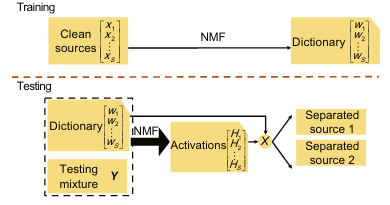
\includegraphics[scale=0.6]{obrazky-figures/nmf.png}
    \caption{\label{fig:nmf}Znázornění trénovací a testovací fáze. Obrázek byl inspirován \cite{speechseparation}}
\end{figure}

Stejně jako metoda CASA, i tato má mnoho nevýhod, které omezují její použití pro řešení reálných problémů separace.



\subsection{Hluboké neuronové sítě}
Nejlépe si při řešení problému koktejl párty vedou postupy založené na hlubokém učení a neuronových sítích.
Metody převáděly směs do časově--frekvenční reprezentace znázorněné na obrázku \ref{fig:spektrum} pomocí STFT (\textit{short time fourier transformation}).

\begin{figure}[H]
    \centering
    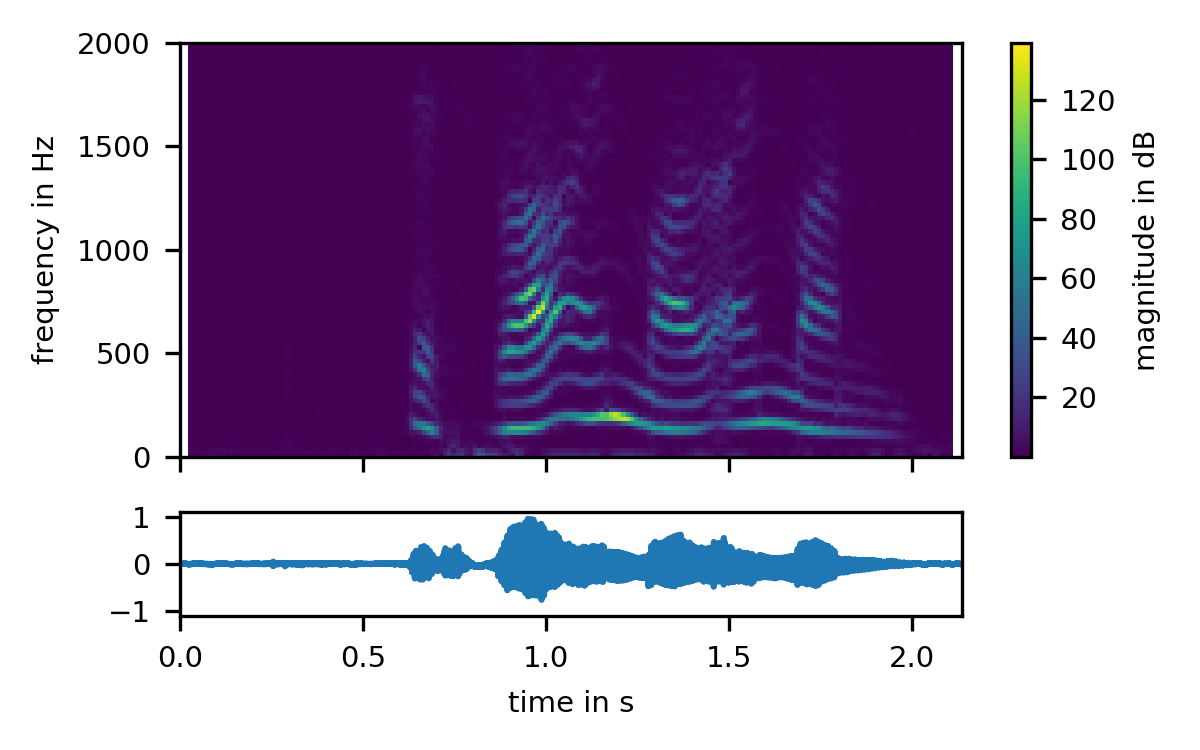
\includegraphics[scale=0.6]{obrazky-figures/spektrum.png}
    \caption{\label{fig:spektrum}Časově--frekvenční reprezentace řeči, neboli spektrum}
\end{figure}




\section{Vyhodnocovací metriky}
Pro vyhodnocení kvality separace se používají různé metriky. Jejich volba závisí na řešeném problému.


\subsection{Signal--to--noise ratio}
Nejzákladnější metrika pro určení kvality separace je signal--to--noise ratio (SNR), která porovnává zastoupení chtěného signálu a šumu v pozadí a je definována jako poměr energie originálního (ideálního) signálu a energie rozdílu mezi originálním a rekonstruovaným signálem.

\begin{equation}
  SNR = \frac{E_s}{E_N}
\end{equation}

Výsledný poměr často bývá vyjádřen v decibelech jako

\begin{equation}
  SNR(dB) = 10log_{10}\frac{E_s}{E_N}
\end{equation}

kde kladná SNR hodnota udává, že zastoupení signálu je větší, než zastoupení šumu \todo{citovat https://labrosa.ee.columbia.edu/~dpwe/pubs/Ellis04-sepeval.pdf}.



\subsection{SDR -- Source Distortion Ratio}
SDR je jedna z nejznámějších metrik pro měření kvality řečového signálu.


\subsection{PESQ -- Perceptual evaluation of speech qualit}
Procentuální vyhodnocení kvality řeči (PESQ\cite{pesq-itut}) je standardizovaná metrika pro vyhodnocování kvality řeči. Jeho hodnota se pohybuje od -0.5 do 4.5 s tím, že vyšší hodnota znamená lepší procentuální kvalitu\cite{DBLP:journals/corr/abs-1901-09146}.


\subsection{STOI}


Bylo navrženo mnoho konvenčních přístupů a metod pro řešení problému koktejl párty a s ním spojené separace mluvčích, ale většina z nich nedosahuje dostatečné přesnosti nebo výkonu k použití v reálných situacích. Přístupy založené na hlubokém učení a neuronových sítích předčily dosavadní techniky jak v přesnosti, tak ve výkonu, což umožňuje jejich nasazení v běžném životě.


%----------------------------------------------------------------------------------------------------------------------------------------------------------------------
\chapter{Neuronové sítě}
\label{neuronovky}
V~dnešní době zažívají neuronové sítě díky výkonosti počítačů velký rozmach. Jejich využití prostupuje skrze mnohé vědní obory a dokáží řešit celou řadu problémů, ve kterých dosahují výborných výsledků, které zdaleka předčily dosavadní postupy. 

Neuronové sítě (\textit{artificial neural networks}) jsou výpočetní model, který je inspirovaný strukturou lidského mozku, ve kterém je obrovské množství propojených a komunikujících neuronů. Ty se skládají ze vstupních dendridů, výstupních axonů a samotného těla neuronu. Na základě vnitřního potenciálu a vstupních hodnot je po přesažení prahové hodnoty neuron vybuzen a je vyslán signál na výstupní axon. Signál je nakonec předán dalším neuronům skrze jejich vstupní dendridy\cite[p.~65--66]{mitdeeplearning_small}.

Účelem neuronové sítě je naučit se plnit zadanou úlohu. Rozdíl oproti běžným algoritmům je ale ten, že způsob, jakým síť má problém řešit, není explicitně naprogramován, ale je postupně naučen. Základní způsoby učení jsou s~učitelem (\textit{supervised}) a bez učitele (\textit{unsupervised}). 

\textbf{Učení s~učitelem}, pod které spadá i tato práce, spočívá v~mapování vstupních dat na data výstupní na základě vzorových příkladů dvojic vstup--výstup. Množině takových dvojic se říká trénovací dataset. Další vlastností trénovacích dat určených pro učení s učitelem, je jejich označení (\textit{label}).

Mezi problémy, které se dají řešit neuronovými sítěmi patří klasifikační a regresní problémy. Konkrétní příklad z~oblasti klasifikace může být rozpoznávání objektů na obraze, psaného písma nebo detekce obličejů na videu, ale i mnohé aplikace ve zpracování řeči. Některé z problémů lze řešit sítí, která se skládá z jednotek neuronů, zatímco složitější problémy vyžadují mnohem větší kapacitu sítě a ta pak může obsahovat i tisíce neuronů.

Upravovat samotnou strukturu a chování neuronové sítě lze pomocí jejích hyperparametrů, což jsou parametry určující nastavení neuronové sítě a trénovacího algoritmu. Tyto parametry musí být určeny před začátkem trénování a většinu nelze později měnit. Mohou určovat kapacitu modelu, velikost záběrného pole, velikost filtrů, ale i regulovat samotný proces učení nastavením počtu epoch, po které se model má učit, nebo také počet dat předaný v jedné dávce (tzv. \textit{minibatches}) během učení sítě.


\section{Organizace feedforward sítí}
Feed forward neuronové sítě (\textit{Multi Layer Perceptron -- MLP}) jsou typ umělých neuronových sítí, kde se nevyskytují cykly ve výpočetním grafu, tedy zpětná propojení vrstev, takže informace se pohybuje pouze jedním směrem, od vstupní vrstvy přes skryté vrstvy až po vrstvu výstupní. Sítě, které obsahují cykly, se nazývají rekurentní. Rozdíl znázorňuje obrázek \ref{fig:netcomparison}.

\begin{figure}[H]
    \centering
    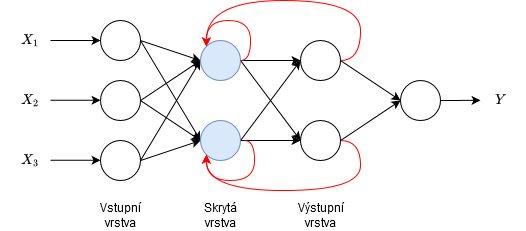
\includegraphics[scale=0.5]{obrazky-figures/feedforward_vs_recurrent.png}
    \caption{\label{fig:netcomparison}Příklad grafu feed forward sítě a rekurentní neuronové sítě. Lze si všimnout orientace šipek u~feed forward sítě, které směřují pouze jedním směrem, zatímco u~rekurentní sítě šipky směřují i k~předešlým uzlům grafu\cite{FFandRecNN}.}
\end{figure}

Struktura neuronové sítě je organizována do vrstev, které se skládají z~neuronů. Feedforward síť je tvořena třemi typy vrstev (viz obrázky \ref{fig:netcomparison} a \ref{fig:mlp}). Vstupní vrstva slouží k~předání hodnot do sítě, ale nijak tyto hodnoty nemodifikuje. Nezměněné jsou zkopírovány do první skryté vrstvy. Následují skryté vrstvy, z~nichž poslední je napojena na výstupní vrstvu. Ta má obvykle méně neuronů než předešlé vrstvy a hodnoty na výstupu mohou představovat třídy, do kterých má být klasifikován vstup v případě klasifikátorů, nebo predikce hodnot na základě vstupních dat v případě regrese. S~počtem jednotlivých vrstev souvisí pojem hloubka sítě, která je rovna počtu všech vrstev neuronové sítě od vstupní až po výstupní vrstvu. Pojem \todo{uvozovky lepe} "hluboká neuronová síť" označuje takovou síť, která má dvě nebo více skrytých vrstev. Existuje mnoho typů vrstev, například plně propojené, pooling, s~přeskočením nebo vrstvy konvoluční.

\begin{figure}[H]
    \centering
    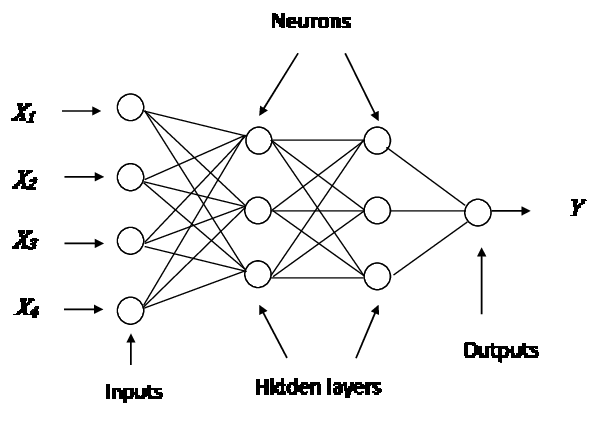
\includegraphics[scale=1.3]{obrazky-figures/mlp.png}
    \caption{\label{fig:mlp}Schéma neuronové sítě, která má 2 skryté vrstvy}
\end{figure}


\section{Umělý neuron}
Základní stavební jednotka neuronových sítí je umělý neuron (\textit{artificial neuron}) (viz obrázek \ref{fig:neuron}). Tento model je založen na principu reálných neuronů, které se nacházejí v~organizmech. Umělý neuron obsahuje libovolně mnoho vstupních propojení, přes které se mu předávají data v~podobě vstupního vektoru $\overrightarrow{x} = [x_1, x_2, \dots, x_n], x_n \in \mathbb{R}$. Sám neuron obsahuje hodnotu bias $b \in \mathbb{R}$ a vektor vah $\overrightarrow{w} = [w_1, w_2, \dots, w_n], w_n \in \mathbb{R}$, jenž je upravován během trénování neuronu.

Výstupní hodnota závisí na vstupních datech, aktuálním vnitřním stavu (hodnoty vah a biase) a na zvolené aktivační funkci. Vstupní hodnoty jsou váhovány, což znamená, že každá vstupní hodnota je vynásobena s~váhou na daném vstupním spojení. S~použitím definovaných vektorů lze napsat, že vstupní vektor je vynásoben s~vektorem vah.

\begin{figure}[H]
    \centering
    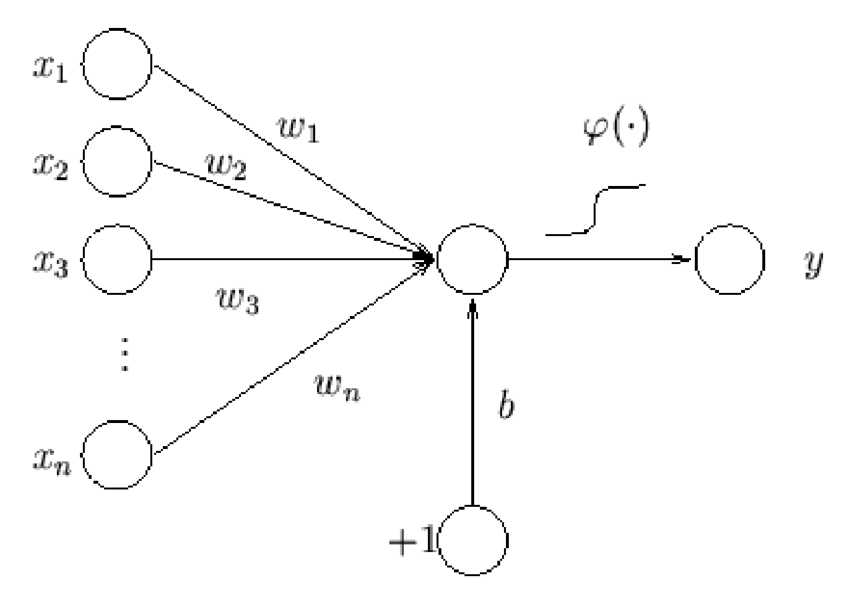
\includegraphics[scale=0.35]{obrazky-figures/perceptron.png}
    \caption{\label{fig:neuron}Schéma umělého neuronu}
\end{figure}

Hodnota bias $b$, která je přičtena k~sumě násobků vah a vstupních hodnot, je prahová hodnota modifikující dobu, kdy se aktivuje neuron a změní svůj výstup. Matematicky to znamená, že s~grafem aktivační funkce horizontálně pohybuje doleva nebo doprava v~závislosti na tom, je-li hodnota biasu pozitivní nebo negativní. Toto posunutí je znázorněno na obrázku \ref{fig:bias}. V~závislosti na řešeném problému může být žádoucí, aby i hodnota bias byla modifikována během učení společně s~ostatními váhami. V~opačném případě je hodnota nastavena pevně na nějakou konstantní hodnotu, obvykle na hodnotu jedna.

\begin{figure}[H]
    \centering
    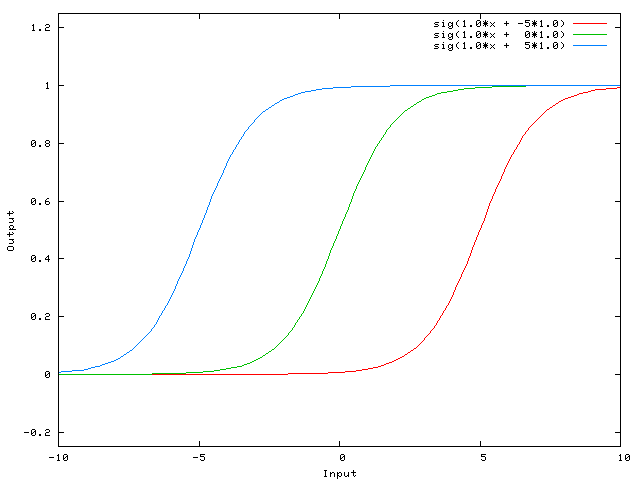
\includegraphics[scale=0.4]{obrazky-figures/bias.png}
    \caption{\label{fig:bias}Vliv hodnoty bias na aktivační funkci}
\end{figure}




Výstup neuronu se vypočítá jako
\begin{equation}
	y = f\Big((\sum_{k=1}^n w_kx_k) + b\Big)
\end{equation}
kde $f$ je aktivační funkce, $x_k \in \mathbb{R}$ je vstupní hodnota, $w_k \in \mathbb{R}$ je váha, kterou se vstupní hodnota vynásobí a $b \in \mathbb{R}$ je hodnota bias.


\section{Aktivační funkce}
Aktivační, neboli prahová funkce, určuje výstupní hodnotu neuronu. Funkce se vybírá na základě problému, který se má neuronová síť naučit řešit. Správná volba aktivační funkce vede k~lepší konvergenci učení sítě. Naopak špatná volba může vést ke stále větší odchylce od správného řešení -- může divergovat. Povaha problému může vyžadovat specifické vlastnosti aktivační funkce - lineární nebo nelineární. Pro nestandardní problémy je obvykle potřeba experimentálně zjistit, která funkce bude nejlépe vyhovovat danému problému. 

Pokud by veškeré aktivační funkce v~modelu byly lineární, tak celkové mapování sítě by bylo omezeno pouze na lineární mapování vstupu na výstup. Reálné problémy ale lineární obvykle nejsou a v~případě pokusu modelovat takovým modelem nelineární vztahy by vedlo k~velice nepřesným výsledkům, který by byl zapříčiněn podučením (\textit{underfitting}), což znamená, že model, který se učí zakódovat nějaký vzor v~datasetu, je příliš jednoduchý. Proto je potřeba zavést do modelu i nelineární aktivační funkce, které tento problém řeší\cite[p.~77--78]{mitdeeplearning_small}.

Z~pohledu učení je také důležité, aby aktivační funkce byla diferencovatelná. To umožňuje použití učících metod založených na výpočtu gradientu, jako je algoritmus backpropagation.



\subsection*{Sigmoid}
\begin{equation}
  f(x) = \frac{1}{1+\exp(-z)}
\end{equation}

\todo{popsat}

\begin{figure}[H]
    \centering
    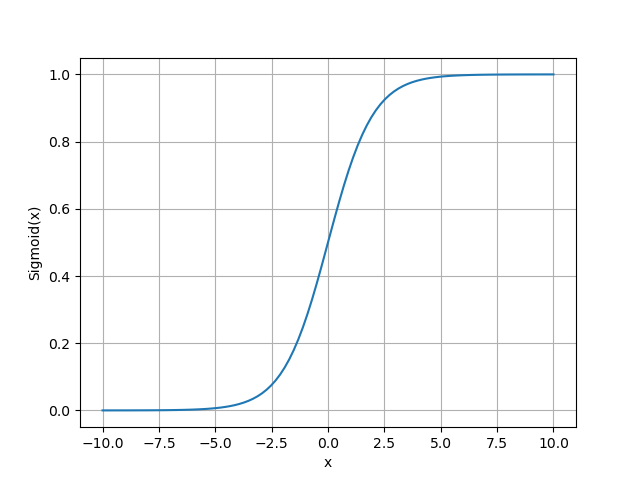
\includegraphics[scale=0.18]{obrazky-figures/sigmoid.png}
    \caption{\label{fig:sigmoid}Graf aktivační funkce sigmoid}
\end{figure}



\subsection*{Softmax}
\begin{equation}
  f(x) = \frac{1}{1+\exp(-z)}
\end{equation}

\todo{popsat}

\begin{figure}[H]
    \centering
    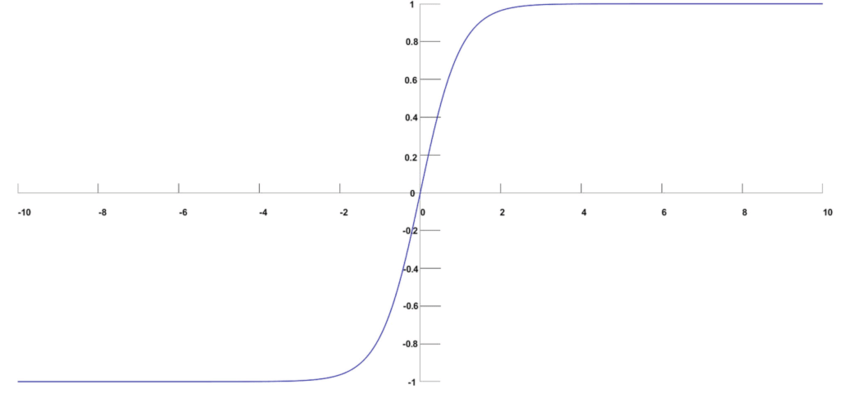
\includegraphics[scale=0.35]{obrazky-figures/softmax.png}
    \caption{\label{fig:softmax}Graf aktivační funkce softmax}
\end{figure}




\subsection*{ReLU}
Rectified Linear Unit je nejčastěji používaná aktivační funkce. Vyžaduje-li neuronová síť nějakou nelinearitu, je ReLU pro většinu případů ideální. Pro každou zápornou hodnotu $x$ vrací $0$ a pro kladnou hodnotu $x$ vrací tutéž hodnotu $x$, jak udává rovnice 
\begin{equation}
   f(x)=max(0,x)
\end{equation}

\begin{figure}[H]
    \centering
    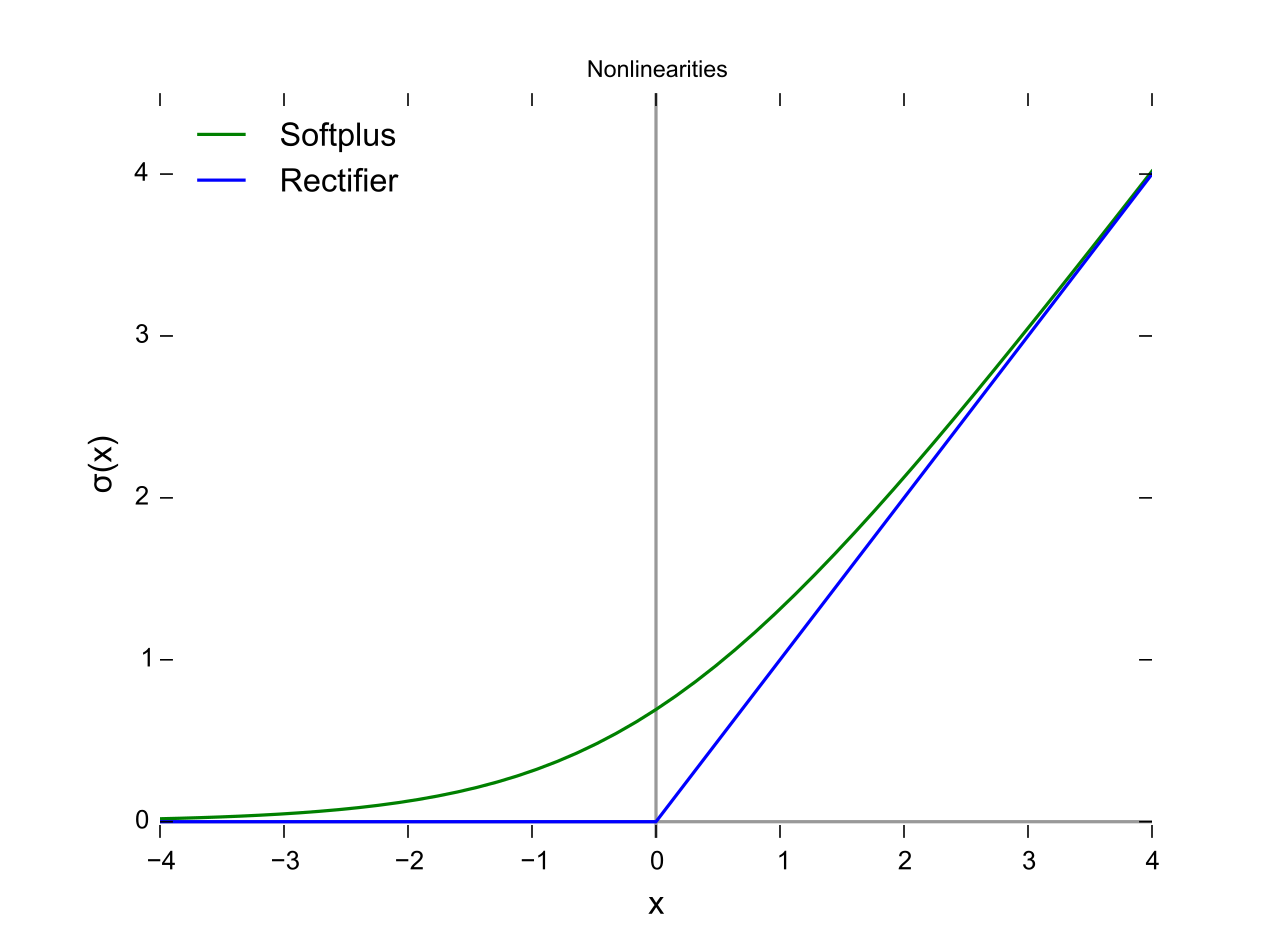
\includegraphics[scale=0.2]{obrazky-figures/ReLU.png}
    \caption{\label{fig:relu}Graf aktivační funkce ReLU}
\end{figure}




\subsection*{PReLU}
Parametrizovaná ReLU je nelineární aktivační funkce, která se používá v~případě, že chceme produkovat na výstup malý nenulový gradient i v~případě záporné vstupní hodnoty $x$. V~tom případě je vstupní hodnota vynásobena parametrem $\alpha$ a to představuje výsledek. Parametr $\alpha$ se společně s~ostatními váhami učí během učícího procesu.
\begin{equation}
  f(x) =
  \begin{cases}
    x & \text{if } x \geq 0 \\
    {\alpha}x & \text{if } x < 0
  \end{cases}
\end{equation}

\begin{figure}[H]
    \centering
    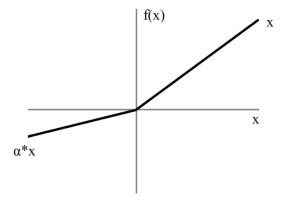
\includegraphics[scale=1.4]{obrazky-figures/prelu.jpg}
    \caption{\label{fig:prelu}Graf aktivační funkce PReLU}
\end{figure}


\section{Lineárně separovatelná data}
Síť složená z~jediného neuronu by byla omezena pouze na klasifikaci lineárně separovatelných dat. To jsou taková data, která lze rozdělit, existuje-li alespoň jedna přímka v~rovině taková, že na jedné straně přímky jsou všechna data klasifikována do první třídy, a na druhé straně data klasifikována do třídy druhé, jak lze vidět na obrázku \ref{fig:linear_separable}.

\begin{figure}[H]
    \centering
    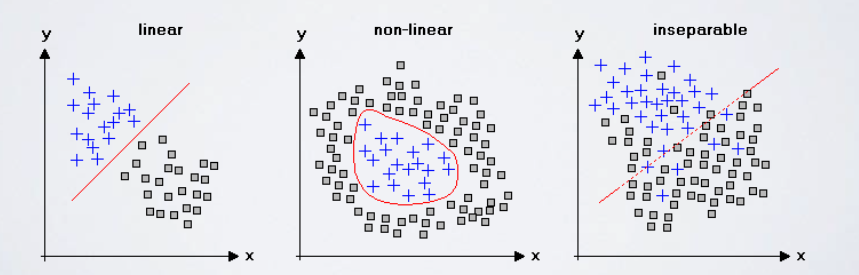
\includegraphics[scale=0.38]{obrazky-figures/linear_separable.png}
    \caption{\label{fig:linear_separable}Lineárně separovatelná (vlevo) a neseparovatelná (vpravo) data} 
\end{figure}

Mějme množinu dat, kterou tvoří dvě rozdílné třídy objektů $\Omega_1, \Omega_2 \subset \mathbb{R}^m$. Třídy jsou lineárně separovatelné, jestliže existuje $w \in 
\mathbb{R}^m$ a $\theta \in \mathbb{R}$ takové, že 
\begin{equation}
   \forall x \in \Omega_1 : x^Tw > \theta
\end{equation}
\begin{equation}
   \forall x \in \Omega_2 : x^Tw < \theta
\end{equation}

Problém lze zobecnit tak, že řešením bude separace tříd pomocí hyper roviny v~prostoru $\mathbb{R}^m$, jak zachycuje obrázek \ref{fig:hyperplane_separable}
\cite{linearseparability}.

\begin{figure}[H]
    \centering
    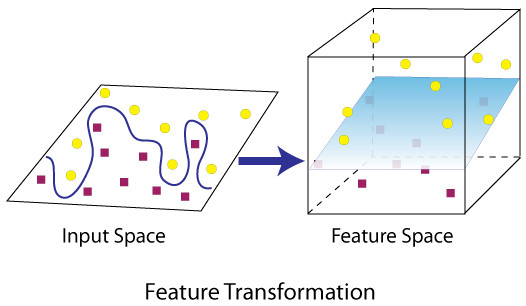
\includegraphics[scale=0.8]{obrazky-figures/hyperplane_separable.jpeg}
    \caption{\label{fig:hyperplane_separable}Separace pomocí hyper roviny} 
\end{figure}

Neuron se nedokáže ale naučit klasifikovat třeba funkci XOR, protože ta není lineárně separovatelná. Byly by zapotřebí minimálně dvě přímky pro rozdělení dat, jak zobrazuje obrázek \ref{fig:xor}\todo{citovat xor}. K~překonání tohoto problému se neurony spojují do podoby neuronové sítě, která dokáže řešit libovolně komplexní problémy.

\begin{figure}[H]
    \centering
    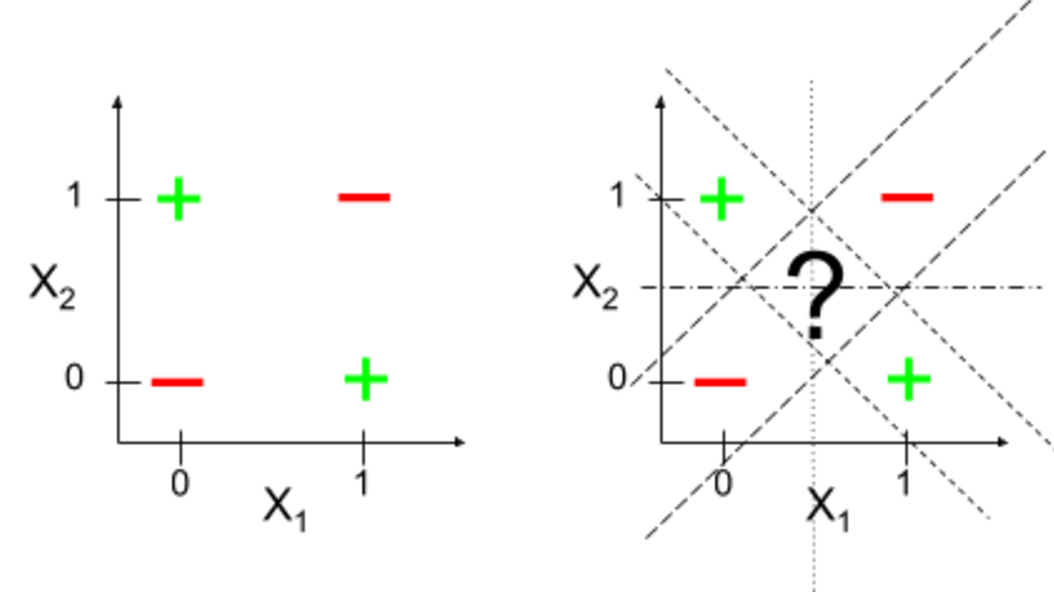
\includegraphics[scale=0.3]{obrazky-figures/xor.png}
    \caption{\label{fig:xor}Graf funkce XOR, jejíž výstup není lineárně separovatelný} 
\end{figure}





\section{Konvoluční neuronové sítě}
\todo{Nebo to pojmenovat jako Konvolucni vrstva?}.
Konvoluční neuronové sítě jsou typ feedforward sítí, které neobsahují pouze plně propojené vrstvy, ale také vrstvy konvoluční.
\begin{figure}[H]
    \centering
    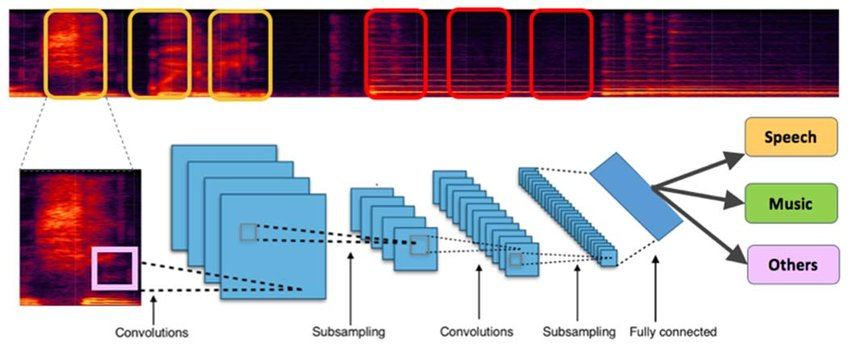
\includegraphics[scale=0.5]{obrazky-figures/conv_nn_audio.jpg}
    \caption{\label{fig:conv_nn}Konvoluční neuronové sítě}
\end{figure}

\subsection{Konvoluční vrstva}
Diskrétní konvoluce je definována jako

%\begin{equation}
%   (f * g)_k = \sum_{i=-\inf}^{\inf} f_i g_{k-i} = \sum_{i=-\inf}^{\inf} f_{k-i} g_{i}
%\end{equation}

kde $\star$ je konvoluční operátor, $f$ je funkce signálu, funkce $g$ je konvoluční jádro a $f_i$ a $g_i$ jsou hodnoty funkce na indexu $i$.



\section{Učení neuronových sítí}
Cílem trénování je naučit neuronovou síť vykonávat nějaký úkol. Trénování založené na metodě učení s učitelem vyžaduje dostatečně velký dataset obsahující dvojice vstup--výstup a obnáší volbu objektivní funkce, kterou se během trénování snažíme minimalizovat. 

Formálně je cílem učení aproximovat nějakou funkci $f^\ast$. Síti je předána vstupní hodnota $x$, pro kterou síť definuje mapování na výstupní hodnotu jako $y = f(x; \theta)$, kde $\theta$ je parametr, který se síť učí tak, aby dosáhla nejlepší aproximace funkce. \cite[p.~163]{mitdeeplearning}.


\subsection{Objektivní funkce}
Objektivní funkce (loss funkce, cost funkce) je funkce, která je během učení minimalizována nebo maximalizována, v závislosti na konkrétním úkolu a kontextu použití. Tato funkce mapuje událost či hodnoty na reálné číslo reprezentující \todo{spravit uvozovky} "cenu", která je asociována s touto událostí či hodnotami. Je--li tato funkce použita pro optimalizační problém, pak je cílem hodnotu minimalizovat a funkci se pak říká loss funkce, protože její výstupní hodnota nám udává velikost chyby, která se počítá na základě rozdílu mezi výstupem sítě a odpovídajícími trénovacími daty z datasetu. Pak platí, že čím menší chyba, tím lépe síť provádí svůj úkol, na který je trénována. Použije--li se hodnota objektivní funkce s opačným znaménkem, tak lze funkci použít jako hodnotící metriku.

V rámci učení sítě je žádoucí, aby gradient objektivní funkce byl dostatečně velký (prudký) a předvídatelný. V takovém případě bude dobře sloužit pro účely trénování. V případě malého gradientu by funkce saturovala (byla by příliš plochá) a to by mohlo negativně ovlivnit trénování sítě \cite{mitdeeplearning}. 

Nejčastěji se pro regresní problémy používají objektivní funkce \textit{Mean Squared Error Loss} a \textit{Mean Absolute Error Loss}.


\subsection*{MSELoss (Mean Squared Error Loss)}
MSELoss je nejčastěji používaná objektivní funkce při řešení regresních problémů. Vypočítá se jako
\begin{equation}
  MSE = \frac{1}{N}\sum_{i=1}^N(y_i - \hat{y_i})^2
\end{equation}
kde $N$ je počet trénovacích dat v datasetu, $y_i$ je předpovězená hodnota a $\hat{y_i}$ je odhadnutá hodnota. Vzhledem k druhé mocnině je výsledek vždy pozitivní nezávisle na znaménku hodnot $y_i$ a $\hat{y_i}$, jak lze vidět na obrázku \ref{fig:mseloss}. Druhá mocnina také zajišťuje, že čím větší je rozdíl mezi předpovídanou a aktuální odhadnutou hodnotou, tím více se chyba projeví. Funkce dosahuje L2 regularizace.

\begin{figure}[H]
    \centering
    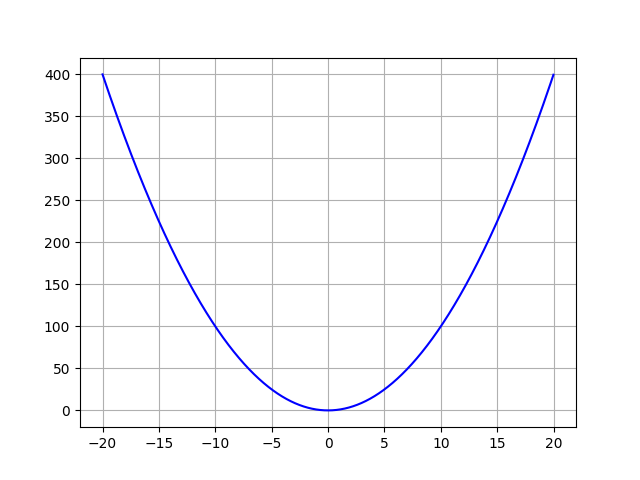
\includegraphics[scale=0.4]{obrazky-figures/mseloss.png}
    \caption{\label{fig:mseloss}Graf objektivní funkce MSE Loss}
\end{figure}


\subsection*{MAELoss (Mean Absolute Error Loss)}
\todo{graf a popsat a rozdily a vyhody}
MAE je velmi podobná objektivní funkce jako MSE, ale s téměř opačnými vlastnosti. Stejně jako MSE, ani tato funkce nenabývá negativní hodnoty, ale narozdíl od MSE, která má tuto vlastnost díky druhé mocnině rozdílu, MAE toho dosahuje tak, že rozdíl předpovídané hodnoty $y_j$ a odhadnuté hodnoty $\hat{y_j}$ je uzavřen v absolutní hodnotě. Vypočítá se jako

\begin{equation}
  MAE = \frac{1}{N}\sum_{j=1}^N|y_j - \hat{y_j}|
\end{equation}

Výhodnou MAE je její lineární průběh, takže se větší chyby projeví úměrně více než chyby menší, oproti MSE, kde je závislost kvadratická. Nevýhodou je, že kvůli absolutní povaze není diferencovatelná v hodnotě $x=0$, což může mít negativní následky pro výpočet gradientu.

\begin{figure}[H]
    \centering
    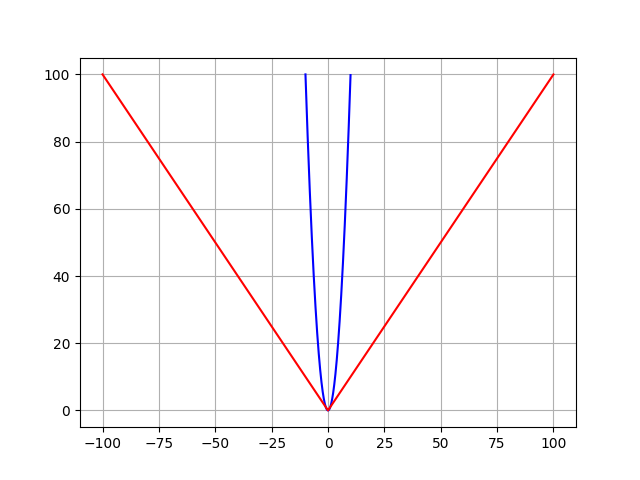
\includegraphics[scale=0.4]{obrazky-figures/maeloss.png}
    \caption{\label{fig:maeloss}Graf objektivní funkce MAE Loss (červeně)}
\end{figure}

\todo{Hinge loss?}


\subsection{Backpropagation}
Backpropagation (backprop) je algoritmus typu učení s učitelem pro učení neuronových sítí. Algoritmus zpětně prochází neuronovou síťí a na základě hodnoty cost funkce $J(\theta)$ počítá její gradient metodou \textit{gradient descent}. Cílem je upravit všechny váhy v síti na základě toho, jak moc každá váha přispívá k celkové chybě. Algoritmus backpropagation počítá řetězové pravidlo (\textit{chain rule}).

Algoritmus se skládá ze 3 opakujících se kroků. Prvním krokem je forward fáze, ve které se počítá pro každou dvojici vstupu a referenčního výstupu 


\cite{web-brilliant}
\cite[p~197]{deeplearning}


- zpetne sireni chyby
- adaptacni algoritmus, podil neuronu na chybe,
- 3 opakujici se faze uceni:

1) feedforward - dopredu
2) zpetne sireni chyby - Backpropagation
3) uprava vah a biasu na zaklade chyby pomoci gradient descent
- chain rule



\subsection*{Gradient descent}
Gradient descent je iterativní optimalizační algoritmus pro hledání lokálního minima diferencovatelné objektivní funkce $J(\theta)$, kde $\theta \in \mathbb{R}^d$ reprezentuje učené parametry modelu, úpravou těchto parametrů v opačném směru, než je hodnota gradientu. Výpočet je prováděn postupným pohybem ve směru největšího klesání, které je určeno zápornou hodnotou gradientu. Rychlost pohybu závisí na velikosti kroku, což udává \textit{learning rate}. Správná volba \textit{learning rate} ovlivňuje rychlost, jakou je nalezeno minimum funkce. Při nízké hodnotě bude výsledek přesnější, ale nalezení minima bude výpočetně náročnější, protože v každém kroku se počítá nová hodnota gradientu. Při větší hodnotě je riziko, že minimum bude přeskočeno\cite{ruder2016overview}.
\begin{figure}[H]
    \centering
    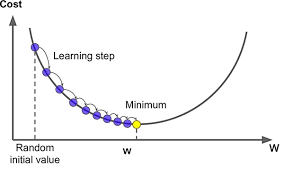
\includegraphics[scale=0.7]{obrazky-figures/gradientdescent.png}
    \caption{\label{fig:gradientdescent}Ukázka algoritmu gradient descent při hledání minima dané funkce postupným přibližováním dle nastavené velikosti kroku}
\end{figure}


\todo{popsat vice vliv LR na loss}


\subsection{Underfitting a generalizace}
Generalizace, neboli \textit{test error}, je vlastnost modelu, která udává, jak dobře model pracuje s dříve neviděnými daty, tedy s daty, které nebyly použity pro jeho učení. Během učení vzniká učící chyba, která je trénováním postupně minimalizována, ale kvalita modelu je pak měřena na testovacích datech. 
Testovací chyba by ideálně měla být co nejblíže chybě na trénovací sadě. Z rozdílu mezi těmito chybovými hodnotami se dají diagnostikovat problémy s naučením sítě -- podučení (\textit{underfitting}) a přeučení(\textit{overfitting}). 

\textit{Underfitting} nastane v případě, že model se již nedokáže v důsledku jeho kapacity zmenšit dostatečně jeho chybovou hodnotu na trénovacím datasetu.

\textit{Overfitting} nastane, když rozdíl mezi trénovací chybou a testovací chybou je příliš velký.

Kapacita je vlastnost modelu určující, kolik se toho dokáže model naučit. V případě nízké kapacity se model nedokáže naučit všechny příznaky z trénovacích dat a v případě vysoké kapacity se mohou přeučit zapamatováním si jejich příznaků a tím sice dosáhnou nízké trénovací chyby, ale špatných výsledků během testování\cite[p107]{mitdeeplearning}.
\begin{figure}[H]
    \centering
    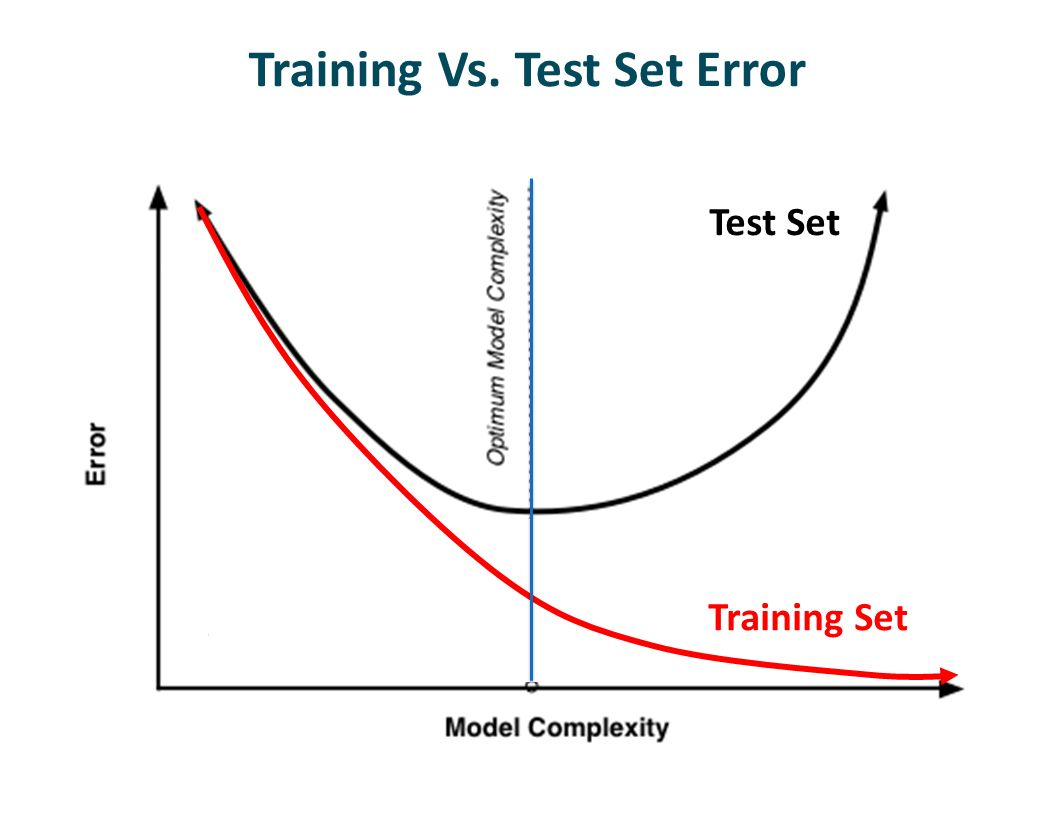
\includegraphics[scale=0.3]{obrazky-figures/capacity_vs_error.jpg}
    \caption{\label{fig:gradientdescent}Vliv kapacity modelu trénovací a testovací chybu. Obrázek inspirován podle \cite{trainingvstesterror}}
\end{figure}


\subsection{Regularizace}
Regularizace je souhrn postupů, které říkají, jak modifikovat učící algoritmus tak, aby se zredukovala chyba generalizace, zatímco testovací chyba zůstane stejná\cite[p117]{mitdeeplearning}.


\subsection{Residuální spojení}
\todo{Toto chce obrazek residualniho spojeni. Popsat. Citovat odnekud, proc jsou residualni spojeni dobra pro trenovani DeepNN a v jednom odstavci to nejak shrnout}.


\subsection{Význam validační množiny v~trénování}
\todo{Mozna ne jako subsekci ale jen jako jeden odstavec}
Většina algoritmů strojového učení má nějakou sadu hyperparametrů, kterou je upravováno chování algoritmu. Hodnoty hyperparametrů obvykle bývají nastavovány ručně ještě před spuštěním procesu učení a hodnota se v~průběhu nemění, protože hodnoty by bylo obtížné optimalizovat. 
Některá nastavení se nicméně mohou stát hyperparametrem a být upravována během trénování, ale není vhodné je měnit na základě výsledku učení na trénovací sadě, protože by mohlo dojít k~přetrénováníoverfitting) v~důsledku \todo{CEHO??}. Pro tento případ potřebujeme validační sadu, která je odlišná od trénovací sady.
Po každém zpracování trénovací sady následuje validační sada, po jejímž skončení jsou optimalizovány hyperparametry[][].
\todo{[kniha 117-118] kap 5.3 = Hyperparameters and validation set} 
\todo{najit jeste nejakej zdroj s~popisem a pripadne nejaky zajimavejsi info.}


V této kapitole byly popsány základní principy neuronových sítí, jejich základní struktura a stavební bloky. V návaznosti na to byly zmíněny konvoluční sítě, které jsou pro tuto práci stěžejní. Dále byl popsán proces trénování sítí a algoritmy back--propagation a gradient descent. Nakonec byly zmíněny některé oblasti, které se zabývají optimalizacemi sítě, kladoucí si za cíl zlepšit například dobu trénování nebo kvalitu naučení sítě, což může mít za následek lepší výkon sítě při její evaluaci nebo umožnit nasazení ve zdrojově omezeném prostředí.

%----------------------------------------------------------------------------------------------------------------------------------------------------------------------
%----------------------------------------------------------------------------------------------------------------------------------------------------------------------
\chapter{TasNet - Time--Domain Audio Separation Network}
\label{tasnet}

Tato kapitola vychází z referenční studie \textbf{TasNet: Surpassing Ideal Time-Frequency Masking for Speech Separation}\cite{luo2018convtasnet} a popisuje její navrhnuté řešení pro separaci mluvčích v časové doméně.

Přestože metody pro zpracování řeči v akustickém přostředí, ve kterém se může současně prolínat mnoho řečových signálů, v poslední době zaznamenaly velké zlepšení, stále trpí mnoha nedostatky. Přesnost systémů, odezva a nároky na výpočetní výkon jsou u těchto metod natolik zásadní, že znemožňují nebo velmi omezují jejich nasazení mimo výzkumné prostředí, například v aplikacích, které by mohly zpracovávat řeč v reálném čase.

Většina dosavadních postupů byla založena na převodu směsi řečových signálů do časově--frekvenční (T--F) reprezentace (spektrogramu) pomocí STFT (Short--Time Fourier Transformation)\cite{10.1109/TASLP.2018.2842159}. Tento převod ale měl pro využití v reálném čase příliš vysokou odezvu a navíc T--F reprezentace nebyla optimalizovaná pro separaci mluvčích.

Pro překonání nedostatků předešlých metod byla navržena architektura Time--domain Audio Separation Network (TasNet), založena na hlubokém učení a neuronových sítích, která používá konvoluční enkodér k převodu směsi na reprezentaci, která je optimalizovaná pro extrakci jednotlivých mluvčích. Samotné separace je docíleno aplikací masek na reprezentaci. Masky jsou odhadnuty v TCN, která je tvořena opakující se posloupností konvolučních bloků se zvyšující se časovou dylatací. Po aplikaci masek jsou separovaní mluvčí rekonstruováni konvolučním dekodérem.

\todo{uvod do kapitoly - co je tasnet, nastin jak funguje - kroky, masky, encoder, TCN, }


\begin{figure}[H]
    \centering
    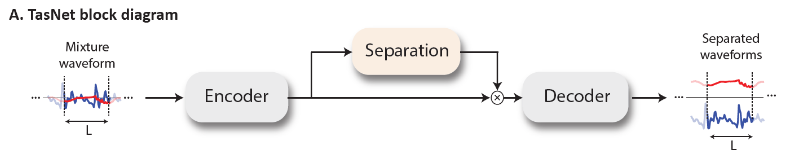
\includegraphics[scale=0.5]{obrazky-figures/tasnet-pipe.png}
    \caption{\label{fig:tasnet-pipe}Zjednodušený model architektury}
\end{figure}


\section{Konvoluční auto--enkodér}
\todo{Konvoluční autoenkodér, vstup, výstup...}

- schema bez separacniho modulu
- non negative representation of audio
\begin{figure}[H]
    \centering
    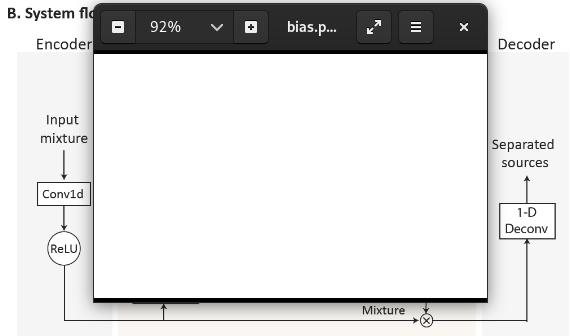
\includegraphics[scale=0.5]{obrazky-figures/tasnet-autoencoder.png}
    \caption{\label{fig:tasnet-autoencoder}Schéma konvolučního autoenkodéru}
\end{figure}

\subsection{Enkódování směsi}


\subsection{Dekódování}


\section{Separační modul}
- odhad masek pro jednotlive mluvci
- schema se separacnim modulem
\begin{figure}[H]
    \centering
    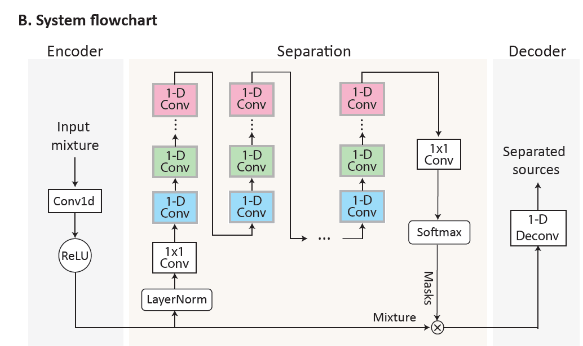
\includegraphics[scale=0.6]{obrazky-figures/tasnet-architecture.png}
    \caption{\label{fig:tasnet-modul}Schéma architektury TasNet}
\end{figure}


\subsection{Temporal Convolutional Network}
\todo{TCN, dilatace, stacked blocks, X, R}


\subsection{Konvoluční bloky}
- Z~čeho se skládá -- konvoluční vrstvy, normalizace
- diagram konv bloku.
- Mozna: Dilatace a increasing time perception
\begin{figure}[H]
    \centering
    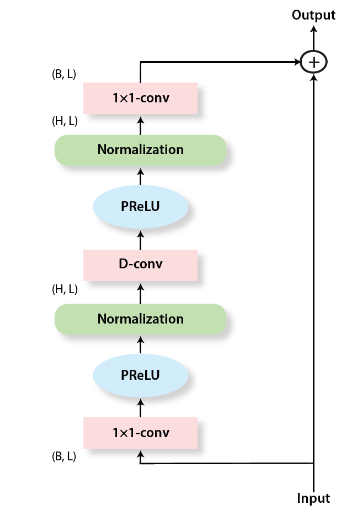
\includegraphics[scale=0.5]{obrazky-figures/conv-res-block.png}
    \caption{\label{fig:tasnet-convblock}Jeden konvoluční blok}
\end{figure}


\todo{zaver kapitoly}

%----------------------------------------------------------------------------------------------------------------------------------------------------------------------


\chapter{Implementace sítě}
\label{implementace}
Pro implementaci neuronových sítí vzniklo mnoho frameworků jako pytorch, tensorflow, keras a další, které umožňují síť poskládat z již předdefinovaných modulů. Jejich vlastnosti lze modifikovat dle potřeby pomocí argumentů při jejich instanciaci nebo při jejich použití. Kromě těchto bloků a mnoha dalších možností frameworky obsahují i metody pro práci s datasety, funkce pro vykreslování grafů a pro matematické operace.

Mým úkolem bylo implementovat neuronovou síť podle architektury TasNet pro separaci mluvčích v časové doméně. V rámci zadání jsem si zvolil použít framework s názvem pytorch\footnote{\url{https://pytorch.org/}}, který má kvalitní dokumentaci a aktivní uživatelskou základnu. Pytorch funguje nad jazykem Python\footnote{\url{https://www.python.org/}} a v celé práci používám jeho aktuálně nejnovější verzi (Python 3.8.2) a mimo jiné podporuje práci s datasety, včetně implementace vlastního nahrávání a manipulace s daty. Základní jednotkou, se kterou síť pracuje, je tensor. Ve frameworku pytorch je \textbf{torch.Tensor} třída reprezentující multidimenzionální matici obsahující data jednoho typu. Na tensory jsou převáděna data během načítání datasetu a následně předávána síti ke zpracování. Samotná implementace probíhala na systému Kali linux (4.19.0-kali5-amd64), který je založený na systému Debian. Aplikace byla vyvíjena v textovém editoru Vim\footnote{\url{https://www.vim.org/}} a byla během implementace spouštěna a testována v příkazovém procesoru Bash\footnote{\url{https://www.gnu.org/software/bash/}} (Bourne Again SHell) verze 5.0.16. Bash jsem zvolil i pro implementaci některých pomocných skriptů kvůli jednoduchému spouštění z terminálu a možnostem automatizace některých opakujících se příkazů. Pro správu verzí jsem používal verzovací systém Git\footnote{\url{https://git-scm.com/}}.

Trénování sítě probíhalo z~počátku na CPU \textit{intel i5} mého osobního notebooku \textit{Lenovo Y50-70}, což se ale ukázalo jako naprosto nevhodné vzhledem k náročnosti výpočtu kvůli nedostatečnému výkonu. Začal jsem tedy používat službu \textit{Google colab}, která poskytuje na omezenou dobu (12 hodin) stroje, které navíc obsahují technologii \textit{cuda}, což mi umožňilo výpočet provádět na GPU, čímž se trénování zrychlilo několikanásobně. Ještě více pomohlo předplacení služby, čímž se mi prodloužila doba, po kterou jsem mohl síť trénovat, na 24 hodin a zvýšila se šance na získání silnějších strojů. Modely byly trénovány na GPU \textit{T80} a \textit{T100} v závislosti na tom, která z nich mi zrovna byla přidělena pro dané sezení (\textit{session}). 

\bigskip
\todo{zamyslet se co tu chci ukazat v tom algu, pripadne vypustit parsovani, instanciaci atd}
\begin{algorithm}[H]
 \LinesNumbered
 parsování argumentů programu\;
 instanciace modelu TasNet\;
 \If{$args.checkpoint != NULL$}{
	načtení checkpointu\; 
 }
 instanciace třídy SegmentDataset a dataloaderu pro trénovací data\;
 instanciace třídy SegmentDataset a dataloaderu pro validační data\;
 \For{epocha v args.Epochs}{
  \tcc{trénování}
  loss = 0\;
  \For{směs\_mluvčích z trénovacího datasetu}{
    \tcc{cyklus načítá z dataloaderu segmenty nahrávek, které jsou generovány v třídě SegmentDataset}
  	$odhadovaná\_separace = TasNet(směs\_mluvčích)$\;
  	$loss = sisnr(optimální\_separace, odhadovaná\_separace)$\;
  	propagace chyby a úprava vah\;
  }
  \tcc{validace}
  vypnout gradient\;
  \For{směs\_mluvčích z validačního datasetu}{
  	$odhadovaná\_separace = TasNet(směs\_mluvčích)$\;
  	$validacni\_loss = sisnr(optimální\_separace, odhadovaná\_separace)$\;
  	\If{hodnota validační loss neklesla potřetí v řadě}{
		$learning\_rate = learning\_rate / 2$\;
  	}
  }
  na konci epochy uložit checkpoint\;
 }
 \caption{\label{alg:zakladnibeh}Zjednodušený algoritmus běhu programu pro trénování sítě}
\end{algorithm}

%------------------

\section{Implementace modelu}
\todo{today DNES - miniuvod k implementaci modelu - nic podrobneho, je to uz zmineno predtim ze to je v pytorchi atd}
\todo{Pozn: pytorch, scripty, tridy, moduly, parametry a volby spusteni}


Model se skládá ze separační části, která se skládá z konvolučních bloků, dále z...



\subsection*{Třídy SegmentDataset a AudioDataset}
\todo{zpracovani datasetu, jedna segmentuje, druha ne}
Blizsi popis segmentace v podkapitole \ref{sec:segmentace}.

%------------------

\subsection*{Třída Tasnet}
Třída Tasnet.py reprezentuje model neuronové sítě. Atributy třídy představují jednotlivé vrstvy neuronové sítě. Síť obsahuje konvoluční vrstvy, enkodér, dekodér a \textit{temporal convolutionan network}, která je tvořena sekvencí konvolučních bloků, které jsou zmíněny dále. V této třídě jsou také inicializovány váhy algoritmem xavier\todo{citovat}. Ve funkci $forward()$, která je volána, když jsou instanci sítě předána data ke zpracování, jsou sekvenčně volány jednotlivé vrstvy. Během zpracování předaných dat je v této sekvenci vypočítána maska a aplikována na zpracovávanou směs. Tím vzniknou dvě separované nahrávky, které jsou předány na výstup. 
\todo{zminit stride, padding, a mozna obrazek co to je a mozna trochu prepsat (ktere, ktera, ktere).}

%------------------

\subsection*{Třída ResBlock}
Třída ResBlock reprezentuje jeden konvoluční blok, který je opakován se zvyšující se dilatací v \textit{temporal convolutional network} v separační části určené k odhadu masek. Podobně jako třída Tasnet, i tato třída obsahuje inicializaci a zřetězení vrstev. V inicializaci jsou nastaveny hodnoty pro konvoluční operace jako počet konvolučních jader, časová dilatace a počet kanálů. Tyto operace jsou ve funkci \textit{forward} zřetězeny do sekvence konvolučních operací a aktivačních funkcí, podle vzorové architektury TasNet. Třída ResBlock je specifická svým residuálním spojením, kde dochází k rozdělení dat při zpracování, kdy jedna kopie je transformována operacemi v bloku a na konci sečtena s daty, které transformacemi neprošly a tento součet je výstupem bloku. Residuální spojení jsou podrobněji popsána v kapitole \ref{neuronovky}.

%------------------------------------------------------

\section{Segmentace nahrávek}
\label{sec:segmentace}
Pro účely trénování sítě byly vstupní nahrávky rozdělovány na segmenty o délce 4, případně 2 sekund. Délku segmentů $L_s$ lze nastavit přes argument $\texttt{----segment\_length}$ při volání skriptu $train.py$. Tato hodnota reprezentuje jeden z hyper--parametrů sítě. Výchozí hodnota je 4 sekundy. Při nižších hodnotách se prodlužuje délka trénování, protože se z jedné vstupní nahrávky o délce $L$ vygeneruje až $L/L_s$  segmentů a tím narůstá počet dat, který síť musí zpracovat. 

Poslední segment by byl kratší, pokud by délka nahrávky byla kratší než délka segmentu. V takovém případě je segment doplněn nulami do délky ostatních segmentů jak lze vidět na obrázku \ref{fig:segmentace_padding}. Toto doplnění je nutné kvůli dávkovému zpracování (\textbf{batches}), které neumožňuje rozdílnou délku elementů v dávce. Pokud je délka nahrávky delší než délka segmentu, tak se poslední segment vezme od konce bez nutnosti ho pak nulami doplňovat. Skládání segmentů do minibatche zobrazuje obrázek \ref{fig:minibatch_segmentace}. Při vzorkovací frekvenci $f_s = 8000Hz$, obsahují segmenty $f_s * L_s$ vzorků vstupní nahrávky. 

\begin{figure}[H]
    \centering
    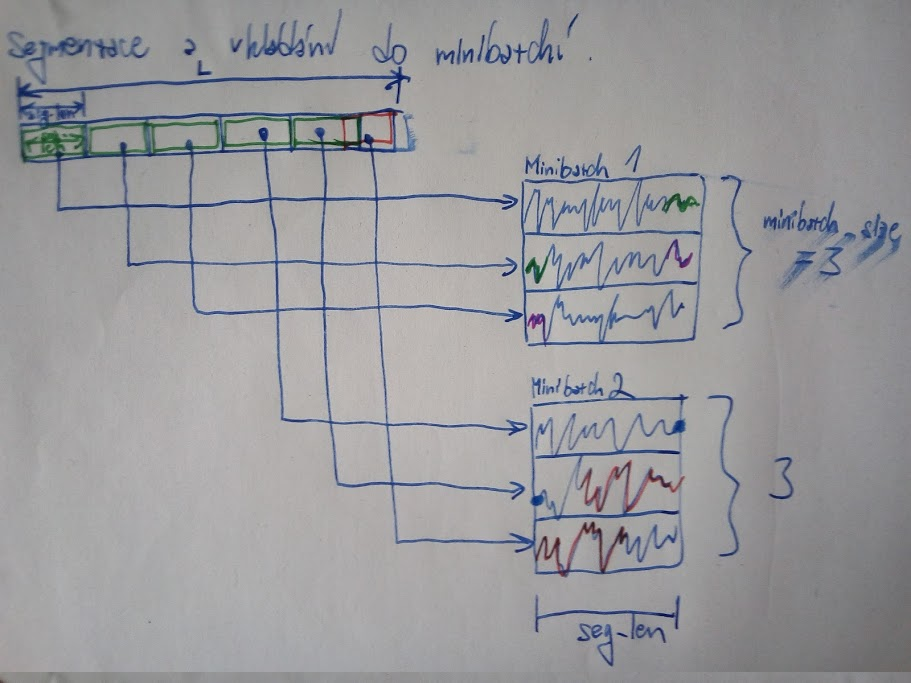
\includegraphics[scale=0.30]{obrazky-figures/minibatch_segmentace.jpg}
    \caption{\label{fig:minibatch_segmentace}Dělení nahrávky na segmenty o délce \textbf{segment\_len} a jejich následné vkládání do minibatche. Lze si všimnout, že pokud poslední segment není dostatečně dlouhý, tak se vezme od konce nahrávky a jeho počáteční vzorky budou duplicitní s posledními vzorky předešlého segmentu}
\end{figure}

\begin{figure}[H]
    \centering
    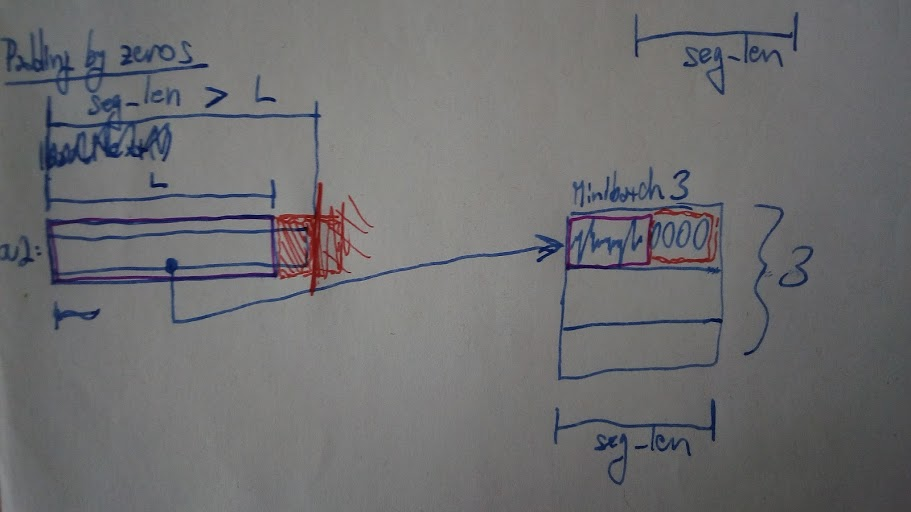
\includegraphics[scale=0.30]{obrazky-figures/minibatch_segmentace_padding.jpg}
    \caption{\label{fig:segmentace_padding}Je--li zpracovávána nahrávka, jejíž délka je kratší než je délka segmentu, je tento segment doplněn z prava nulami do požadované délky}
\end{figure}

\todo{mozna tento odstavec jeste nejak upravit a doplnit obrazek kde je nacitani asi 3 audio nahravek}
Algoritmus \ref{alg:segmentace_nahravek} a obrázek \ref{fig:generovani_segmentu} zobrazují proces segmentace. Funkce $\texttt{segmentGenerator()}$, která slouží jako generátor, pracuje současně se třemi nahrávkami -- se směsí dvou mluvčích, s nahrávkou prvního mluvčího a s nahrávkou druhého mluvčího, které jsou do atributů $\texttt{current\_mixture}$, $\texttt{current\_source1}$ a $\texttt{current\_source2}$ třídy $\texttt{SegmentDataset}$ nahrávány funkcí $\texttt{loadNextAudio()}$ poté, co z předchozí trojice nahrávek již nelze vygenerovat další segmenty.

\bigskip

\begin{algorithm}[H]
\LinesNumbered
\SetKwProg{Fn}{Function}{ is}{end}
 \Fn{segmentGenerator() : int[]}{
	 $\texttt{s1\_segment} = \texttt{[]}$\;
	 $\texttt{segptr} = \texttt{0}$\;
	 \While{$\texttt{je dostupná další trojice nahrávek}$}{
		\eIf{$\texttt{current\_mixture\_len} < \texttt{SEGMENT\_LENGTH}$}{
			\tcc{aktuální nahrávka je kratší než délka segmentu}
			$\texttt{s1\_segment} = \texttt{current\_source1[:]}$\;
			$\texttt{yield s1\_segment}$\;
		}{
			\eIf{$\texttt{segptr} + \texttt{SEGMENT\_LENGTH} < \texttt{current\_mixture\_len}$}{
				\tcc{z aktuální nahrávky vzít segment}				
				$\texttt{s1\_segment} = \texttt{current\_source1[(segptr+SEGMENT\_LENGTH)]}$\;
				$\texttt{segptr} += \texttt{SEGMENT\_LENGTH}$\;
				$\texttt{yield s1\_segment}$\;
			}{
				\tcc{nelze již načíst celý segment, takže se vezme od konce}
				$\texttt{start\_index} = \texttt{(current\_mixture\_len - SEGMENT\_LENGTH)}$\;
				$\texttt{s1\_segment} = \texttt{current\_source1[start\_index:current\_mixture\_len]}$\;
				$\texttt{yield s1\_segment}$\;
			}
		}
	}
 }
 \caption{\label{alg:segmentace_nahravek}Algoritmus segmenace nahrávek používá výhody python generátoru, který, narozdíl od běžných funkcí, po vrácení hodnoty příkazem \texttt{yield} neztrácí svůj vnitřní stav a při jeho dalším zavolání pokračuje tam, kde skončil. V uvedeném příkladě je znázorněna pouze segmentace nahrávky jednoho mluvčího, ale analogicky se segmentují i nahrávky směsi mluvčích a nahrávky druhého mluvčího}
\end{algorithm}


\begin{figure}[H]
    \centering
    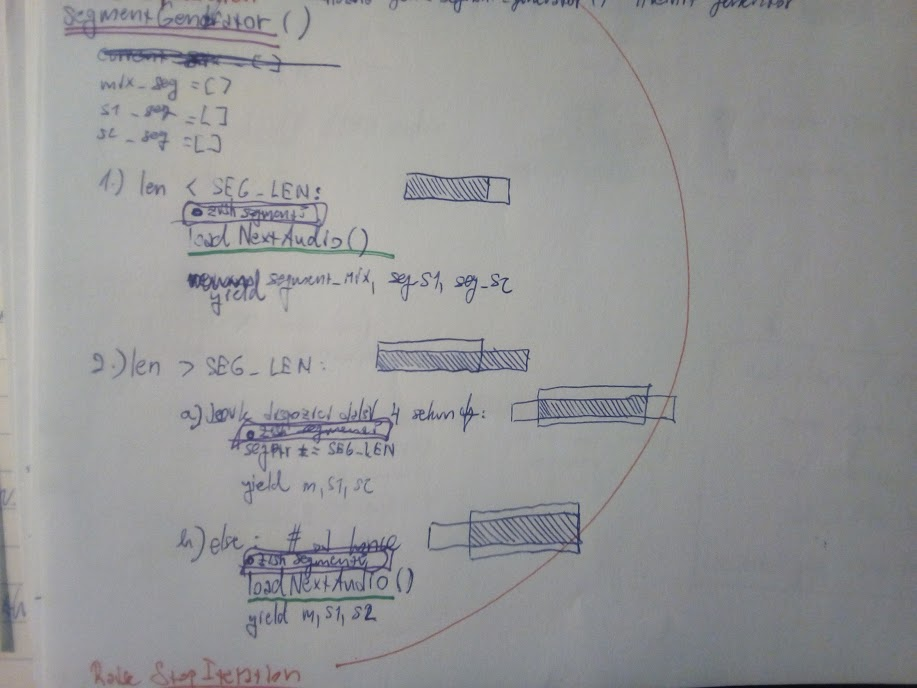
\includegraphics[scale=0.30]{obrazky-figures/segmentation.jpg}
    \caption{\label{fig:generovani_segmentu}Způsob segmentace nahrávek}
\end{figure}


Kód segmentace také umožňuje určit délku, o kterou se segmenty budou překrývat. Této funkcionality je docíleno zavedením proměnné \texttt{overlap}, která obsahuje délku překrytí a při segmentaci je od proměnné \texttt{offset}, který určuje začátek následujícího segmentu, tato hodnota odečtena, jak ukazuje obrázek \ref{fig:segment_overlap}. Při trénování je překrytí nulové, protože by to zvýšilo počet trénovacích dat jejich částečnou duplikací, což by negativně ovlivnilo délku trénování.

\begin{figure}[H]
    \centering
    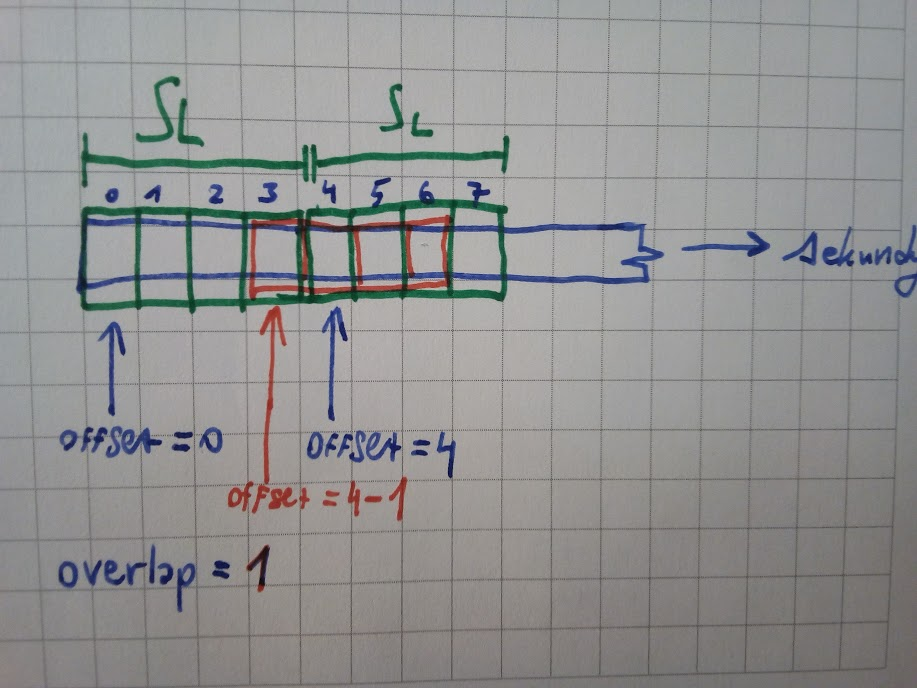
\includegraphics[scale=0.25]{obrazky-figures/segment_overlap.jpg}
    \caption{\label{fig:segment_overlap}Segmentace nahrávek s nenulovým překrytím}
\end{figure}

%------------------
\section{Výpočet hodnoty loss za pomoci si--snr}
\todo{popsat implementaci sisnr a vypocet loss za pomoci cross vypoctu, obrazek}

\begin{figure}[H]
    \centering
    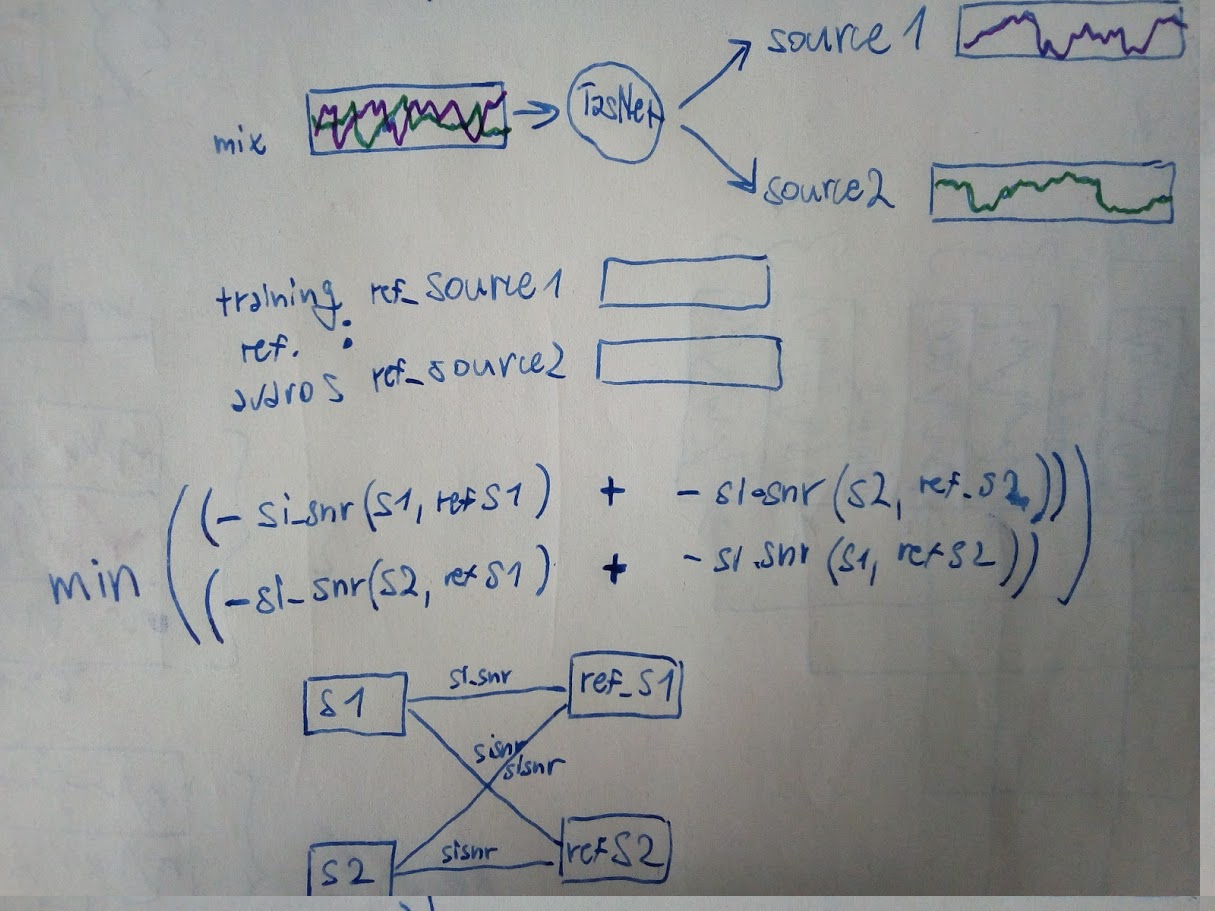
\includegraphics[scale=0.25]{obrazky-figures/sisnr_cross_calculation.jpg}
    \caption{\label{fig:implementace_loss_sisnr} Implementace a zjištění správné pozice korespondujících nahrávek pro výpočet hodnoty loss}
\end{figure}

%------------------
%------------------


\section{Pomocné skripty}
Během implementace se vyskytla potřeba zjednodušit si některé repetetivní úkony a jelikož upřednostňuji práci z terminálu, tak jsem si pro ně naprogramoval několik skriptů za použití jazyků python3 a bash. 

Skript \textbf{\textit{gupload.sh}} pro odesílání zdrojových souborů na \textit{Google Drive}\footnote{\url{https://www.google.com/drive/}}, ze kterého \textit{Google Colab}\footnote{\url{https://colab.research.google.com/notebooks/intro.ipynb}} načítá data a kód, který lze následně po částech spouštět z grafického rozhraní. K interakci s Google Drive jsem použil nástroj \textit{rclone}\footnote{\url{https://rclone.org/}}, který nabízí mnoho operací pro vzdálenou práci s Google Drive z terminálu. S pomocí \textit{rclone} lze stahovat či nahrávat data, vzdáleně měnit adresářovou strukturu, mazat, vytvářet a upravovat soubory a podobně. 

Skript \textbf{\textit{gdownload.sh}} je určený pro snadné stahování dat z Google Drive. Stejně jako předchozí skript, používá operace poskytované nástrojem rsync. Při zavolání stáhne adresář obsahující data z posledního trénování, nebo adresář, jehož název je předán jako argument skriptu v přikazové řádce.   
Stažený adresář obsahuje checkpointy, soubory obsahující výstup trénování, soubor obsahující dvojice hodnot $[zpracováno_nahrávek, loss]$, které lze jednoduše vykreslit do grafu, a nakonec soubor s výsledky testování obsahující hodnoty metrik pro testovaný checkpoint.

Dále jsem vytvořil několik jednoduchých skriptů pro rychlé spuštění trénování a testování modelu s různými přednastavenými parametry. Bylo tak možno mít mezi skripty rozdílné cesty k adresářům pro účely trénování a ladění chyb nebo třeba nastavení času, po kterém se proces má sám ukončit. Pro spuštění trénování modelu tak lze zavolat skript \textbf{\textit{nntrain.sh}}, pro testování skript \textbf{\textit{nntest.sh}} a pro inferenci (separaci mluvčích na předané nahrávce) skript \textbf{\textit{nninference.sh}}.


\bigskip

Implementace samotného modelu ve frameworku pytorch nebyla náročná. Vzhledem k netriviálnímu úkolu jsem musel implementovat některé části, jako třeba segmentace nahrávek, sám. To přineslo mnoho potíží při odstraňování chyb v samotném modelu. Síť jsem prvně trénoval a ladil na CPU svého notebooku, takže probíhalo velmi pomalu (v řádu desítek hodin i při nízké velikosti modelu), a některé chyby se objevily až v průběhu trénování nebo dokonce na jeho konci. Situaci razantně zlepšil přechod na Google Colab, kde jsem síť trénoval na poskytovaných GPU a trénování tak zabralo \todo{"pouze" (opravit uvozovky)} několik hodin, takže se případná chyba objevila dříve, ale i přesto mi lazení sítě zabralo mnoho času. Pro další usnadnění samotné implementace jsem vytvořil několik skriptů, které mi usnadnily spouštění a lazení sítě.

%----------------------------------------------------------------------------------------------------------------------------------------------------------------------


\chapter{Experimenty a vyhodnocení}
\label{experimenty}
- trenovani s~ruznymi hyperparametry, uspesnost a tabulky s~hyper parametry a dosazenymi vysledky a hodnotami sisnr, sdr atd.
- model size comparison.
- porovnani s~vysledky ze studie
- obrazky separovanych mluvcich - signalu.
- spektra
- grafy trenovani loss a vysledkuu.
- pametova narocnost modelu


Neuronové sítě představují mocný nástroj mnoha využití, který ale musí být naučen, jak danou činost provádět. Trénování sítí je výpočetně náročný úkol, jehož náročnost se, krom dalších parametrů, může lišit v závislosti na velikosti datasetu a sítě. Obecně čím větší dataset a rozměr sítě, tím déle trénování trvá. Je proto podstatné, na jakém stroji je síť učena a od toho se odvíjí čas trénování.

Po dostatečném natrénování probíhá vyhodnocení sítě. Výsledky trénování jsou měřeny metrikami, které se volí na základě problému, který se síť učila řešit. Výsledky testování sítě jsou následně porovnávány v závislosti na velikosti daného modelu. Velikost modelu je ovlivněna hyper--parametry, které určují například počet vrstev sítě, velikost segmentace a další vlastnosti.

Cílem experimentů je zjistit, které z hyper--parametrů mají největší vliv na kvalitu separace a tedy na výsledky vyhodnocení, a jak moc lze model zmenšit, aby stále dával dostatečně dobré výsledky separace mluvčích. Tato kvalita je měřena primárně metrikami STOI, SI--SNR a PESQ, které byly popsány v kapitole \ref{separace}.
\todo{ref na zdroje u metrik}


\section{Dataset}
Dataset je množina dat, na kterých je síť učena a testována. Dataset se dá rozdělit na 3 podmnožiny, které jsou navzájem exkluzivní. Trénovací dataset je určen k trénování sítě a bývá největší. Validační dataset se prochází po zpracování trénovacího datasetu v průběhu trénování a slouží pro ověření, že hodnota loss na dosud neviděných datech stále klesá a nedochází tak k přetrénování. Při zpracování tohoto datasetu je síti zabráněno v učení. Poslední je testovací dataset, na kterém probíhá vyhodnocení sítě, tedy výpočet hodnot jednotlivých metrik. 

Trénování a vyhodnocení modelu proběhlo na množině jednokanálových nahrávek směsí dvou mluvčích. Množina byla vygenerována náhodným výběrem různých mluvčích z~Wall Street Journal (WSJ0) a vytvořením směsi mluvčích z těchto dvou náhodně vybraných nahrávek. Celková délka trénovacích dat je přes 10 hodin a přes 6 hodin validačních dat. Nahrávky jsou převzorkovány na 8kHz a během trénování zarovnány na zero means a jednotkovou varianci \todo{[studie str 5 Dataset][49 - ze studie odkaz na script na generovani a popis na netu]}.

\begin{figure}[H]
    \centering
    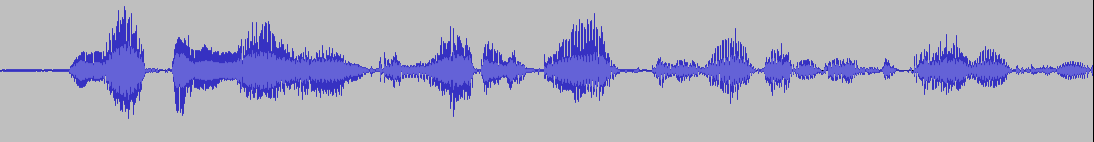
\includegraphics[scale=0.35]{obrazky-figures/dataset-mix.png}
    \caption{\label{fig:ref-mixture}Ukázka nahrávky směsi dvou mluvčích}
\end{figure}

\begin{figure}[H]
    \centering
    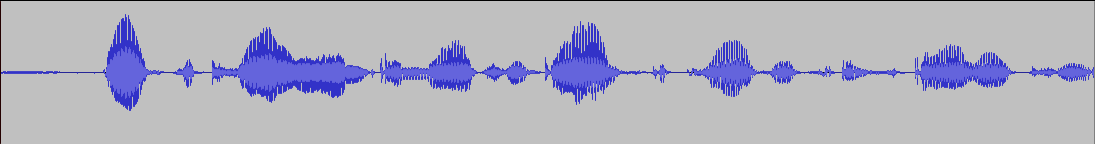
\includegraphics[scale=0.35]{obrazky-figures/dataset-s1.png}
    \caption{\label{fig:ref-s1}První mluvčí ze směsi}
\end{figure}

\begin{figure}[H]
    \centering
    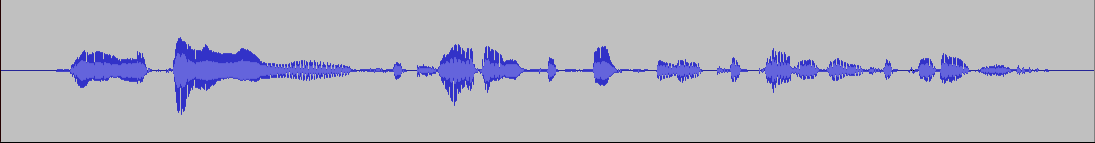
\includegraphics[scale=0.35]{obrazky-figures/dataset-s2.png}
    \caption{\label{fig:ref-s2}Druhý mluvčí ze směsi}
\end{figure}

Lze si všimnout, že sečtením signálů separovaných mluvčích na obrázku \ref{fig:ref-s1} a \ref{fig:ref-s2} dostaneme přesně signál směsi, což lze vyjádřit vztahem

\begin{equation}
  x[t] = \sum_{i=1}^C s_i[t]
\end{equation}
, kde $x[t] \in \mathbb{R}^{1 \times T}$ je diskrétní signál směsi a $s_i[t] \in \mathbb{R}^{1 \times T}$, kde $i = 1,\ldots,C$, je jeden z~$C$ zdrojů[cite studie str3 vlevo]. 

\todo{doplnit info o~zero means a jendotkove varianci}


%------------------------------------------------------------------------------


\section{Průběh trénování}
\todo{miniÚvod - konkretni hyperparams, vykon a cas trenovani, seg--len, bylo natrenovano nekolik modelu ... konkretni hyperparams, vykon a cas trenovani, seg--len}.
Bylo natrénováno několik, různě velkých modelů, které se lišily velikostí jejich hyper--parametrů, konkrétně počtem konvolučních bloků, počtem jejich opakování a velikostí segmentů zpracovávaných nahrávek z datasetu. 

\todo{https://www.tablesgenerator.com/}.

\begin{table}[hbt]
\centering
\caption{Hodnoty hyperparametrů trénovaných sítí a jejich přesnost}
\label{hodnoty}
\begin{tabular}{|l|c|c|c|}
\hline
 & X & R & segment length  \\
 &  &  & sisnr  \\ \hline
2 & 2 & 4 & 8.3 \\ \hline
3 & 2 & 4& 9.45 \\ \hline
4 & 3 & 4 & 10.2 \\ \hline
8 & 4 & 2 & 13.6 \\ \hline
\end{tabular}
\end{table}


\begin{figure}[H]
    \centering
    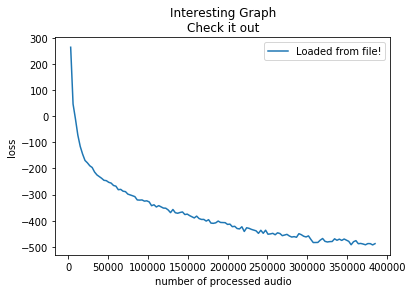
\includegraphics[scale=0.55]{obrazky-figures/some-loss.png}
    \caption{\label{fig:somelossTODO}Příklad grafu loss hodnoty během učení}
\end{figure}

\begin{figure}[H]
    \centering
    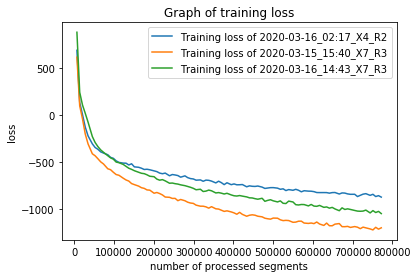
\includegraphics[scale=0.55]{obrazky-figures/loss_triple.png}
    \caption{\label{fig:somelossTODO2}Hodnota loss při trénování modelů s~různou velikostí hyperparametrů}
\end{figure}


%------------------------------------------------------------------------------

\section{Experimenty s modely}
\todo{rozdelit tabulku podle HP a spis mensi tabulku ukazujici vysledku pro konkretni hyper parametry.
experimenty:
sisnr, reportovat ruzne metriky - stoi, pesq, prozkoumat hyper parametry a jak ktere jsou dulezite. Kdyz budu zmensovat sit tak jak se bude zhorsovat.}

\todo{miniÚvod}
Pro vyhodnocení úspěšnosti a kvality modelů byly použity metriky si--snr vyjadřující poměr XXX, pesq říkající YYY a stoi vyjadřující ZZZ \todo{mozna ref}.  

\subsection{Vliv hyper--parametru X}
\todo{zmensovani a zvetsovani X, vysledky testovani, loss pripadne nejake fajnove grafy porovnani vysledky mezi jednotlivymi X, obrazky, grafy}

\subsection{Vliv hyper--parametru R}
\todo{zmensovani a zvetsovani Y, vysledky testovani, loss pripadne nejake fajnove grafy porovnani vysledky mezi jednotlivymi Y, obrazky, grafy}

\subsection{Vliv hyper--parametru délka--segmentu}
\todo{zmensovani a zvetsovani SL, vysledky testovani, loss pripadne nejake fajnove grafy porovnani vysledky mezi jednotlivymi SL, obrazky, grafy}

\subsection{Vyhodnocení a porovnání modelů}
\todo{shrnuti a porovnani jednotlivych zmen mezi sebou komplexne. Pripadne porovnani vysledku s ref studii, obrazky, grafy}




\section{Možná rozšíření a navrhnutá vylepšení}
- variabilnější dataset, mikrofony, šum a bordel prostředí
- separace více mluvčích
- hlučné prostředí
- identifikace konkrétního řečníka
- realtime separace

%----------------------------------------------------------------------------------------------------------------------------------------------------------------------
%----------------------------------------------------------------------------------------------------------------------------------------------------------------------

\chapter{Závěr}
\label{zaver}
\todo{co jak dopadlo, vysledky a vyhodnoceni velikosti modelu a jaky byl nejlepsi}

Cílem práce bylo implementovat síť podle architektury TasNet pro separaci mluvčích v~časové doméně a porovnat vliv velikosti sítě na kvalitu separace. Síť byla implementována za pomoci frameworku pytorch a jazyku python a natrénována na datasetu obsahujícím jednokanálové směsi dvou mluvčích. Trénování proběhlo na \todo{X} modelech, které se od sebe lišily počtem opakujících se konvolučních bloků, velikostí časové dilatace a délkou vstupních segmentů směsí. Pro účel vyhodnocení modelů byla použita metrika si-snr, která udává poměr chtěného signálu ku šumu na pozadí, tedy obecně kvalitu separace. 

Experimenty ukázaly, že během testování nejlépe dopadla síť, která měla 8 konvolučních bloků po 4 opakováních, s~délkou vstupního segmentu $L=2$ sekundy. Tento model dosáhl po 100 epochách trénování hodnoty až \todo{13,4} a tím se stal nejúspěšnějším modelem. Při fyzickém poslechu separovaných nahrávek bychom neslyšeli téměř žádný náznak druhého mluvčího. Oproti tomu, nejméně přesný model měl pouze 4 konvoluční bloky, 2 opakování a při délce segmentů $L=4$ sekundy dosahoval hodnoty SDR pouze \todo{9.2}.

Zkoušel jsem separovat také nahrávky, které byly úplně mimo dataset, ale výsledek se nedá hodnotit jako úspěšný, jelikož hraje velkou roli prostředí, mikrofon, šum v~pozadí a další vlivy, na které byla neuronová síť naučena. Tento problém by se dal překonat rozšířením trénovacího datasetu o~větší škálu nahrávek mluvčích, které by byly pořízeny z~různých zařízení v~různě rušném prostředí.

\todo{Doplnit ještě neco eh}
Mozna.



  \fi
  
  % Kompilace po částech (viz výše, nutno odkomentovat)
  % Compilation piecewise (see above, it is necessary to uncomment it)
  %\subfile{projekt-01-uvod-introduction}
  % ...
  %\subfile{chapters/projekt-05-conclusion}


  % Pouzita literatura / Bibliography
  % ----------------------------------------------
\ifslovak
  \makeatletter
  \def\@openbib@code{\addcontentsline{toc}{chapter}{Literatúra}}
  \makeatother
  \bibliographystyle{bib-styles/Pysny/skplain}
\else
  \ifczech
    \makeatletter
    \def\@openbib@code{\addcontentsline{toc}{chapter}{Literatura}}
    \makeatother
    \bibliographystyle{bib-styles/Pysny/czplain}
  \else 
    \makeatletter
    \def\@openbib@code{\addcontentsline{toc}{chapter}{Bibliography}}
    \makeatother
    \bibliographystyle{bib-styles/Pysny/enplain}
  %  \bibliographystyle{alpha}
  \fi
\fi
  \begin{flushleft}
  \bibliography{projekt-20-literatura-bibliography}
  \end{flushleft}

  % vynechani stranky v oboustrannem rezimu
  % Skip the page in the two-sided mode
  \iftwoside
    \cleardoublepage
  \fi

  % Prilohy / Appendices
  % ---------------------------------------------
  \appendix
\ifczech
  \renewcommand{\appendixpagename}{Přílohy}
  \renewcommand{\appendixtocname}{Přílohy}
  \renewcommand{\appendixname}{Příloha}
\fi
\ifslovak
  \renewcommand{\appendixpagename}{Prílohy}
  \renewcommand{\appendixtocname}{Prílohy}
  \renewcommand{\appendixname}{Príloha}
\fi
%  \appendixpage

% vynechani stranky v oboustrannem rezimu
% Skip the page in the two-sided mode
%\iftwoside
%  \cleardoublepage
%\fi
  
\ifslovak
%  \section*{Zoznam príloh}
%  \addcontentsline{toc}{section}{Zoznam príloh}
\else
  \ifczech
%    \section*{Seznam příloh}
%    \addcontentsline{toc}{section}{Seznam příloh}
  \else
%    \section*{List of Appendices}
%    \addcontentsline{toc}{section}{List of Appendices}
  \fi
\fi
  \startcontents[chapters]
  \setlength{\parskip}{0pt} 
  % seznam příloh / list of appendices
  % \printcontents[chapters]{l}{0}{\setcounter{tocdepth}{2}}
  
  \ifODSAZ
    \setlength{\parskip}{0.5\bigskipamount}
  \else
    \setlength{\parskip}{0pt}
  \fi
  
  % vynechani stranky v oboustrannem rezimu
  \iftwoside
    \cleardoublepage
  \fi
  
  % Přílohy / Appendices
  \ifenglish
    % Tento soubor nahraďte vlastním souborem s přílohami (nadpisy níže jsou pouze pro příklad)
% This file should be replaced with your file with an appendices (headings below are examples only)

% Umístění obsahu paměťového média do příloh je vhodné konzultovat s vedoucím
% Placing of table of contents of the memory media here should be consulted with a supervisor
%\chapter{Obsah přiloženého paměťového média}

%\chapter{Manuál} % Manual

%\chapter{Konfigurační soubor} % Configuration file

%\chapter{RelaxNG Schéma konfiguračního souboru} % Scheme of RelaxNG configuration file

%\chapter{Plakat} % poster

\chapter{How to use this template}
\label{jak}

This chapter describes individual parts of the template, followed by a brief instructions on how to use it. If you have any questions, comments etc, feel free to email them to me at sablona@fit.vutbr.cz.

\section*{Template parts description}

Once you extract the template, you will find the following files and directories:
\begin{DESCRIPTION}
  \item [bib-styles] Literature styles (see below).
  \item [obrazky-figures] Directory for your images. Currently contains placeholder.pdf (a.k.a TODO image -- see below) and image keep-calm.png to demonstrate inserting raster images (you don't submit these images with your thesis). It is advised to use shorter directory name, so that it is only in your chosen language.
  \item [template-fig] Template images (BUT logo).
  \item [fitthesis.cls] Template (design definition).
  \item [Makefile] Makefile used to compile the project, count standard pages etc. (see below).
  \item [projekt-01-kapitoly-chapters.tex] File for Your text (replace it's contents).
  \item [projekt-20-literatura-bibliography.bib] Reference list (see below).
  \item [projekt-30-prilohy-appendices.tex] File for your enclosures (replace it's contents).
  \item [projekt.tex] Main project file -- definitions of formal parts.
\end{DESCRIPTION}

Eng. Martínek provided the default literatuter style (czechiso), and english version (englishiso) is it's slightly modified translation. It differs from the standard in some aspects, but it is accepted at FIT for a long time now. Alternatively, you can use a style provided by Eng. Radim Loskot or Eng. Radek Pyšný\footnote{BP Ing. Radka Pyšného \url{http://www.fit.vutbr.cz/study/DP/BP.php?id=7848}}. Alternative styles have certain improvements, but they weren't yet properly tested by a larger quantity of users. They can be considered beta versions for those interested in making their thesis perfect, that comes with the need to study proper citation formatting.

Aside from compilation to PDF, the Makefile also offers additional functions:
\begin{itemize}
  \item rename files (see below),
  \item count standard pages,
  \item run a wave that adds unbreakable spaces,
  \item compress (zip) the result, ready to be sent to your supervisor and checked (make sure that all the files you've added are included, if not, add them manually).
\end{itemize}

Keep in mind that the wave is not perfect. You always need to check whether or not there is something inappropriate at the end of a line manually -- see Online language handbook\footnote{Internetová jazyková příručka \url{http://prirucka.ujc.cas.cz/?id=880}}.

% Některá typografická doporučení uvádí, že na koncích řádků nevypadají dobře ani jednoslabičné spojky a předložky jako \uv{do}, \uv{od}, \uv{po} apod. Obdobná pravidla se uplatňují také v angličtině -- viz např. článek Run Ragged\footnote{Run Ragged\url{https://24ways.org/2013/run-ragged/}}, dle kterého na koncích řádků nemají být předložky, pomlčka ani krátká slova (2--3 písmena), dva následující řádky nemají končit čárkou a nemají se zalamovat zvýrazněné fráze z 2 -- 3 slov.

\paragraph {Pay attention to page numbering!} If the table of contents is 2 pages long and the second page contains only \uv{Enclosures} and \uv{List of enclosures} (but there is no enclosure), the page numbering is changed by 1 (table of contents and contents \uv{mismatch}). The same thing happens if the second or third page contains only \uv{References} and there's a chance that this can occur in other situations too. There are multiple solutions to this (from editing the table of contents, setting the page counter all the way to more sophisticated methods). \textbf{Check the page numbering before you submit your thesis!}

\section*{Recommendations for working with the template}

\begin{enumerate}
  \item \textbf{Make sure you have the latest version of template.} If you have a template from last year, there should be a newer version (updated information, fixed errors etc.) available at the faculty or study advisor web pages.
  \item \textbf{Choose a language}, that you want to use for your technical report (czech, slovak or english) and consult your supervisor about your choice (unless it was agreed upon in advance). If your language of choice is not czech, set the respective template parameter in file projekt.tex (e.g.: \verb|documentclass[english]{fitthesis}| and translate the declaration and acknowledgement to english or slovak).
  \item \textbf{Rename the files.} When you extract the files, there should be a file named projekt.tex. If you compile it, it will create a PDF with technical report named projekt.pdf. If multiple students send their supervisor projekt.pdf to have it checked, they have to rename them. For that reason, it is advised to rename the file so that it contains your login and (if needed, abbreviated) work topic. Avoid using spaces, diacritic and special symbols. An appropriate name for your file can look like this: \uv{xlogin00-Cleaning-and-extraction-of-text.tex}. You can use the included Makefile to rename it:
\begin{verbatim}
make rename NAME=xlogin00-Cleaning-and-extraction-of-text
\end{verbatim}
  \item Fill in the required information in file, that was originally named projekt.text, that means type, year (of submission), thesis title, author's name, department (according to specification), supervisor's titles and name, abstract, keywords and other formal requirements.
  \item Replace the contents of thesis chapters, references and enclosures files with the contents of your technical report. Individual enclosures or thesis chapters can be saved to separate files -- if you choose this approach, it is advised to comply with the file naming convention, and the number will be followed by the chapter title.
  \item If you don't need enclosures, comment the respective part in projekt.tex and erase everything from the corresponding file or delete it. Don't try to come up with an aimless enclosures just to have something in that file. An appropriate enclosure can be the contents of included memory medium.
  \item Save the scanned specification to specification.pdf and allow it to be inserted into the thesis project using the (\verb|documentclass[zadani]{fitthesis}|) template parameter in projekt.tex.
  \item If you don't want to print references in color (red contents -- i cannot recommend this without consulting your supervisor), you'll need to create a second PDF for printing and set the template printing parameter:\\ (\verb|documentclass[english,zadani,print]{fitthesis}|). Colored logo must not be printed in black and white.
  \item The binder templace where the thesis will be typeset can be generated in faculty IS at specification. Can be enabled for dissertation using the \tt cover \rm parameter in template.
  \item Don't forget that source files and (both versions) PDF has to be on a CD or other medium included in the technical report.
\end{enumerate}

\subsection*{Instructions for double-sided printing}
\begin{itemize}
\item \textbf{It is advised to consult your supervisor about double-sided printing.}
\item If you used double-sided printing for your thesis and it's thickness is smaller than the thickness of the binder, it doesn't look too good.
\item Enabled using the following template parameter:\\ \verb|\documentclass[twoside]{fitthesis}|
\item After printing a double-sided sheet, make sure that the canon of page construction is in the same position on both pages. Inferior printers with duplex printing unit usually cause a shift by 1--3 mm. This can be solved with some printers. Print the odd pages first, put them back into the same tray and print the even pages.
\item Leave a blank page after title page, table of contents, references, list of enclosures and other lists to make sure that the following part starts on an odd page (\textbackslash cleardoublepage).
\item Check the final result thoroughly.
\end{itemize}


\subsection*{Useful tools}
\label{nastroje}

The following list is not a list of all useful tools. If you have experience with a certain tool, feel free to use it. However, if you don't know which tool to choose, consider the ones listed below:

\begin{description}
	\item[\href{http://miktex.org/download}{MikTeX}] \LaTeX{} for Windows -- a distribution with simple installation and great automated package downloading. MikTeX even has it's own editor, but I highly recommend TeXstudio.
	\item[\href{http://texstudio.sourceforge.net/}{TeXstudio}] Portable opensource GUI for \LaTeX{}. Ctrl+click switches between source text and PDF. Integrated spell checker\footnote{Spell checker for czech version can be installed from \url{https://extensions.openoffice.org/de/project/czech-dictionary-pack-ceske-slovniky-cs-cz}}, syntax highlighter etc. To use this tool, you need to first install MikTeX or another \LaTeX{} distribution.
    \item[\href{http://www.winedt.com/}{WinEdt}] A good combination for Windows is WinEdt + MiKTeX. WinEdt is a GUI for Windows, and if you want to use it, you need to first install \href{http://miktex.org/download}{MikTeX} or \href{http://www.tug.org/texlive/}{TeX Live}.
    \item[\href{http://kile.sourceforge.net/}{Kile}] Editor for KDE (Linux) desktop environment. Real-time preview. To use this tool, you need to have \href{http://www.tug.org/texlive/}{TeX Live} and Okular installed.
	\item[\href{http://jabref.sourceforge.net/download.php}{JabRef}] Neat and simple Java program for bibliography (references) file management. No need to learn anything -- provides a simple window and a form for entry editing.
	\item[\href{https://inkscape.org/en/download/}{InkScape}] Portable opensource vector graphic (SVG and PDF) editor. Excellent tool to use to create images for technical text. Difficult to master, but the results are worth it.
	\item[\href{https://git-scm.com/}{GIT}] Great tool for teamwork when it comes to projects, but can be incredibly useful even to a single author. Simple version control system, backup options and transfer between multiple computers.
	\item[\href{http://www.overleaf.com/}{Overleaf}] Online \LaTeX{} tool. A real-time compilation of source text that allows for simple collaboration (supervisor can continuously keep an eye on the progress made), move to a place in source file just by clicking in the PDF preview, spell checker etc. There are some limitations to what you can do if you want to use it for free (some people are comfortable with it for dissertation, others can run into it while they write a~bachelor's thesis) and it is rather slow for long texts. FIT has a license for supervisors and if a~student encounters an issue, it can be solved with the help of their supervisor.
\end{description}

Note: Overleaf does not use template Makefile -- to get compilation to work, you need to right-click \tt projekt.tex \rm and select \uv{Set as Main File}.

\chapter{Writing english texts}
\label{anglicky}
This chapter is taken from web pages of Jan Černocký \cite{CernockyEnglish}.

A lot of people write their technical reports in english (which is good!), but they make a~lot of unnecesary mistakes (which is bad!). I'm not an english export myself, but I've been using this language for a while now to write, read and even communicate -- this chapter contains a handful of important things. If you want to be certain that your thesis or article is 100\,\% correct, your best bet is to hire a native speaker (preferably someone who is technically capable and understands what you write about \ldots).


\section*{In general}

\begin{itemize}
  \item{Before you jump into it head first, I suggest you read a handful of technical articles written in english and try to remember or preferably understand how you should approach writing one yourself.}
  \item{Always use a spell checking tools -- built in tools in Word, or in OpenOffice. If you work on Linux, I suggest you use ISPELL. Some spell checking (I think it's the one in PSPad) are not very good and ignore a lot of mistakes.}
  \item{Use grammer checking tools. I'm not entirely sure if there is one available for Linux, but the one in Word is fairly decent and if it underlines anything with green color, it's probably wrong. You can even copy and paste Latex source code here, fix any and all grammar errors and save it as a clean text again. If you use vim, there's a~built in grammar checking tool too, and it's capable of detecting typos and errors in basic grammar. Write this in the first line of your thesis tex file:
  \begin{verbatim}
    % vim:spelllang=en_us:spell
  \end{verbatim}
  (alternatively \texttt{en\_gb} for OED english) \textit{Editor's note:} There is a very good online tool Grammarly\footnote{\url{https://www.grammarly.com/}}, with free basic version.
  }
  \item{Online dictionaries are good, but don't rely on them in every situation. Usually you get multiple choices and not all of them are correct for the given context.}
  \item{\begin{samepage}You can probably figure out what the correct option is by looking each option up and seeing the context in which they're used, example given: ``advantage/privilege/facility of approach''. Online dictionaries give you a handful of results. Look them up one by one using google search:
  \begin{verbatim}
    "advantage of this approach" 1100000 hits
    "privilege of this approach" 6 hits
    "facility of this approach"  16 hits
  \end{verbatim}
  I'm not saying it's 100\,\% correct, but at least you have something to go on. This can be used to find the correct connectives (e.g. ``among two cases'' or ``between two cases''?)\end{samepage}}
\end{itemize}

\section*{SVOMPT and concord}

The structure of an english sentence is SVOPMT: SUBJECT VERB OBJECT MANNER PLACE TIME and there's no other way around it. It is not a flexible structure. There are possibly exceptions in things like a theater play, where something needs to be emphasized. Subject must be present in every single single sentence, people tend to forget as some languages have a sentence structure where the subject can be implicit and not mentioned. SVOMPT applies to dependent clauses too!
\begin{verbatim}
  BAD: We have shown that is faster than the other function.
  GOOD: We have shown that it is faster than the other function.
\end{verbatim}

\noindent Concord or grammatical agreement between two words in a sentence -- it sounds silly, but people make countless mistakes here.

\begin{verbatim}
  he has
  the users have
  people were
\end{verbatim}

\section*{Articles}

Articles in english are a nightmare and almost all of us fail to use them correctly. The basic rule is, that if there's a particular noun, it's preceeded by ``the''. Definite articles must be in following phrases:
\begin{verbatim}
  the first, the second, ...
  the last
  the most (superlatives and adverbs) ...
  the whole
  the following
  the figure, the table.
  the left, the right - on the left pannel, from the left to the right ...
\end{verbatim}

\noindent On the contrary, there can't be an article when you're referring to a specific figure, chapter, etc.
\begin{verbatim}
  in Figure 3.2
  in Chapter 7
  in Table 6.4
\end{verbatim}

\begin{samepage}
\noindent The use of ``a'' and ``an'' is based on the pronounciation, rather than how the word is written:
\begin{verbatim}
  an HMM
  an XML
  a universal model
  a user
\end{verbatim}
\end{samepage}

\section*{Verbs}

Passive voice can be tricky -- regular verbs are usually not a problem, irregular verbs however are a common source of errors, typically
\begin{verbatim}
  packet was sent (rather than send)
  approach was chosen (rather than choosed)
\end{verbatim}
\noindent \ldots most of the time, the spell checker will correct it, but it's not guaranteed.

Tenses are a mess at times. If something just is in general, use present tense. If you did something, use past tense. If you got results that already exist and you just discuss them, use present tense. Try to avoid complicated tenses such as present perfect or worse past perfect if you're not 100\,\% sure.
\begin{verbatim}
  JFA is a technique that works for everyone in speaker recognition.
  We implemented it according to Kenny's recipe in \cite{Kenny}.
  12000 segments from NIST SRE 2006 were processed. When compared
  with a GMM baseline, the results are completely bad.
\end{verbatim}

\section*{Sentence length and structure}

\begin{itemize}
  \item{Try to write shorter sentences. If you sentence is 5 lines long, it's probably a pain to read, if it can even be done.}
  \item{Comma is a powerful tool and you should use it for your sentence structure. Use a~comma to seperate the initial dependent clause from the main independent clause. Sometimes it is appropriate to put a comma just before ``and'' (unlike other languages)!}
\end{itemize}
\begin{verbatim}
  In this chapter, we will investigate into ...
  The first technique did not work, the second did not work as well,
  and the third one also did not work.
\end{verbatim}

\section*{The specifics of a technical text}

When writing a technical text, don't use common phrases such as
\begin{verbatim}
  he's
  gonna
  Petr's working on ...
\end{verbatim}
\noindent and others. The only tolerated thing is ``doesn't'', but you can never go wrong with ``does not''.

\begin{samepage}
\noindent Technical texts utilize passive voice a lot more than active voice:
\begin{verbatim}
  BAD: In this chapter, I describe used programming languages.
  GOOD: In this chapter, used programming languages are described.
\end{verbatim}
\end{samepage}

If you want to use active voice, it's more common to use ``we'', even though you work alone. ``I'', ``my'', etc. are only used when you need to emphasize that you are the person of utmost importance, for example in the conclusion or when discussing ``original claims'' in disertation.


\paragraph{Common erros in words}

\begin{itemize}
  \item{Pay attention to his/hers, it's not ``it's'' but ``its''}
  \item{Image is not picture, it's figure.}
  \item{The connective is ``than'', not ``then'' -- bigger than this, smaller than this \ldots very common error! ``Then'' is used in the context of time.}
\end{itemize}


\chapter{Checklist}
\label{checklist}
This checklist was taken from a template for academic work, that is available on Adam Herout's blog \cite{Herout}, based on the ideas of Igor Szöke\footnote{\url{http://blog.igor.szoke.cz/2017/04/predstartovni-priprava-letu-neni.html}}, with their permission.

A big part of the safety of air transport are checklists. They have checklists for basically anything and everything, even the most cut-and-dry procedures. If a pilot can get over the tedious process of marking off every single checkbox of a procedure, you can as well. Make a checklist of your own before you submit your thesis. \bf Yes, really: \rm print it, grab a pencil and check every single item on the list. It will make your life easier –- avoid unnecessary errors that can be fixed within a couple minutes –- as well as others', at very least your supervisor and reviewer of your thesis.

\subsection*{Structure}
\begin{checklist}
	\item You can tell that the assignment was completed just by looking at the chapter titles as well as their structures.
    \item There is no chapter with less than four pages (except for introduction and conclusion). And if so, I discussed this with my supervisor and they gave me a green light.
\end{checklist}

\subsection*{Figures and charts}
\begin{checklist}
	\item Every single image and table was checked and their position is close to the text that references them. In other words, they’re easy to find.
    \item Every single image and table has a good enough caption, to ensure that the figure makes sense on it’s own, without the necessity to read the text. (There’s no harm in a long caption.)
    \item If an image is taken from somewhere, it is mentioned in the caption: “Taken from [X].”
    \item Texts in all images have a font size similar to the surrounding text (neither signifficantly larger, nor signifficantly smaller).
    \item Charts and schemes are vector graphics (eg. in PDF).
    \item Screenshots don‘t use lossy compression (they‘re in PNG).
    \item All images are referenced in the text.
    \item Axes in charts have their captions (name of the axis, units of measurement, values) and a grind if need be.
\end{checklist}

\subsection*{Equations}
\begin{checklist}
	\item Identifiers and their indexes in equations are single letters (except for rather uncommon cases like $t_{max}$).
    \item Equations are numbered.
    \item All the variables and functions that haven‘t been explained yet are explained below (or rarely above) the equation.
\end{checklist}

\subsection*{Citations}
\begin{checklist}
	\item \bf All used sources are cited. \rm
	\item URL adresses referencing services, projects, sources, github, etc. are referenced using \verb|\footnote{\url{…}}|.
    \item URL adresses in citations are only present, if necessary – article is cited like an article (author, title, where and when was it published), not using URL.
    \item Citations have author, title, publisher (conference title), year of publishing. If a~citation does not have either of these, there is a good explanation for this special case and my supervisor agreed.
\end{checklist}

\subsection*{Typography}
\begin{checklist}
	\item No line extends past the right margin.
    \item There is no single-letter preposition at the end of a line (fixed using unbreakable space \verb|~|).
    \item Number of image, table, equation, citation is never a first item of a new line (fixed using unbreakable space \verb|~|).
    \item There is no space before a numeric reference to a footnote (like this\footnote{footnote example}, not like this \footnote{another footnote example}).
\end{checklist}

\subsection*{Language}
\begin{checklist}
	\item I used spellchecker and there were no typos in the text.
    \item I had someone else read my thesis (at least one person), that knows czech / slovak / english well.
    \item Someone who knows english well checked the abstract  in a czech or slovak written abstract thesis.
    \item No part of the text is written in second person (you).
    \item If first person is used (i, we), a subjective matter is being described (i decided, i~designed, i focused on, i found out, etc.).
    \item There are no colloquialisms in the text.
    \item There are no {\it default} words in the text.
\end{checklist}

\subsection*{Result is on a data medium, i.e. software}
\begin{checklist}
	\item I have a non-rewritable data medium ready.
    \begin{itemize}
    	\item CD-R,
        \item DVD-R,
        \item DVD+R in ISO9660 format (with RockRidge and/or Jolliet extension) or UDF,
        \item SD (Secure Digital) card in FAT32 or exFAT format, the card is set to write-protected mode
    \end{itemize}
    \item If the result is online (service, application, …), URL is visible in introduction and conclusion.
    \item The medium contains the following mandatory items:
    \begin{itemize}
    	\item source codes (e.g. Matlab, C/C++, Python, \ldots)
        \item libraries necessary for compilation,
        \item compiled solution,
        \item PDF containing a technical report,
        \item text source code (\LaTeX{}),
    \end{itemize}
    and the following optional items after consulting your supervisor:
    \begin{itemize}
    	\item relevant (e.g. testing) data,
        \item demo video,
        \item poster in PDF
        \item \ldots
    \end{itemize}
    \item Source codes are refactorized, commented and labelled with an authorship header so that others can tell what they actually are.
    \item Any and all snippets of code taken from another sources are properly cited -- differentiated using a opening and in case of multiple lines of code a closing comment. Comments contain everything that the license on web (always try to find out what the license is -- for example, Stack Overflow\footnote{\url{https://stackoverflow.blog/2009/06/25/attribution-required/}} has a very strict citation policy).
\end{checklist}

\subsection*{Submission}
\begin{checklist}
	\item Do I want to delay (by at most 3 years) the publication ? If so, I will submit an application (in IS) at least a month prior to the submission of the academic work, and I'll include attitude of the company that the intellectual property belongs to and needs to be protected.
    \item I have at least minimum number of standard pages (can be calculated using Makefile and by adding number of pages that images translate to). If I'm just under the minimum, I consulted my supervisor about it.
   	\item If I want a two-sided print, I consulted my supervisor about it and I've used correct template settings for two-sided printing. Chapters begin on odd pages.
    \item Technical report is bound in a bookbindery (at least one print, both prints if I'm delaying the publishing).
    \item Title page is followed by the specification (in other words, downloaded from IS and inserted into the template)
    \item Abstract and keywords are uploaded in IS.
    \item PDF of thesis (with clickable links) is in IS.
    \item Both prints are signed.
    \item One (both if I'm delaying the publishing) of the prints contains a data medium with my login written on it using a CD marker (CD marker can be borrowed in library, at Student affairs or when I'm submitting the work).
\end{checklist}

\chapter{\LaTeX{} for beginners}
\label{latex}

This chapter contains commonly used \LaTeX{} packages and commands, that you might need when you're developing a thesis.

\subsection*{Useful packages}

Students usually encounter the same issues. Some of them can be solved using the following \LaTeX{} packages:

\begin{itemize}
  \item \verb|amsmath| -- additional equation typesetting options,
  \item \verb|float, afterpage, placeins| -- image placement,
  \item \verb|fancyvrb, alltt| -- change the properties of Verbatim environment,
  \item \verb|makecell| -- additional table options,
  \item \verb|pdflscape, rotating| -- rotate a page by 90 degress (for image or table),
  \item \verb|hyphenat| -- change how words break,
  \item \verb|picture, epic, eepic| -- direct image drawing.
\end{itemize}

Some packages are used in this very template (in the lower section of fitthesis.cls file). It is also advised to read the documentation for individual packages.

A table column aligned to left with a fixed width is defined as "L" in the template (used as "p").

To reference a place within text, use command \verb|\ref{label}|. Depending on the placement of this label, it will be a number of chapter, subchapter, image, table or a similar numbered element. If you want to reference a specific page, use command \verb|\pageref{label}|. To cite a literature reference, use command \verb|\cite{identifier}|. To reference an equation, you can use command \verb|\eqref{label}|.

Symbol -- (dash) is used generated using two minus signs (like this: \verb|--|) in \LaTeX.

\subsection*{Commonly used \LaTeX{} commands}
\label{sec:Fragments}

I highly recommend you check the source text of this chapter and see how the following examples are created. The source text even contains helpful comments.

% Sloupec zarovnaný vlevo s pevnou šířkou je v šabloně definovaný "L" (používá se jako p)

Example table:
\begin{table}[H]
	\vskip6pt
	\caption{Assessment table}
    \vskip6pt
	\centering
	\begin{tabular}{llr}
		\toprule
		\multicolumn{2}{c}{Name} \\
		\cmidrule(r){1-2}
		Name & Surname & Assessment \\
		\midrule
		Jan & Novák & $7.5$ \\
		Petr & Novák & $2$ \\
		\bottomrule
	\end{tabular}
	\label{tab:ExampleTable}
\end{table}

% Ohraničení lze upravit dle potřeby:
% http://latex-community.org/forum/viewtopic.php?f=45&t=24323
% http://tex.stackexchange.com/questions/58163/problem-with-multirow-and-table-cell-borders
% http://tex.stackexchange.com/questions/79369/formatting-table-border-and-text-alignment-in-latex-table

\noindent Example equation:
\begin{equation}
\cos^3 \theta =\frac{1}{4}\cos\theta+\frac{3}{4}\cos 3\theta
\label{rovnice2}
\end{equation}
and two horizontally aligned equations: % znak & řídí zarovnání
\begin{align} \label{eq:soustava}
	3x &= 6y + 12 \\
	x &= 2y + 4
\end{align}

If you need to reference an equation from the text, you can use command \texttt{eqref}. For example, to reference the equations above \eqref{rovnice2}. If you want to align the equation number vertically, you can use command \texttt{split}:

\begin{equation} \label{eq:soustavaSrovnana}
\begin{split}
	3x &= 6y + 12 \\
	x &= 2y + 4
\end{split}
\end{equation}

Mathematical symbols ($\alpha$) and expressions can be placed even in text $\cos\pi=-1$ and can also be in a footnote%
\footnote{Formula in a footnote: $\cos\pi=-1$}.

Image~\ref{sirokyObrazek} displays a wide image comprised of multiple smaller images. Standard raster image is inserted in the same way as image \ref{keepCalm}.

% Využití \begin{figure*} způsobí, že obrázek zabere celou šířku stránky. Takový obrázek dříve mohl být pouze na začátku stránky, případně na konci s využitím balíčku dblfloatfix (případné [h] se ignorovalo a [H] obrázek odstraní). Nové verze LaTeXu už umí i [h].
\begin{figure*}[h]\centering
  \centering
  
\includegraphics[width=\linewidth,height=1.7in]{obrazky-figures/placeholder.pdf}\\[1pt]
  
\includegraphics[width=0.24\linewidth]{obrazky-figures/placeholder.pdf}\hfill
  
\includegraphics[width=0.24\linewidth]{obrazky-figures/placeholder.pdf}\hfill
  
\includegraphics[width=0.24\linewidth]{obrazky-figures/placeholder.pdf}\hfill
  
\includegraphics[width=0.24\linewidth]{obrazky-figures/placeholder.pdf}
  \caption{\textbf{Wide image.} Image can be comprised of multiple smaller images. If you want to address the partial images from text, use packagae \texttt{subcaption}.}
  \label{sirokyObrazek}
\end{figure*}

\begin{figure}[hbt]
	\centering
	
\includegraphics[width=0.3\textwidth]{obrazky-figures/keep-calm.png}
	\caption{Good text is a bad text, that has been changed countless times. You have to start somewhere.}
	\label{keepCalm}
\end{figure}

Other frequently used commands can be found above in the text, because a single practical example of correct use is better than ten pages of examples.

  \else
    % Tento soubor nahraďte vlastním souborem s přílohami (nadpisy níže jsou pouze pro příklad)
% This file should be replaced with your file with an appendices (headings below are examples only)

% Umístění obsahu paměťového média do příloh je vhodné konzultovat s vedoucím
% Placing of table of contents of the memory media here should be consulted with a supervisor
%\chapter{Obsah přiloženého paměťového média}

%\chapter{Manuál}

%\chapter{Konfigurační soubor} % Configuration file

%\chapter{RelaxNG Schéma konfiguračního souboru} % Scheme of RelaxNG configuration file

%\chapter{Plakát} % poster

\chapter{Jak pracovat s touto šablonou}
\label{jak}

V této příloze je uveden popis jednotlivých částí šablony, po kterém následuje stručný návod, jak s touto šablonou pracovat. Pokud po jejím přečtení k šabloně budete mít nějaké dotazy, připomínky apod., neváhejte a napište na e-mail sablona@fit.vutbr.cz.

\section*{Popis částí šablony}

Po rozbalení šablony naleznete následující soubory a adresáře:
\begin{DESCRIPTION}
  \item [bib-styles] Styly literatury (viz níže). 
  \item [obrazky-figures] Adresář pro Vaše obrázky. Nyní obsahuje placeholder.pdf (tzv. TODO obrázek, který lze použít jako pomůcku při tvorbě technické zprávy), který se s prací neodevzdává. Název adresáře je vhodné zkrátit, aby byl jen ve zvoleném jazyce.
  \item [template-fig] Obrázky šablony (znak VUT).
  \item [fitthesis.cls] Šablona (definice vzhledu).
  \item [Makefile] Makefile pro překlad, počítání normostran, sbalení apod. (viz níže).
  \item [projekt-01-kapitoly-chapters.tex] Soubor pro Váš text (obsah nahraďte).
  \item [projekt-20-literatura-bibliography.bib] Seznam literatury (viz níže).
  \item [projekt-30-prilohy-appendices.tex] Soubor pro přílohy (obsah nahraďte).
  \item [projekt.tex] Hlavní soubor práce -- definice formálních částí.
\end{DESCRIPTION}

Výchozí styl literatury (czechiso) je od Ing. Martínka, přičemž slovenská a anglická verze (slovakiso a englishiso) jsou jeho překlady s drobnými modifikacemi. Oproti normě jsou v~něm určité odlišnosti, ale na FIT je dlouhodobě akceptován. Alternativně můžete využít styl od Ing. Radima Loskota nebo od Ing. Radka Pyšného\footnote{BP Ing. Radka Pyšného \url{http://www.fit.vutbr.cz/study/DP/BP.php?id=7848}}. Alternativní styly obsahují určitá vylepšení, ale zatím nebyly řádně otestovány větším množstvím uživatelů. Lze je považovat za beta verze pro zájemce, kteří svoji práci chtějí mít dokonalou do detailů a neváhají si nastudovat detaily správného formátování citací, aby si mohli ověřit, že je vysázený výsledek v pořádku.

\begin{samepage}
Makefile kromě překladu do PDF nabízí i další funkce:
\begin{itemize}
  \item přejmenování souborů (viz níže),
  \item počítání normostran,
  \item spuštění vlny pro doplnění nezlomitelných mezer,
  \item sbalení výsledku pro odeslání vedoucímu ke kontrole (zkontrolujte, zda sbalí všechny Vámi přidané soubory, a případně doplňte).
\end{itemize}
\end{samepage}

Nezapomeňte, že vlna neřeší všechny nezlomitelné mezery. Vždy je třeba manuální kontrola, zda na konci řádku nezůstalo něco nevhodného -- viz Internetová jazyková příručka\footnote{Internetová jazyková příručka \url{http://prirucka.ujc.cas.cz/?id=880}}.

\paragraph {Pozor na číslování stránek!} Pokud má obsah 2 strany a na 2. jsou jen \uv{Přílohy} a~\uv{Seznam příloh} (ale žádná příloha tam není), z nějakého důvodu se posune číslování stránek o 1 (obsah \uv{nesedí}). Stejný efekt má, když je na 2. či 3. stránce obsahu jen \uv{Literatura} a~je možné, že tohoto problému lze dosáhnout i jinak. Řešení je několik (od~úpravy obsahu, přes nastavení počítadla až po sofistikovanější metody). \textbf{Před odevzdáním proto vždy překontrolujte číslování stran!}


\section*{Doporučený postup práce se šablonou}

\begin{enumerate}
  \item \textbf{Zkontrolujte, zda máte aktuální verzi šablony.} Máte-li šablonu z předchozího roku, na stránkách fakulty již může být novější verze šablony s~aktualizovanými informacemi, opravenými chybami apod.
  \item \textbf{Zvolte si jazyk}, ve kterém budete psát svoji technickou zprávu (česky, slovensky nebo anglicky) a svoji volbu konzultujte s vedoucím práce (nebyla-li dohodnuta předem). Pokud Vámi zvoleným jazykem technické zprávy není čeština, nastavte příslušný parametr šablony v souboru projekt.tex (např.: \verb|documentclass[english]{fitthesis}| a přeložte prohlášení a poděkování do~angličtiny či slovenštiny.
  \item \textbf{Přejmenujte soubory.} Po rozbalení je v šabloně soubor \texttt{projekt.tex}. Pokud jej přeložíte, vznikne PDF s technickou zprávou pojmenované \texttt{projekt.pdf}. Když vedoucímu více studentů pošle \texttt{projekt.pdf} ke kontrole, musí je pracně přejmenovávat. Proto je vždy vhodné tento soubor přejmenovat tak, aby obsahoval Váš login a (případně zkrácené) téma práce. Vyhněte se však použití mezer, diakritiky a speciálních znaků. Vhodný název může být např.: \uv{\texttt{xlogin00-Cisteni-a-extrakce-textu.tex}}. K přejmenování můžete využít i přiložený Makefile:
\begin{verbatim}
make rename NAME=xlogin00-Cisteni-a-extrakce-textu
\end{verbatim}
  \item Vyplňte požadované položky v souboru, který byl původně pojmenován \texttt{projekt.tex}, tedy typ, rok (odevzdání), název práce, svoje jméno, ústav (dle zadání), tituly a~jméno vedoucího, abstrakt, klíčová slova a další formální náležitosti.
  \item Nahraďte obsah souborů s kapitolami práce, literaturou a přílohami obsahem svojí technické zprávy. Jednotlivé přílohy či kapitoly práce může být výhodné uložit do~samostatných souborů -- rozhodnete-li se pro toto řešení, je doporučeno zachovat konvenci pro názvy souborů, přičemž za číslem bude následovat název kapitoly. 
  \item Nepotřebujete-li přílohy, zakomentujte příslušnou část v \texttt{projekt.tex} a příslušný soubor vyprázdněte či smažte. Nesnažte se prosím vymyslet nějakou neúčelnou přílohu jen proto, aby daný soubor bylo čím naplnit. Vhodnou přílohou může být obsah přiloženého paměťového média.
  \item Zadání, které si stáhnete v PDF z IS FIT (odkaz \uv{Zadání pro vložení do práce} či \uv{Thesis assignment}), uložte do souboru \texttt{zadani.pdf} a povolte jeho vložení do práce parametrem šablony v \texttt{projekt.tex} (\verb|documentclass[zadani]{fitthesis}|).
  \item Nechcete-li odkazy tisknout barevně (tedy červený obsah -- bez konzultace s vedoucím nedoporučuji), budete pro tisk vytvářet druhé PDF s tím, že nastavíte parametr šablony pro tisk: (\verb|documentclass[zadani,print]{fitthesis}|). Budete-li tisknout barevně, místo \texttt{print} použijte parametr \texttt{cprint}. Barevné logo se nesmí tisknout černobíle!
  \item Vzor desek, do kterých bude práce vyvázána, si vygenerujte v informačním systému fakulty u zadání. Pro disertační práci lze zapnout parametrem v šabloně \texttt{cover} (více naleznete v souboru \texttt{fitthesis.cls}).
  \item Nezapomeňte, že zdrojové soubory i (obě verze) PDF musíte odevzdat na CD či jiném médiu přiloženém k technické zprávě.
\end{enumerate}

Obsah práce se generuje standardním příkazem \tt \textbackslash tableofcontents \rm (zahrnut v šabloně). Přílohy jsou v něm uvedeny úmyslně.

\subsection*{Pokyny pro oboustranný tisk}
\begin{itemize}
\item \textbf{Oboustranný tisk je doporučeno konzultovat s vedoucím práce.}
\item Je-li práce tištěna oboustranně a její tloušťka je menší než tloušťka desek, nevypadá to dobře.
\item Zapíná se parametrem šablony: \verb|\documentclass[twoside]{fitthesis}|
\item Po vytištění oboustranného listu zkontrolujte, zda je při prosvícení sazební obrazec na obou stranách na stejné pozici. Méně kvalitní tiskárny s duplexní jednotkou mají často posun o 1--3 mm. Toto může být u některých tiskáren řešitelné tak, že vytisknete nejprve liché stránky, pak je dáte do stejného zásobníku a vytisknete sudé.
\item Za titulním listem, obsahem, literaturou, úvodním listem příloh, seznamem příloh a případnými dalšími seznamy je třeba nechat volnou stránku, aby následující část začínala na liché stránce (\textbackslash cleardoublepage).
\item  Konečný výsledek je nutné pečlivě překontrolovat.
\end{itemize}

\subsection*{Styl odstavců}

Odstavce se zarovnávají do bloku a pro jejich formátování existuje více metod. U papírové literatury je častá metoda s~použitím odstavcové zarážky, kdy se u~jednotlivých odstavců textu odsazuje první řádek odstavce asi o~jeden až dva čtverčíky (vždy o~stejnou, předem zvolenou hodnotu), tedy přibližně o~dvě šířky velkého písmene M základního textu. Poslední řádek předchozího odstavce a~první řádek následujícího odstavce se v~takovém případě neoddělují svislou mezerou. Proklad mezi těmito řádky je stejný jako proklad mezi řádky uvnitř odstavce. \cite{fitWeb} 

Další metodou je odsazení odstavců, které je časté u elektronické sazby textů. První řádek odstavce se při této metodě neodsazuje a mezi odstavce se vkládá vertikální mezera o~velikosti 1/2 řádku. Obě metody lze v kvalifikační práci použít, nicméně často je vhodnější druhá z uvedených metod. Metody není vhodné kombinovat.

Jeden z výše uvedených způsobů je v šabloně nastaven jako výchozí, druhý můžete zvolit parametrem šablony \uv{\tt odsaz\rm }.

\subsection*{Užitečné nástroje}
\label{nastroje}

Následující seznam není výčtem všech využitelných nástrojů. Máte-li vyzkoušený osvědčený nástroj, neváhejte jej využít. Pokud však nevíte, který nástroj si zvolit, můžete zvážit některý z následujících:

\begin{description}
	\item[\href{http://miktex.org/download}{MikTeX}] \LaTeX{} pro Windows -- distribuce s jednoduchou instalací a vynikající automatizací stahování balíčků. MikTex obsahuje i vlastní editor, ale spíše doporučuji TeXstudio.
	\item[\href{http://texstudio.sourceforge.net/}{TeXstudio}] Přenositelné opensource GUI pro \LaTeX{}.  Ctrl+klik umožňuje přepínat mezi zdrojovým textem a PDF. Má integrovanou kontrolu pravopisu\footnote{Českou kontrolu pravopisu lze doinstalovat z \url{https://extensions.openoffice.org/de/project/czech-dictionary-pack-ceske-slovniky-cs-cz}}, zvýraznění syntaxe apod. Pro jeho využití je nejprve potřeba nainstalovat MikTeX případně jinou \LaTeX ovou distribuci.
	\item[\href{http://www.winedt.com/}{WinEdt}] Ve Windows je dobrá kombinace WinEdt + MiKTeX. WinEdt je GUI pro Windows, pro jehož využití je nejprve potřeba nainstalovat \href{http://miktex.org/download}{MikTeX} či \href{http://www.tug.org/texlive/}{TeX Live}. 
	\item[\href{http://kile.sourceforge.net/}{Kile}] Editor pro desktopové prostředí KDE (Linux). Umožňuje živé zobrazení náhledu. Pro jeho využití je potřeba mít nainstalovaný \href{http://www.tug.org/texlive/}{TeX Live} a Okular. 
	\item[\href{http://jabref.sourceforge.net/download.php}{JabRef}] Pěkný a jednoduchý program v Javě pro správu souborů s bibliografií (literaturou). Není potřeba se nic učit -- poskytuje jednoduché okno a formulář pro editaci položek.
	\item[\href{https://inkscape.org/en/download/}{InkScape}] Přenositelný opensource editor vektorové grafiky (SVG i PDF). Vynikající nástroj pro tvorbu obrázků do odborného textu. Jeho ovládnutí je obtížnější, ale výsledky stojí za to.
	\item[\href{https://git-scm.com/}{GIT}] Vynikající pro týmovou spolupráci na projektech, ale může výrazně pomoci i jednomu autorovi. Umožňuje jednoduché verzování, zálohování a přenášení mezi více počítači.
	\item[\href{http://www.overleaf.com/}{Overleaf}] Online nástroj pro \LaTeX{}. Přímo zobrazuje náhled a umožňuje jednoduchou spolupráci (vedoucí může průběžně sledovat psaní práce), vyhledávání ve zdrojovém textu kliknutím do PDF, kontrolu pravopisu apod. Zdarma jej však lze využít pouze s určitými omezeními (někomu stačí na disertaci, jiný na ně může narazit i při psaní bakalářské práce) a pro dlouhé texty je pomalejší. Pro vedoucí má FIT licenci a~v~případě, že student narazí na omezení, je s pomocí vedoucího situace řešitelná.
\end{description}

Pozn.: Overleaf nepoužívá Makefile v šabloně -- aby překlad fungoval, je nutné kliknout pravým tlačítkem na \tt projekt.tex \rm a zvolit \uv{Set as Main File}.

\chapter{Psaní anglického textu}
\label{anglicky}
Tato příloha je převzata ze stránek doc. Černockého \cite{CernockyEnglish}.

Spousta lidí píše zprávy k projektům anglicky (a to je dobře!), ale dělá v nich spoustu zbytečných chyb (a to je špatně). Nejsem angličtinář, ale tento jazyk už nějakých pár let používám k psaní, čtení i komunikaci -- tato příloha obsahuje pár důležitých věcí. Pokud chcete napsat práci nebo článek opravdu 100\,\% dobře, nezbude Vám než si najmout rodilého mluvčího (a to by měl by být trochu technicky zdatný a aspoň trochu rozumět tomu, co píšete, ať to neskončí ještě hůř \ldots).

\section*{Obecně}

\begin{itemize}
  \item{Předtím, než budete sami něco psát, si přečtěte pár anglických technických článků a~zkuste si zapamatovat a získat \uv{obecný pocit}, jak se to píše.}
  \item{Používejte vždy korektor pravopisu -- zabudovaný ve Wordu, nebo v OpenOffice, pokud děláte na Linuxu, tak ISPELL a další (většina editorů pro \LaTeX{} má již kontrolu pravopisu integrovanou).}
  \item{Používejte korektor gramatiky. Nevím, jestli je nějaký dostupný na Linuxu, ale ten ve Wordu celkem slušně funguje a pokud Vám něco zelené podtrhne, je tam většinou opravdu chyba. Můžete do něj nakopírovat i zdrojový text pro \LaTeX{}, opravit, a pak uložit opět jako čistý text. Pokud používáte vim, je tam zabudovaný také a zvládne jak překlepy, tak základní gramatiku. V dokumentu \texttt{diplomka.tex} na první řádek napište: 
  \begin{verbatim}
    % vim:spelllang=en_us:spell
  \end{verbatim}
  (případně \texttt{en\_gb} pro OED angličtinu)
  \textit{Poznámka editora:} Existuje i velmi dobrý online nástroj Grammarly\footnote{\url{https://www.grammarly.com/}}, který je v základní verzi zdarma. 
  }
  \item{Online slovníky jsou dobré, ale nepoužívejte je slepě. Většinou dají více variant a ne každá je správně.}
  \item{\begin{samepage}Na vyhledávání a zjištění, co bude asi správné, můžete použít Google. Např.: nevíte, jak se řekne \uv{výhoda tohoto přístupu}. Slovník na seznam.cz dá asi 10 variant. Napište je postupně do vyhledávání na googlu:
  \begin{verbatim}
    "advantage of this approach" 1100000 hits
    "privilege of this approach" 6 hits
    "facility of this approach"  16 hits
  \end{verbatim}
  Neříkám, že je to 100\,\% správně, ale je to určité vodítko. Toto se dá použít i~na~dohledání správných spojek (třeba \uv{among two cases} nebo \uv{between two cases}?)\end{samepage}}
\end{itemize}
       
\section*{SVOMPT a shoda}

Struktura anglické věty je SVOPMT: SUBJECT VERB OBJECT MANNER PLACE TIME a přes to nejede vlak! Není volná jako v češtině. Jinak to je maximálně v nějaké divadelní hře, kde je potřeba něco zdůraznit. Hlavně podmět tam musí vždycky být, na to se často zapomíná, protože v CZ/SK může být zamlčený nebo nevyjádřený. SVOMPT platí i ve vedlejších větách!
\begin{verbatim}
  BAD: We have shown that is faster than the other function. 
  GOOD: We have shown that it is faster than the other function. 
\end{verbatim}

\noindent Shoda podmětu s přísudkem -- zní to šíleně, ale dělá se v tom spousta chyb. 

\begin{verbatim}
  he has 
  the users have 
  people were 
\end{verbatim}

\section*{Členy}

Členy v angličtině jsou noční můra a téměř nikdo z nás je nedává dobře. Základní pravidlo je, že když je něco určitého, musí předtím být \uv{the}. Členy musí být určitě u těchto spojení:
\begin{verbatim}
  the first, the second, ...
  the last
  the most (třetí stupeň přídavných jmen a príslovcí) ...
  the whole 
  the following 
  the figure, the table. 
  the left, the right - on the left pannel, from the left to the right ... 
\end{verbatim}

\noindent Naopak člen NESMÍ být, pokud používáte přesné označení obrázku, kapitoly, atd.
\begin{verbatim}
  in Figure 3.2
  in Chapter 7
  in Table 6.4
\end{verbatim}

\begin{samepage}
\noindent Pozor na \uv{a} vs. \uv{an}, řídí se to podle výslovnosti a ne podle toho, jak je slovo napsané, takže:
\begin{verbatim}
  an HMM
  an XML
  a universal model
  a user
\end{verbatim}
\end{samepage}

\section*{Slovesa}

Pozor na trpné tvary sloves -- u pravidelných je to většinou bez problémů, u nepravidelných často špatně, typicky
\begin{verbatim}
  packet was sent (ne send)
  approach was chosen (ne choosed)
\end{verbatim}
\noindent \ldots vetšinou to opraví korektor pravopisu, ale někdy ne. 

Pozor na časy, občas je v nich pěkný nepořádek. Pokud něco nějak obecně je, přítomný čas. Pokud jste něco udělali, minulý. Pokud to dalo nějaký výsledek a ten výsledek teď existuje a třeba ho nějak diskutujete, přítomný. Nepoužívejte příliš složité časy jako je předpřítomný a vůbec ne předminulý pokud nevíte přesně, co děláte.
\begin{verbatim}
  JFA is a technique that works for everyone in speaker recognition. 
  We implemented it according to Kenny's recipe in \cite{Kenny}. 
  12000 segments from NIST SRE 2006 were processed. When compared 
  with a GMM baseline, the results are completely bad. 
\end{verbatim}

\section*{Délka vět a struktura}

\begin{itemize}
  \item{Pište kratší věty a souvětí, pokud máte něco na 5 řádku, většinou se to nedá číst.}
  \item{Strukturujte věty pomocí čárek (více než v češtině!), hlavně po úvodu věty, po kterém začíná vlastní věta. Někdy se dává čárka i před \uv{and} (na rozdíl od češtiny)}
\end{itemize}
\begin{verbatim}
  In this chapter, we will investigate ... 
  The first technique did not work, the second did not work as well, 
  and the third one also did not work. 
\end{verbatim}

\section*{Specifika technického textu}

Píšete technicky text, proto nepoužívejte zkratky
\begin{verbatim}
  he's
  gonna
  Petr's working on ...
\end{verbatim}
\noindent a podobně. Jediné, které je tolerované, je \uv{doesn't}, ale neuděláte chybu, když napíšete \uv{does not}. 

\begin{samepage}
\noindent V technických textech se spíš používá trpný rod než činný: 
\begin{verbatim}
  BAD: In this chapter, I describe used programming languages. 
  GOOD: In this chapter, used programming languages are described.
\end{verbatim}
\end{samepage}

Pokud už činný použijete, dává se v technických textech spíše \uv{we}, i když na práci děláte sami. \uv{I}, \uv{my}, atd. se používají pouze tam, kde jde o to zdůraznit, že jde o Vaši osobu, tedy třeba v závěru nebo v popisu \uv{originál claims} v disertaci.

\paragraph{Časté chyby ve slovech}

\begin{itemize}
  \item{Pozor na jeho/její, není to it's, ale its }
  \item{Obrázek není picture, ale figure. }
  \item{Spojka \uv{než} je \uv{than}, ne \uv{then} -- bigger than this, smaller than this \ldots hrozně častá chyba! \uv{Then} je pak, potom.}
\end{itemize}


\chapter{Checklist} 
\label{checklist}
Tento checklist byl převzat ze šablony pro kvalifikační práce, která je k dispozici na blogu prof. Herouta \cite{Herout}, který s laskavým dovolením využil nápadu dr. Szökeho%
\footnote{\url{http://blog.igor.szoke.cz/2017/04/predstartovni-priprava-letu-neni.html}}. 

Velká bezpečnost letecké dopravy stojí z části na tom, že lidé kolem letadel mají \textbf{checklisty} na úplně každý, třeba rutinní a dobře zažitý, postup. Jako pilot strpí to, že bude trochu za blbce a opravdu tužtičkou do seznamu úkonů odškrtá dokonale zvládnuté akce, vytiskněte si a odškrtejte před odevzdáním diplomky i vy tento checklist a vyhněte se tak častým chybám, které by mohly mít až fatální následky na výsledné hodnocení Vaší práce.

\subsubsection*{Struktura}
\begin{checklist}
	\item Už ze samotných názvů a struktury kapitol je patrné, že bylo splněno zadání.
	\item V textu se nevyskytuje kapitola, která by měla méně než čtyři strany (kromě úvodu a závěru). Pokud ano, radil(a) jsem se o tom s vedoucím a ten to schválil.
\end{checklist}

\subsubsection*{Obrázky a grafy}
\begin{checklist}
	\item Všechny obrázky a tabulky byly zkontrolovány a jsou poblíž místa, odkud jsou z textu odkazovány, takže nebude problém je najít.
	\item Všechny obrázky a tabulky mají takový popisek, že celý obrázek dává smysl sám o~sobě, bez čtení dalšího textu. Vůbec nevadí, když má popisek několik řádků.
	\item Pokud je obrázek převzatý, tak je to v popisku zmíněno: \uv{Převzato z [X].}
	\item Písmenka ve všech obrázcích používají font podobné velikosti, jako je okolní text (ani výrazně větší, ani výrazně menší).
	\item Grafy a schémata jsou vektorově (tj. v PDF).
	\item Snímky obrazovky nepoužívají ztrátovou kompresi (jsou v PNG).
	\item Všechny obrázky jsou odkázány z textu.
	\item Grafy mají popsané osy (název osy, jednotky, hodnoty) a podle potřeby mřížku.
\end{checklist}

\subsubsection*{Rovnice}
\begin{checklist}
	\item Identifikátory a jejich indexy v rovnicích jsou jednopísmenné (kromě nečastých zvláštních případů jako $t_\mathrm{max}$).
	\item Rovnice jsou číslovány.
	\item Za (nebo vzácně před) rovnicí jsou vysvětleny všechny proměnné a funkce, které zatím vysvětleny nebyly.
\end{checklist}

\subsubsection*{Citace}
\begin{checklist}
    \item \textbf{Všechny použité zdroje jsou citovány.}
	\item Adresy URL odkazující na služby, projekty, zdroje, github apod. jsou odkazovány pomocí \verb|\footnote{\url{...}}|.
    \item Všechny citace používají správné typy.
	\item Citace mají autora, název, vydavatele (název konference), rok vydání.  Když některá nemá, je to dobře zdůvodněný zvláštní případ a vedoucí to odsouhlasil.
\end{checklist}

\subsubsection*{Typografie}
\begin{checklist}
	\item Žádný řádek nepřetéká přes pravý okraj.
	\item Na konci řádku nikde není jednopísmenná předložka (spraví to nedělitelná mezera $\sim$).
	\item Číslo obrázku, tabulky, rovnice, citace není nikde první na novém řádku (spraví to nedělitelná mezera $\sim$).
	\item Před číselným odkazem na poznámku pod čarou nikde není mezera (to jest vždy takto\footnote{příklad poznámky pod čarou}, nikoliv takto \footnote{jiný příklad poznámky pod čarou}).
\end{checklist}

\subsubsection*{Jazyk}
\begin{checklist}
    \item Použil jsem kontrolu pravopisu a v textu nikde nejsou překlepy.
	\item Nechal jsem si text přečíst od (alespoň) jednoho dalšího člověka, který umí dobře česky / anglicky / slovensky.
	\item V práci psané česky nebo slovensky abstrakt zkontroloval někdo, kdo umí opravdu dobře anglicky.
	\item V textu se nikde nepoužívá druhá mluvnická osoba (vy/ty).
	\item Když se v textu vyskytuje první mluvnická osoba (já, my), vždy se popisuje subjektivní záležitost (\textit{rozhodl jsem se}, \textit{navrhl jsem}, \textit{zaměřil jsem se na}, \textit{zjistil jsem} apod.).
	\item V textu se nikde nepoužívají hovorové výrazy.
	\item V českém či slovenském textu se zbytečně nepoužívají anglické výrazy, které mají ustálené české překlady. Např. slovo \textit{defaultní} se nahradí např. slovem \textit{implicitní} nebo \textit{výchozí}.
\end{checklist}

\subsubsection*{Výsledek na datovém médiu, tj. software}
\begin{checklist}
	\item Mám připravené nepřepisovatelné datové médium 
      \begin{itemize}
	  		\item CD-R,
            \item DVD-R,
            \item DVD+R ve formátu ISO9660 (s rozšířením RockRidge a/nebo Jolliet) nebo UDF,
            \item paměťová karta SD (Secure Digital) ve formátu FAT32 nebo exFAT s nastavenou ochranou proti přepisu.
      \end{itemize}
	\item Pokud je výsledek online (služba, aplikace, \dots), URL je viditelně v úvodu a závěru, aby bylo jasné, kde výsledek hledat.
	\item Na médiu nechybí povinné: 
    	\begin{itemize}
    		\item zdrojové kódy (např. Matlab, C/C++,Python, \dots)
            \item knihovny potřebné pro překlad,
            \item přeložené řešení,
            \item PDF s technickou zprávou (je-li pro tisk 2. verze, tak obě),
            \item zdrojový kód zprávy (\LaTeX), 
    	\end{itemize}
        a případně volitelně po dohodě s vedoucím práce
		\begin{itemize}
			\item relevantní (např. testovací) data, 
            \item demonstrační video,
            \item PDF plakátku,
            \item \dots
		\end{itemize}        
	\item Zdrojové kódy jsou refaktorovány, komentovány a označeny hlavičkou s autorstvím, takže se v nich snadno vyzná i někdo další, než sám autor.
    \item Jakákoliv převzatá část zdrojového kódu je řádně citována -- tedy označena úvodním a v případě převzetí více řádků i ukončovacím komentářem. Komentář obsahuje vše, co vyžaduje licence uvedená na webu (vždy je nutné se ji pokusit najít -- např. Stack Overflow\footnote{\url{https://stackoverflow.blog/2009/06/25/attribution-required/}} má striktní pravidla pro citace).
\end{checklist}

\subsubsection*{Odevzdání}

\begin{checklist}
\item Chci práci (na max. 3 roky) utajit? Pokud ano, nejpozději měsíc před termínem odevzdání práce si podám žádost (v IS), ke které přiložím případné stanovisko firmy, jejíž duševní vlastnictví je třeba chránit.
\item Mám splněný minimální počet normostran textu (lze spočítat pomocí Makefile a~odhadem přičíst obrázky). Pokud jsem těsně pod minimem, konzultoval(a) jsem to s~vedoucím.
\item Pokud chci tisknout oboustranně, konzultoval(a) jsem to s~vedoucím a mám správně nastavenou šablonu. Kapitoly začínají na liché stránce.
\item Technickou zprávu mám v deskách z knihařství (min. 1 výtisk, při utajení oba).
\item Za titulním listem práce je zadání (tzn. mám jej stažené z IS a vložené do šablony).
\item V IS jsou abstrakty a klíčová slova.
\item V IS je PDF práce (s klikatelnými odkazy).
\item Oba výtisky práce jsou podepsané.
\item V jednom (při utajení obou) výtisku práce je paměťové médium, na kterém je fixkou napsaný login (fixku na CD lze zapůjčit v knihovně, na Studijním oddělení nebo až při odevzdání).
\end{checklist}


\chapter{\LaTeX pro začátečníky}
\label{latex}

V této kapitole jsou uvedeny některé často využívané balíčky a příkazy pro \LaTeX{}, které mohou být při tvorbě práce potřeba.

\subsection*{Užitečné balíčky}

Studenti při sazbě textu často řeší stejné problémy. Některé z nich lze vyřešit následujícími balíčky pro \LaTeX:

\begin{itemize}
  \item \verb|amsmath| -- rozšířené možnosti sazby rovnic,
  \item \verb|float, afterpage, placeins| -- úprava umístění obrázků/tabulek (specifikátor \texttt{H}),
  \item \verb|fancyvrb, alltt| -- úpravy vlastností prostředí Verbatim, 
  \item \verb|makecell| -- rozšíření možností tabulek,
  \item \verb|pdflscape, rotating| -- natočení stránky o 90 stupňů (pro obrázek či tabulku),
  \item \verb|hyphenat| -- úpravy dělení slov,
  \item \verb|picture, epic, eepic| -- přímé kreslení obrázků.
\end{itemize}

Některé balíčky jsou využity přímo v šabloně (v dolní části souboru \texttt{fitthesis.cls}). Nahlédnutí do jejich dokumentace může být rovněž velmi užitečné.

Sloupec tabulky zarovnaný vlevo s pevnou šířkou je v šabloně definovaný \uv{L} (používá se jako \uv{p}).

Pro odkazování v rámci textu použijte příkaz \verb|\ref{navesti}|. Podle umístění návěští se bude jednat o~číslo kapitoly, podkapitoly, obrázku, tabulky nebo podobného číslovaného prvku). Pokud chcete odkázat stránku práce, použijte příkaz \verb|pageref{navesti}|. Pro citaci literárního odkazu \verb|\cite{identifikator}|. Pro odkazy na rovnice lze použít příkaz \verb|\eqref{navesti}|.

Znak \,--\, (pomlčka) se V \LaTeX u vkládá jako dvě mínus za sebou: -{}-.

\subsection*{Často využívané příkazy pro \LaTeX{}}
\label{sec:Fragments}

Doporučuji nahlédnout do zdrojového textu této podkapitoly a podívat se, jak jsou následující ukázky vysázeny. Ve zdrojovém textu jsou i pomocné komentáře.

% Sloupec zarovnaný vlevo s pevnou šířkou je v šabloně definovaný "L" (používá se jako p)

Příklad tabulky:
\begin{table}[H]
	\vskip6pt
	\caption{Tabulka hodnocení} 
    \vskip6pt
	\centering
	\begin{tabular}{llr}
		\toprule
		\multicolumn{2}{c}{Jméno} \\
		\cmidrule(r){1-2}
		Jméno & Příjmení & Hodnocení \\
		\midrule
		Jan & Novák & $7.5$ \\
		Petr & Novák & $2$ \\
		\bottomrule
	\end{tabular}
	\label{tab:ExampleTable}
\end{table}

% Ohraničení lze upravit dle potřeby:
% http://latex-community.org/forum/viewtopic.php?f=45&t=24323
% http://tex.stackexchange.com/questions/58163/problem-with-multirow-and-table-cell-borders
% http://tex.stackexchange.com/questions/79369/formatting-table-border-and-text-alignment-in-latex-table

\noindent Příklad rovnice:
\begin{equation}
	\cos^3 \theta =\frac{1}{4}\cos\theta+\frac{3}{4}\cos 3\theta
	\label{eq:rovnice2}
\end{equation}
a dvou horizontálně zarovnaných rovnic: % znak & řídí zarovnání
\begin{align} 
    \label{eq:soustava}
	3x &= 6y + 12 \\
	x &= 2y + 4 
\end{align}

Pokud je třeba rovnici citovat v textu, lze použít příkaz \texttt{\\eqref}. Například na rovnici výše lze odkázat~\eqref{eq:rovnice2}. Pokud chcete srovnat číslo rovnic u soustavy, lze použít prostředí \texttt{split}:
\begin{equation} \label{eq:soustavaSrovnana}
\begin{split}
	3x &= 6y + 12 \\
	x &= 2y + 4
\end{split}
\end{equation}

Matematické symboly ($\alpha$) a výrazy lze umístit i do textu $\cos\pi=-1$ a mohou být i~v~poznámce pod čarou%
\footnote{Vzorec v poznámce pod čarou: $\cos\pi=-1$}.

Obrázek~\ref{sirokyObrazek} ukazuje široký obrázek složený z více menších obrázků. Klasický rastrový obrázek se vkládá tak, jak je vidět na obrázku \ref{keepCalm}.

% Využití \begin{figure*} způsobí, že obrázek zabere celou šířku stránky. Takový obrázek dříve mohl být pouze na začátku stránky, případně na konci s využitím balíčku dblfloatfix (případné [h] se ignorovalo a [H] obrázek odstraní). Nové verze LaTeXu už umí i [h].
\begin{figure*}[h]\centering
  \centering
  
\includegraphics[width=\linewidth,height=1.7in]{obrazky-figures/placeholder.pdf}\\[1pt]
  
\includegraphics[width=0.24\linewidth]{obrazky-figures/placeholder.pdf}\hfill
  
\includegraphics[width=0.24\linewidth]{obrazky-figures/placeholder.pdf}\hfill
  
\includegraphics[width=0.24\linewidth]{obrazky-figures/placeholder.pdf}\hfill
  
\includegraphics[width=0.24\linewidth]{obrazky-figures/placeholder.pdf}
  \caption{\textbf{Široký obrázek.} Obrázek může být složen z více menších obrázků. Chcete-li se na tyto dílčí obrázky odkazovat z textu, využijte balíček \texttt{subcaption}.}
  \label{sirokyObrazek}
\end{figure*}

\begin{figure}[hbt]
	\centering
	
\includegraphics[width=0.3\textwidth]{obrazky-figures/keep-calm.png}
	\caption{Dobrý text je špatným textem, který byl několikrát přepsán. Nebojte se prostě něčím začít.}
	\label{keepCalm}
\end{figure}

Další často využívané příkazy naleznete ve zdrojovém textu ukázkového obsahu této šablony.


  \fi
  
  % Kompilace po částech (viz výše, nutno odkomentovat)
  % Compilation piecewise (see above, it is necessary to uncomment it)
  %\subfile{projekt-30-prilohy-appendices}
  
\end{document}
